\documentclass[12pt]{article}
\usepackage[margin=1in]{geometry}
\usepackage{graphicx}
\usepackage{amsmath}
\usepackage{hyperref}
\usepackage{appendix}
\usepackage{color}

\title{\huge \bf Quick Muonjets Write-up}
\author{Jim Pivarski}

\definecolor{darkred}{rgb}{0.75,0.,0.}
\newcommand{\fixme}[1]{\textcolor{darkred}{\bf FIXME: #1}}
\newcommand{\s}[1]{{\mbox{\scriptsize #1}}}

\begin{document}
\maketitle

\tableofcontents

\section{Introduction}
This is just for me to organize my own results.  It's about physics
results, not technical or framework issues (for that, see the twiki
page:

\href{https://twiki.cern.ch/twiki/bin/view/CMS/ExoticaMuonJets}{https://twiki.cern.ch/twiki/bin/view/CMS/ExoticaMuonJets}).

Definition: a ``muon-jet'' is a group of nearby muons produced by an
as-yet undiscovered low-mass boson produced by a top-down decay
accessible only in high collision energies (7~TeV).  Due to their low
mass and high boost, the muons from the decay of the new boson are
typically close to each other.  Examples: ``dark photon''
($\gamma_\s{dark}$) inspired by the PAMELA result:
$\gamma_\s{dark} \to \mu^+\mu^-$ with a small opening
angle, ``dark higgs'' ($h_\s{dark}$):
$h_\s{dark} \to \gamma_\s{dark}\gamma_\s{dark} \to \mu^+\mu^-\mu^+\mu^-$
also with a small opening angle.  Muon-jets are unrelated to hadronic
jets or quark-gluon fragmentation.

\fixme{On second thought, eliminate all references to ``muon-jet'' and
  say ``muon-group'' instead.  For 90\% of the collaboration,
  ``muon-jet'' sounds like ``muon-plus-jet'' and would just be
  confusing.}

\subsection{Target signatures}

We want to find beyond-the-Standard Model signatures with any of the
following properties:
\begin{enumerate}
\item single muon-jet containing a large number of muons (at least 3): ``mega-muon-jet'';
\item event with more than one muon-jet: ``multi-muon-jet'';
\item muon jet accompanied by missing energy: ``muon-jet plus missing energy'';
\item muon jet with a highly displaced vertex: ``displaced muon-jet''.
\end{enumerate}
These are different ways in which muon-jet physics can distinguish
itself from background (including misreconstructed background).  These
signatures should be chosen such that they overlap, so that there are
no artificial cracks in our search.

\clearpage
\section{Acceptance and efficiency}

\subsection{Acceptance region}

For a single muon-jet: $pT_2 > 5$~GeV/$c$ and $|\eta_1| < 2.4$

For two muon-jets: $pT_4 > 5$~GeV/$c$ and $|\eta_1| < 2.4$

\begin{figure}[p]
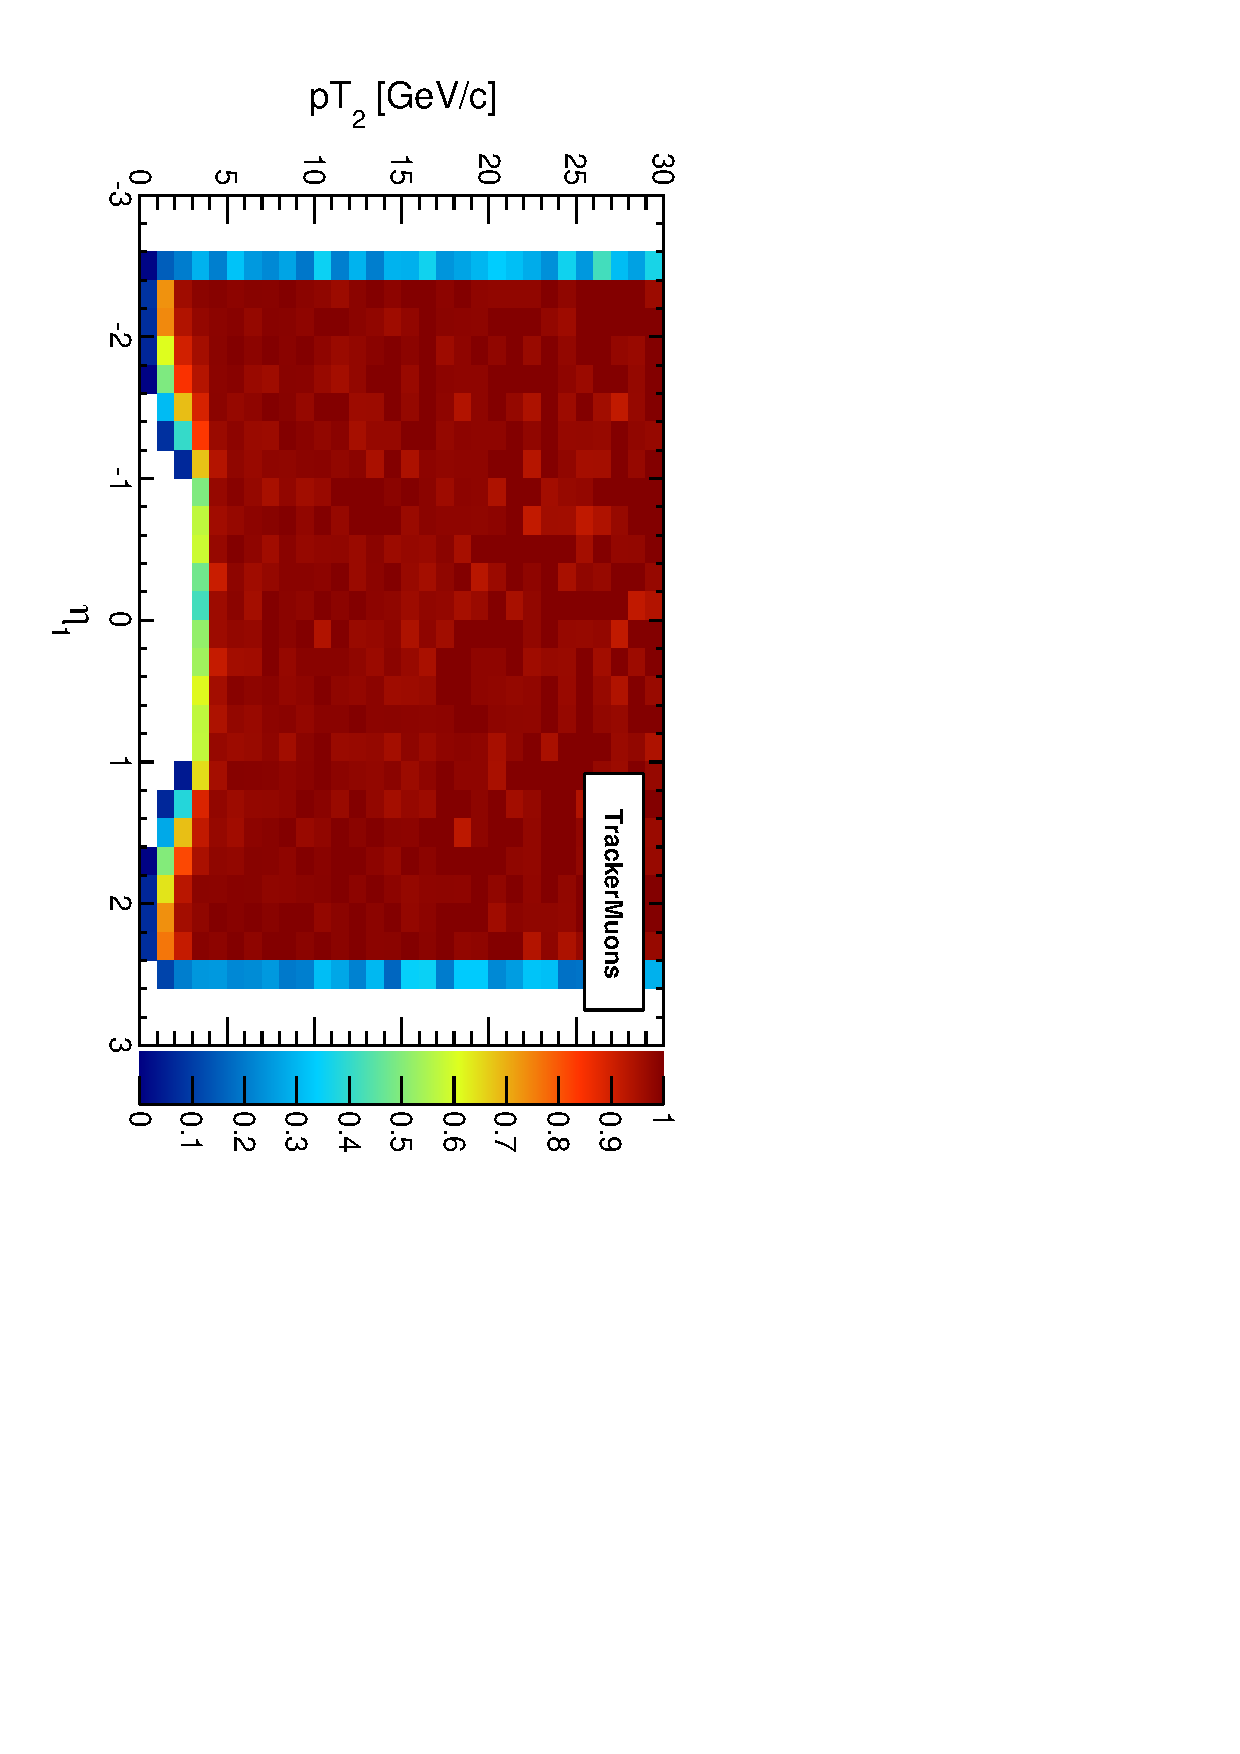
\includegraphics[height=0.5\linewidth, angle=90]{fig/acceptance_plot/pt2vseta1_TrackerMuons.pdf}
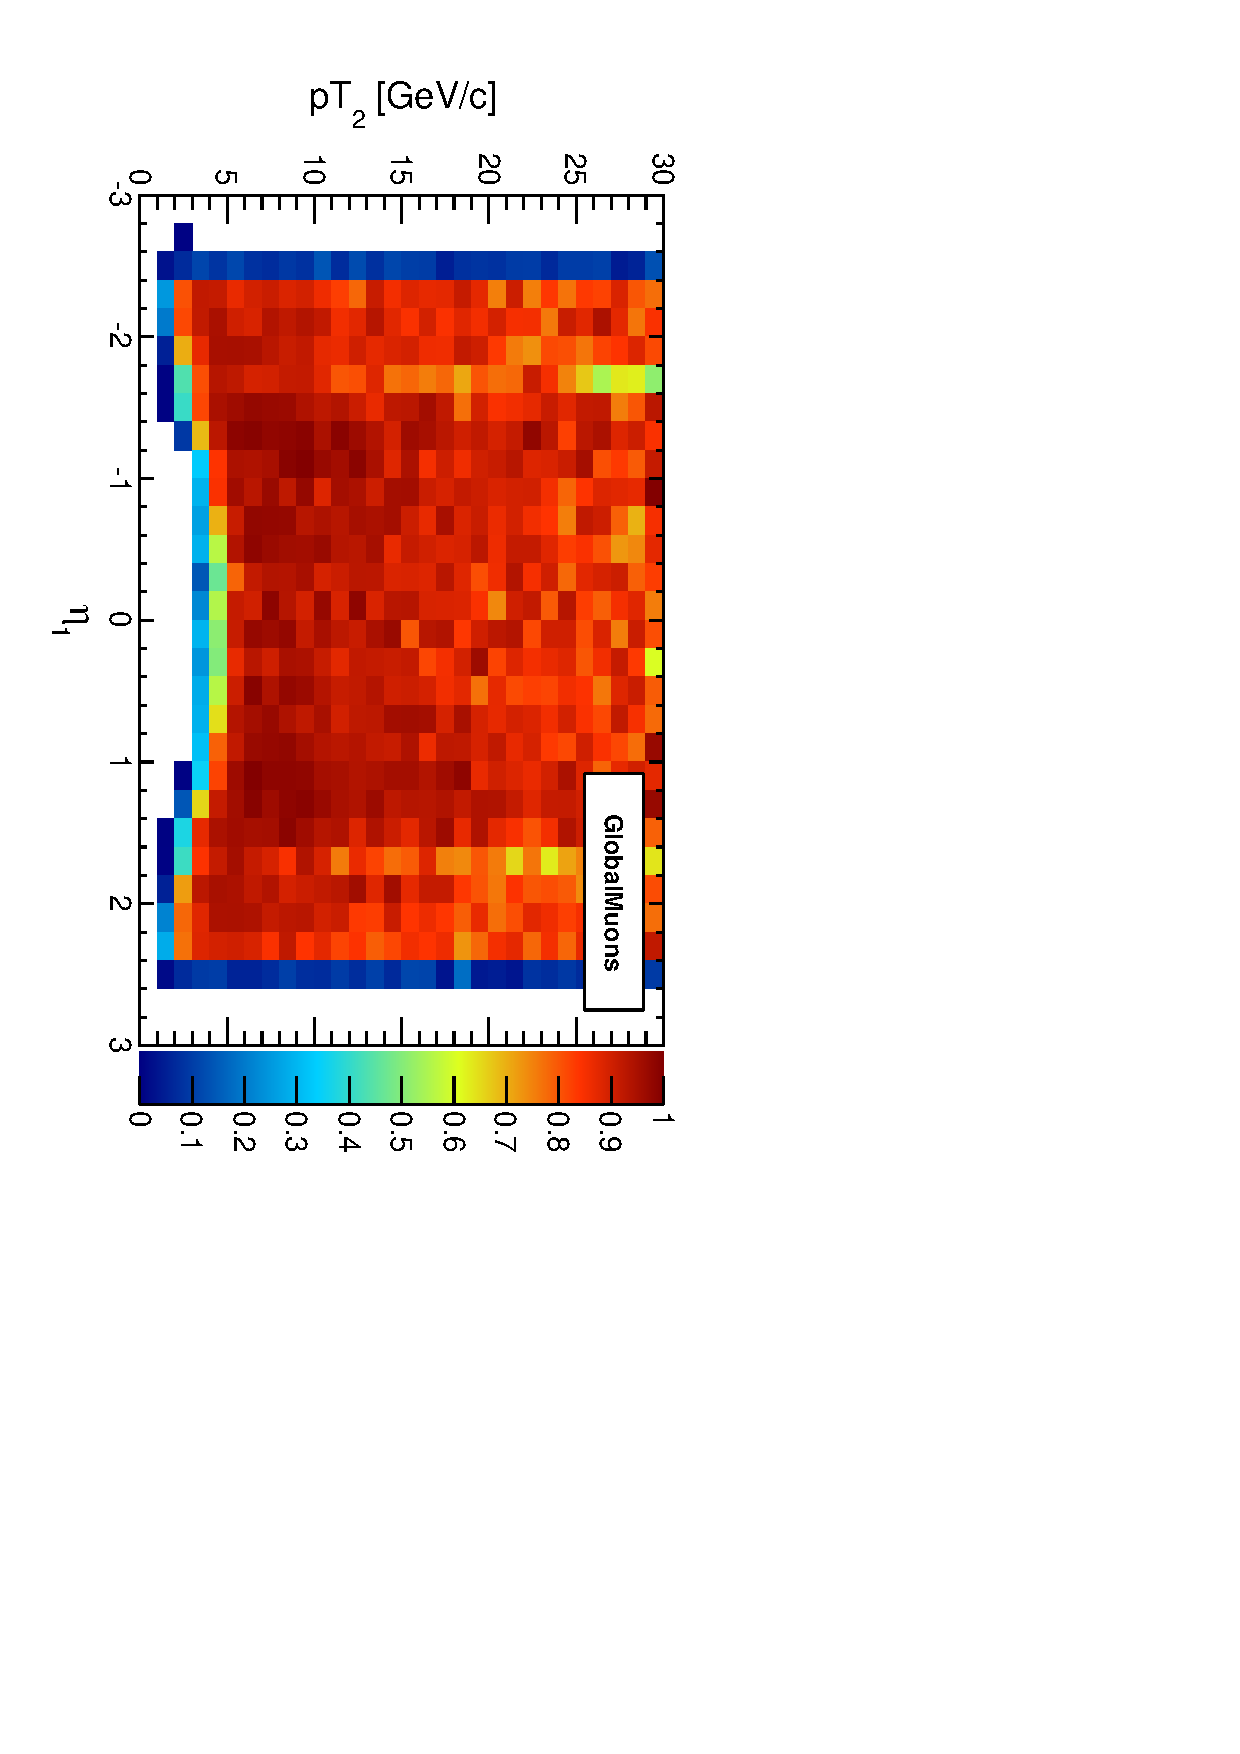
\includegraphics[height=0.5\linewidth, angle=90]{fig/acceptance_plot/pt2vseta1_GlobalMuons.pdf}

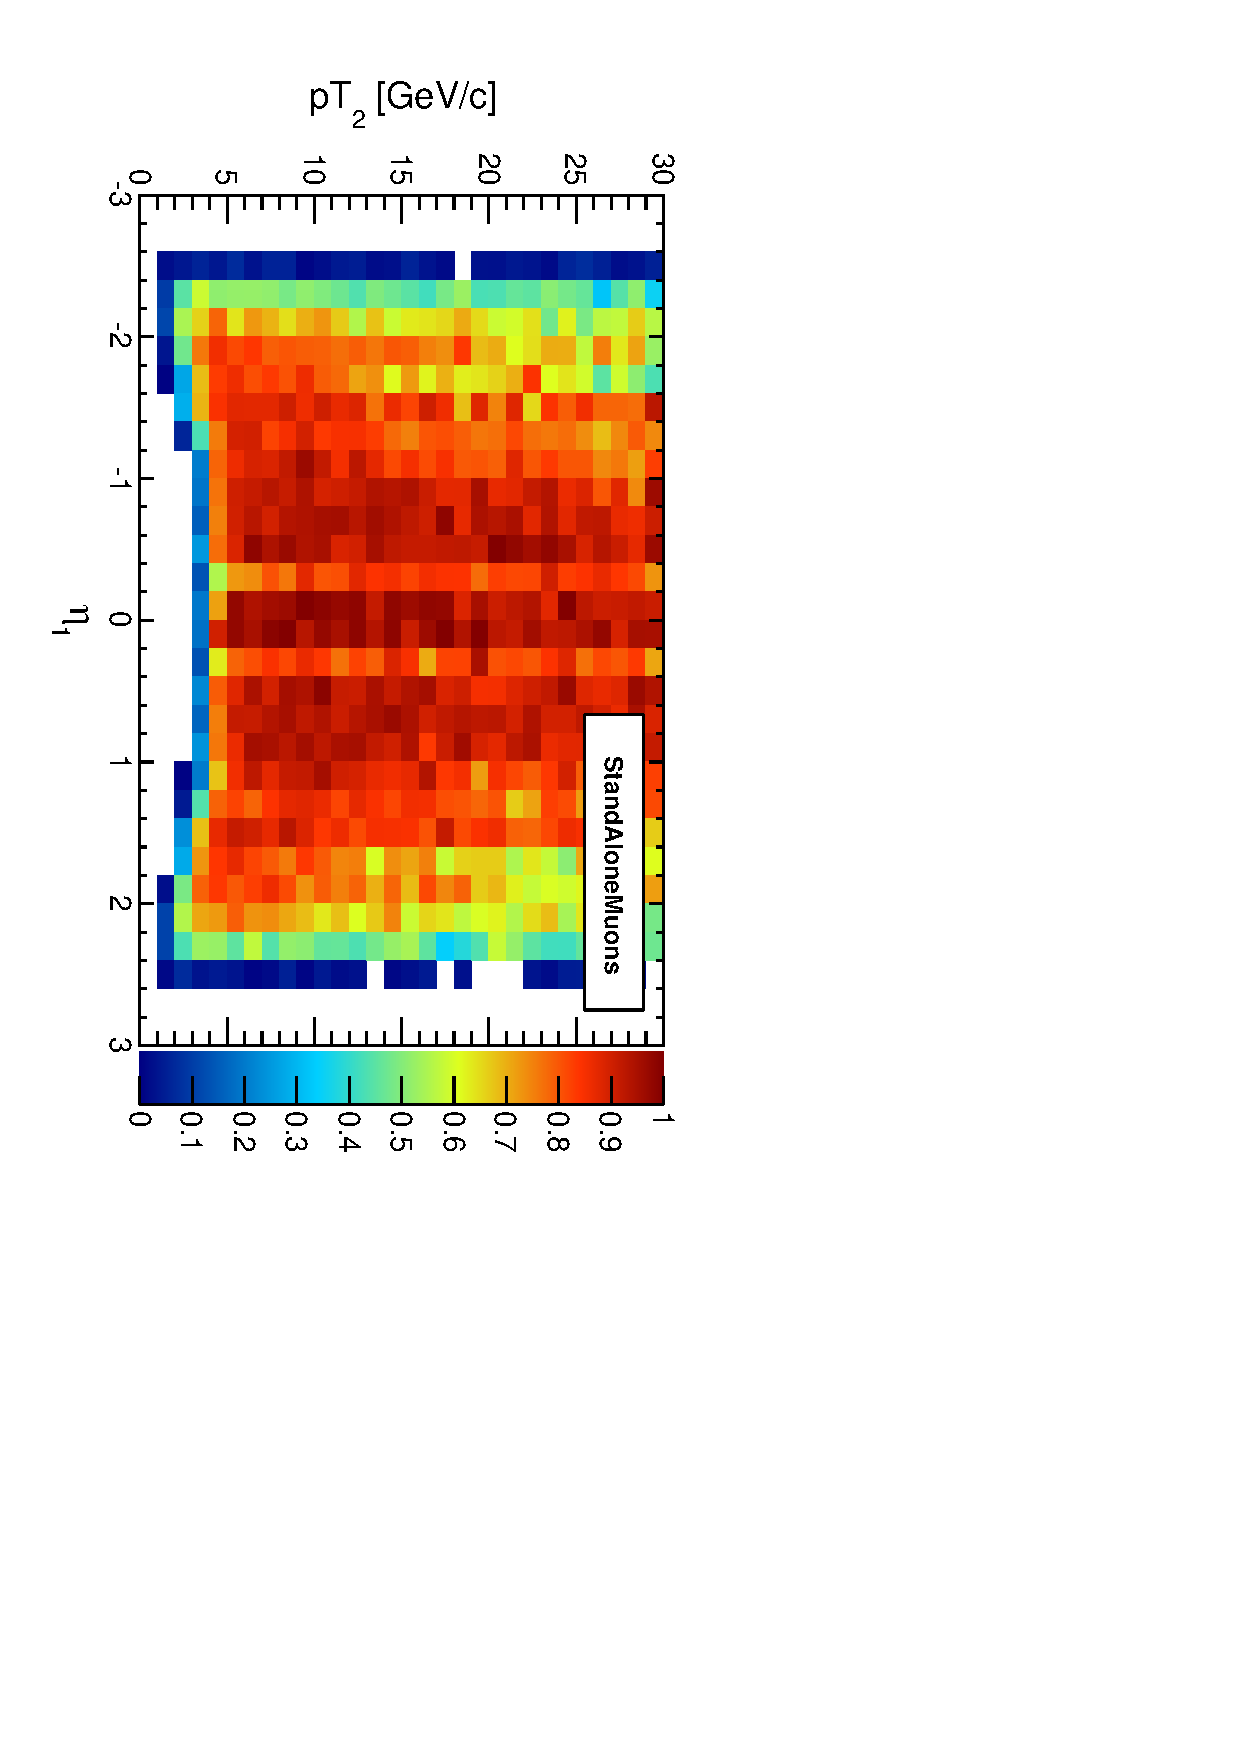
\includegraphics[height=0.5\linewidth, angle=90]{fig/acceptance_plot/pt2vseta1_StandAloneUpdatedDefault.pdf}
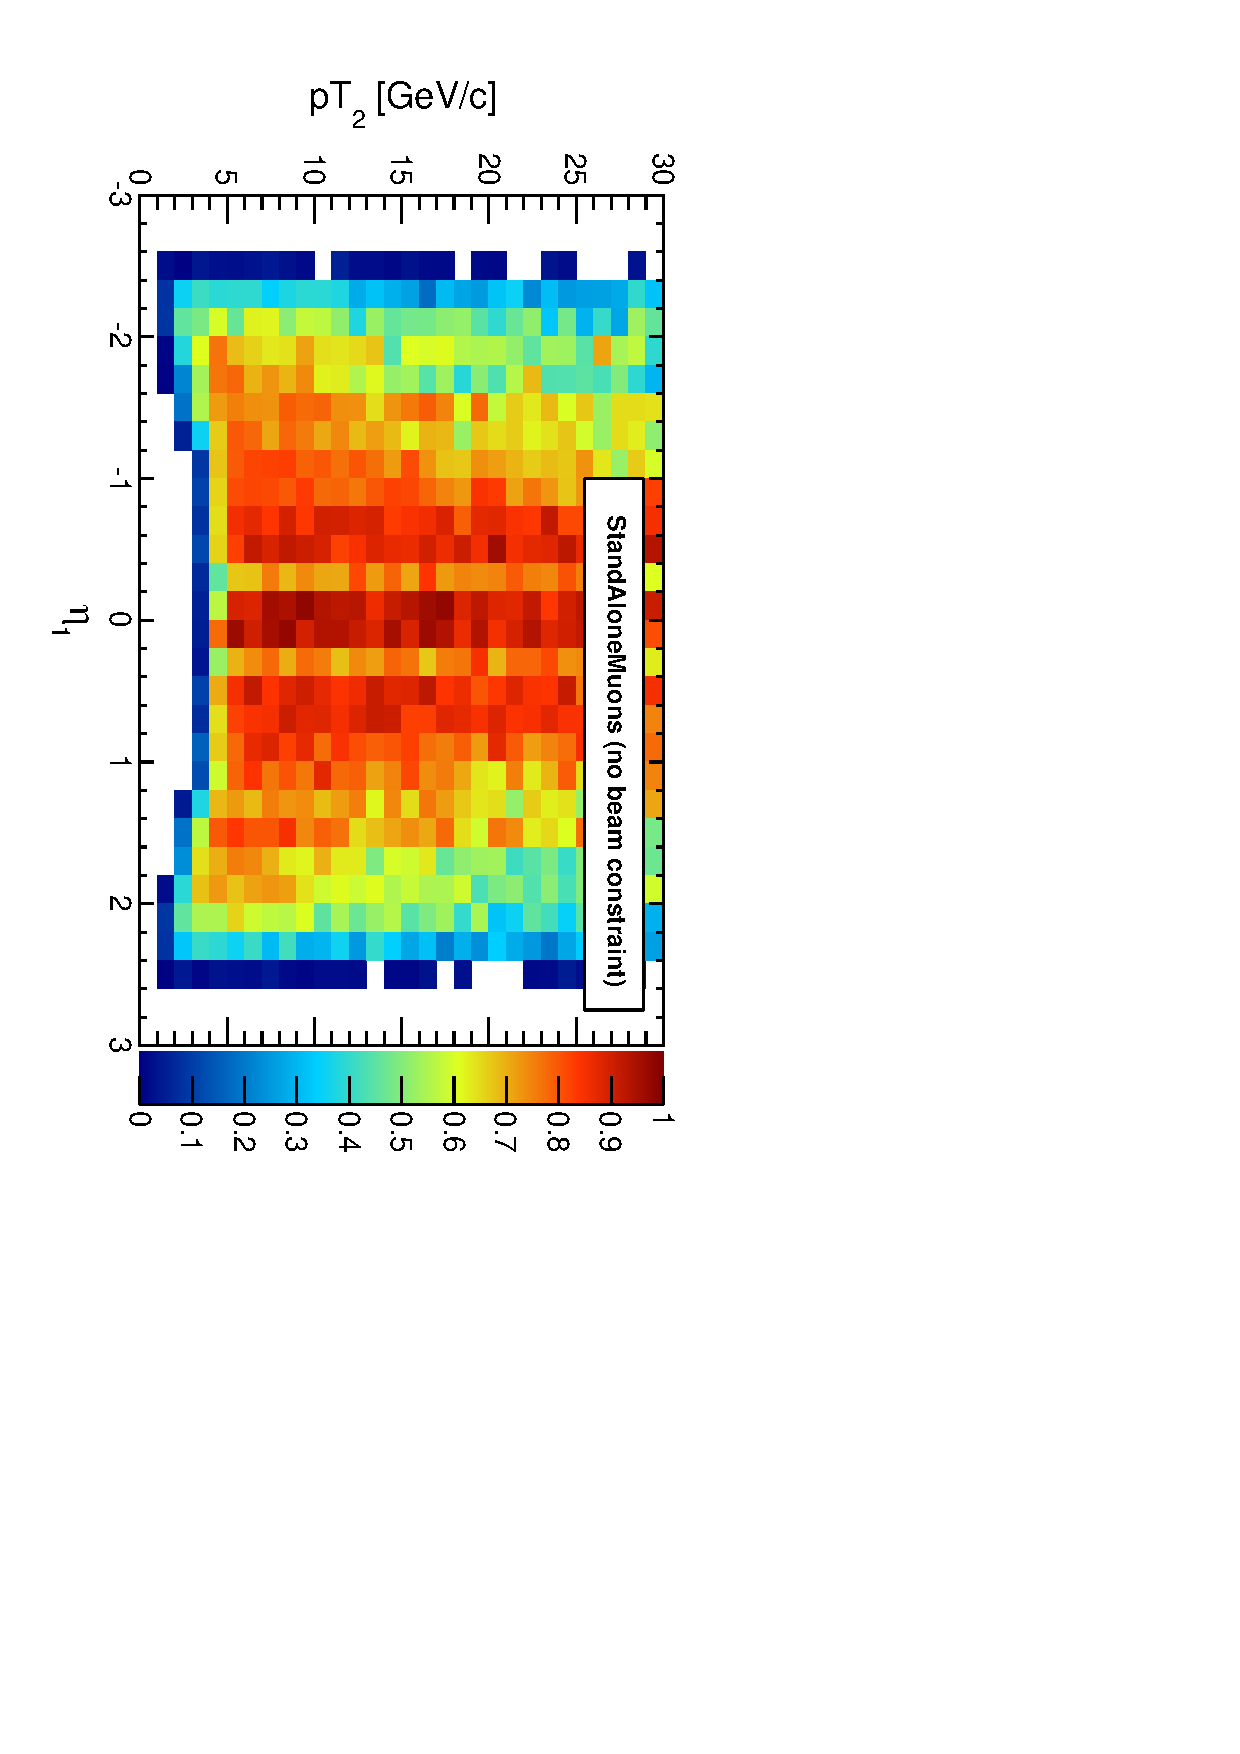
\includegraphics[height=0.5\linewidth, angle=90]{fig/acceptance_plot/pt2vseta1_StandAloneDefault.pdf}

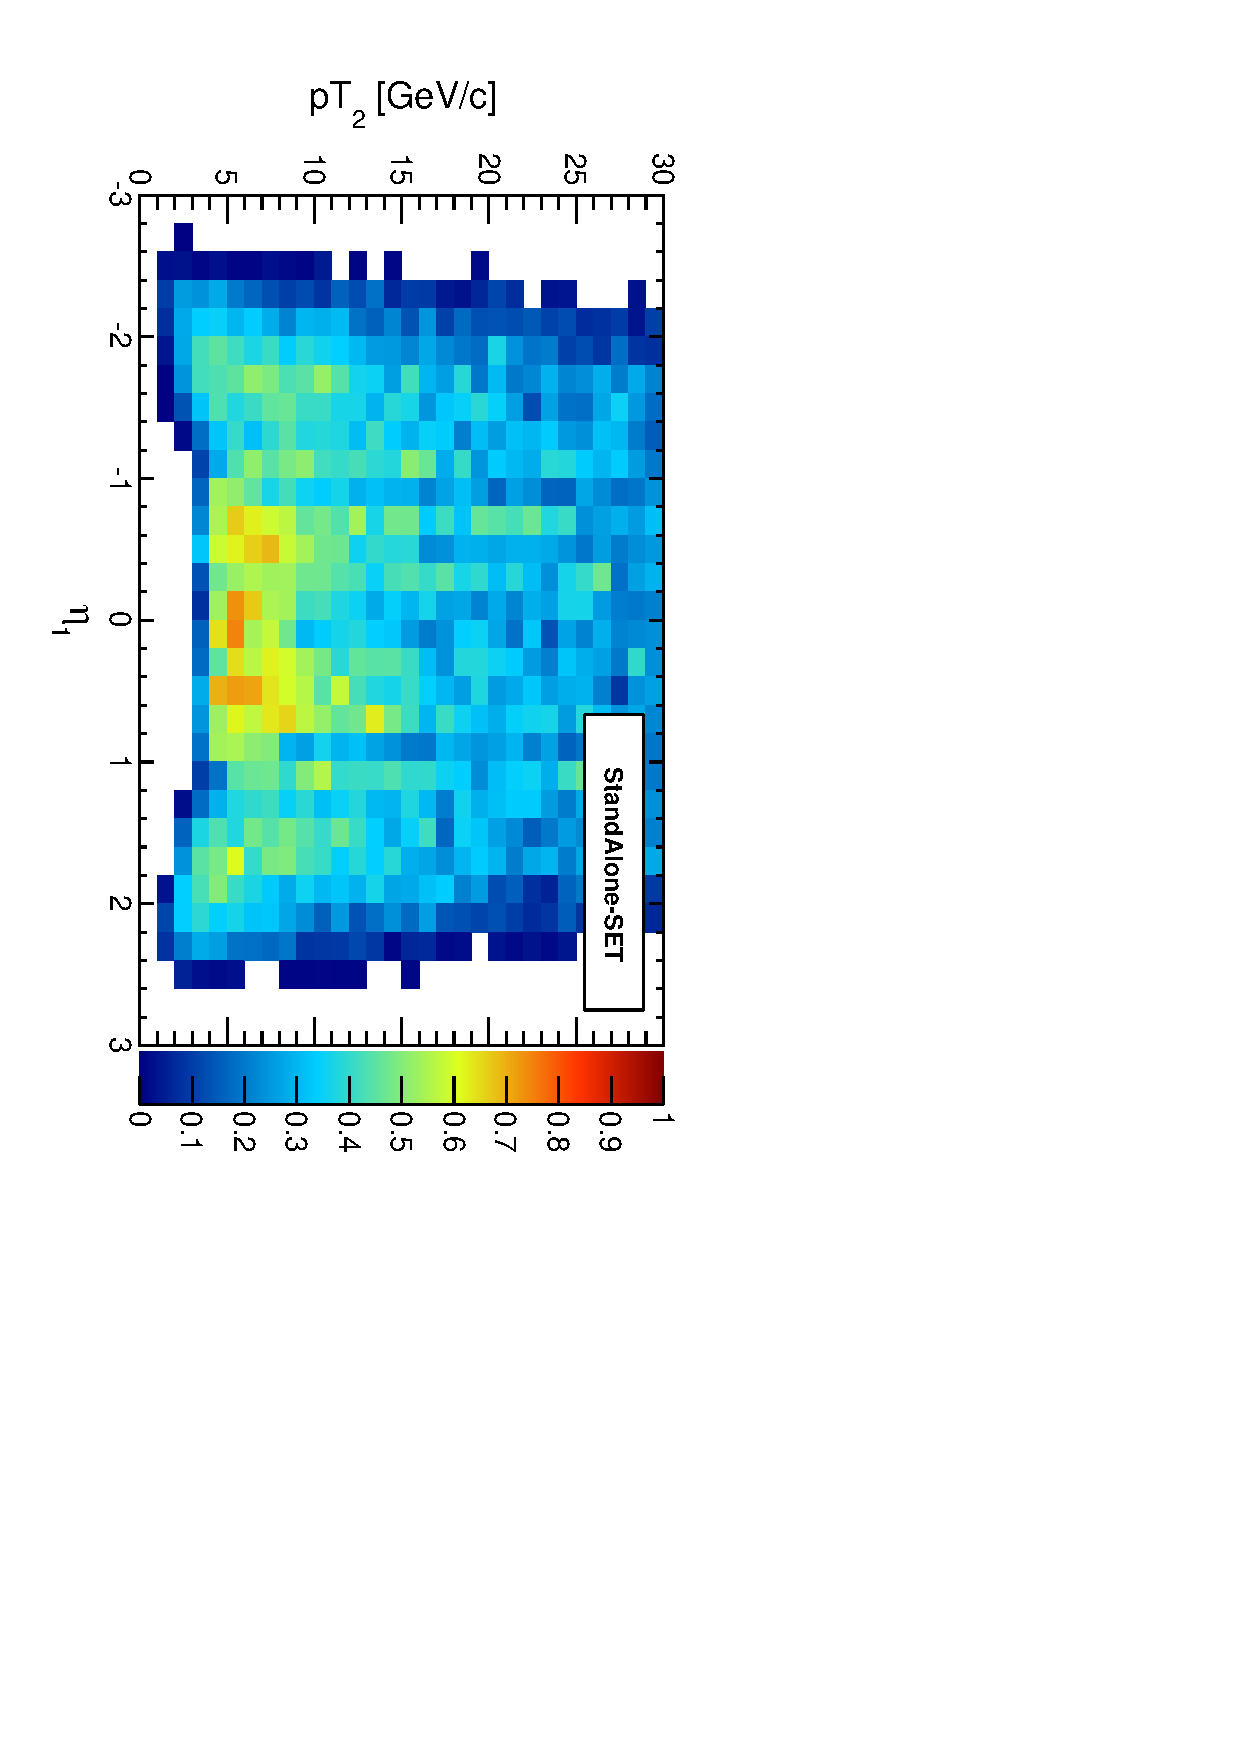
\includegraphics[height=0.5\linewidth, angle=90]{fig/acceptance_plot/pt2vseta1_StandAloneUpdatedSET.pdf}
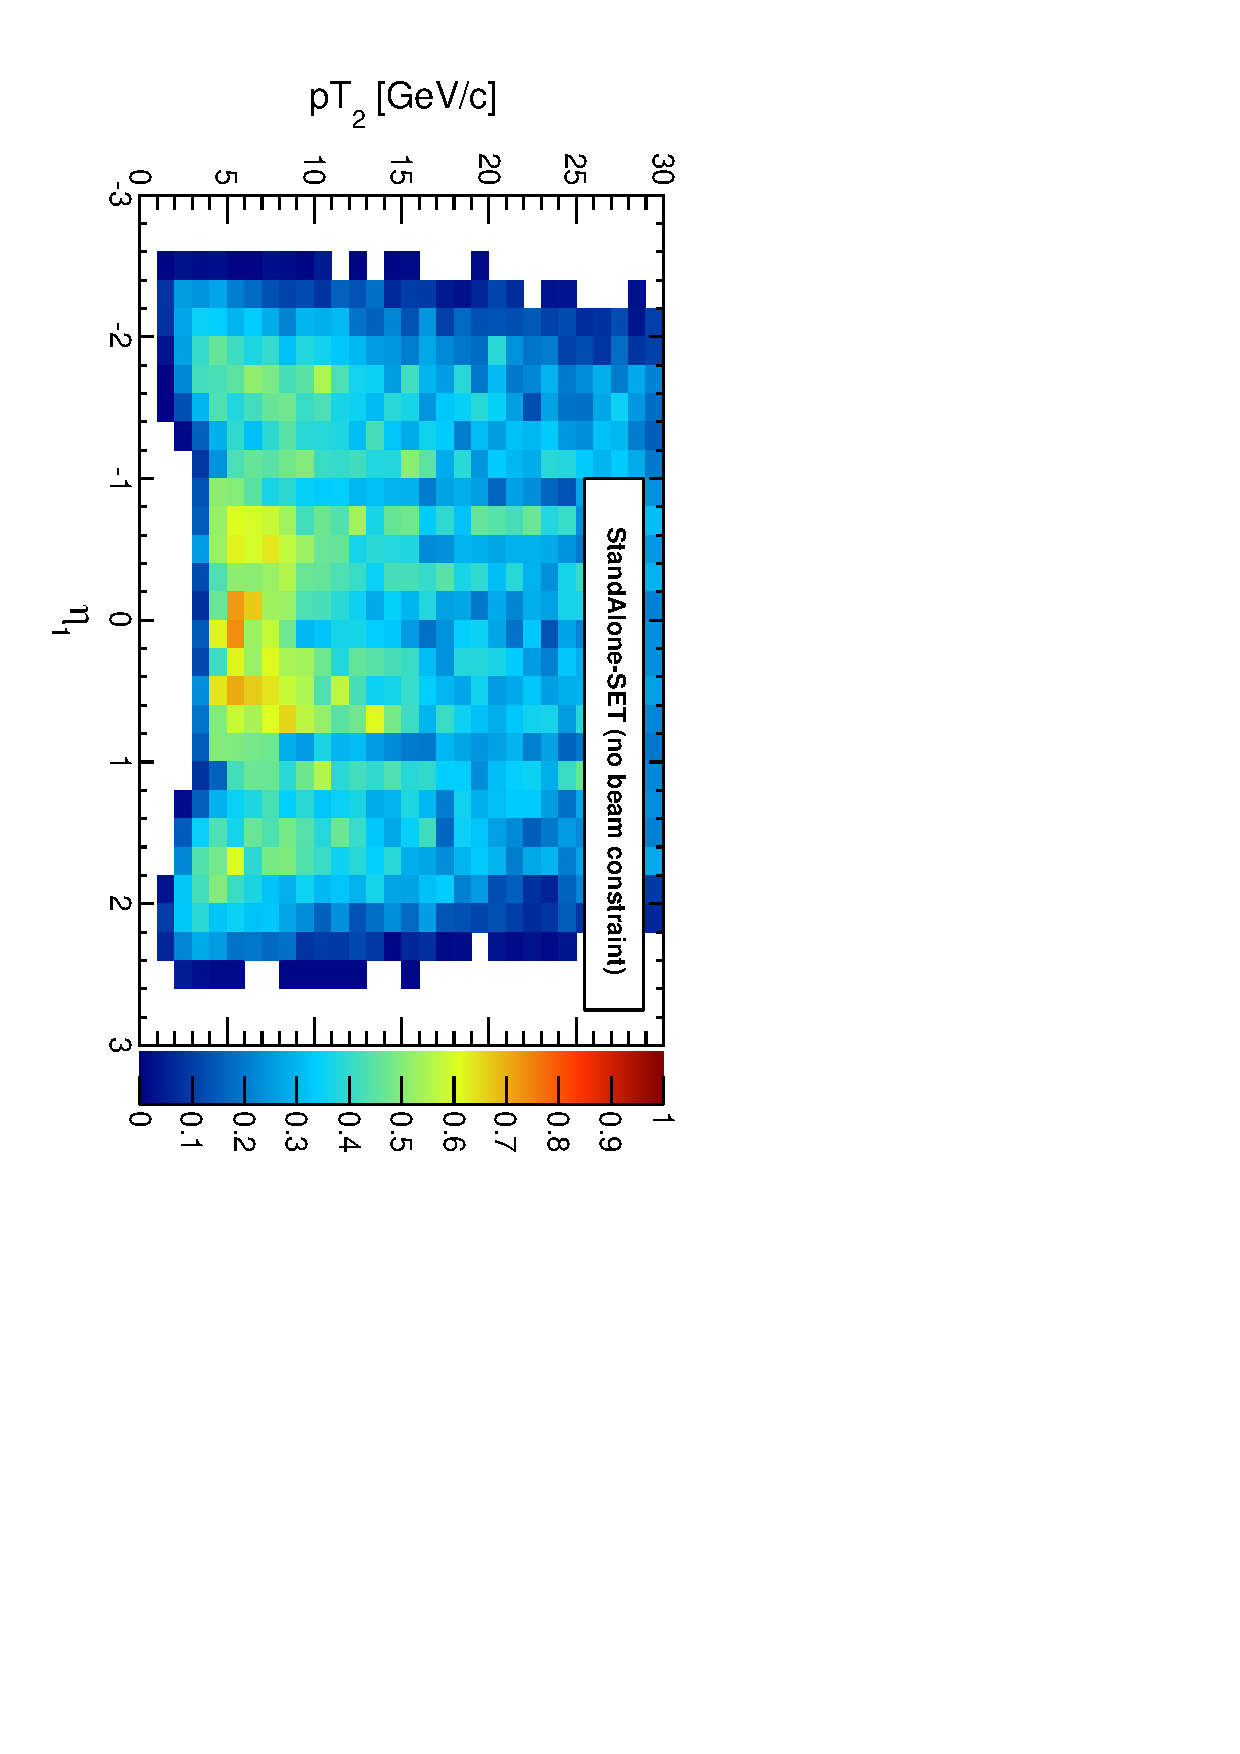
\includegraphics[height=0.5\linewidth, angle=90]{fig/acceptance_plot/pt2vseta1_StandAloneSET.pdf}

\caption{Acceptance region and efficiency for different reconstruction
  methods.  $pT_2$ is the second-highest $p_T$ muon in the event,
  $\eta_1$ is the largest-magnitude pseudorapidity in the event.
  Denominator: all generated events; numerator: reconstructed
  and MC-matched $\mu^+$ and $\mu^-$. \label{fig:pt2vseta1}}
\end{figure}

\begin{figure}[p]
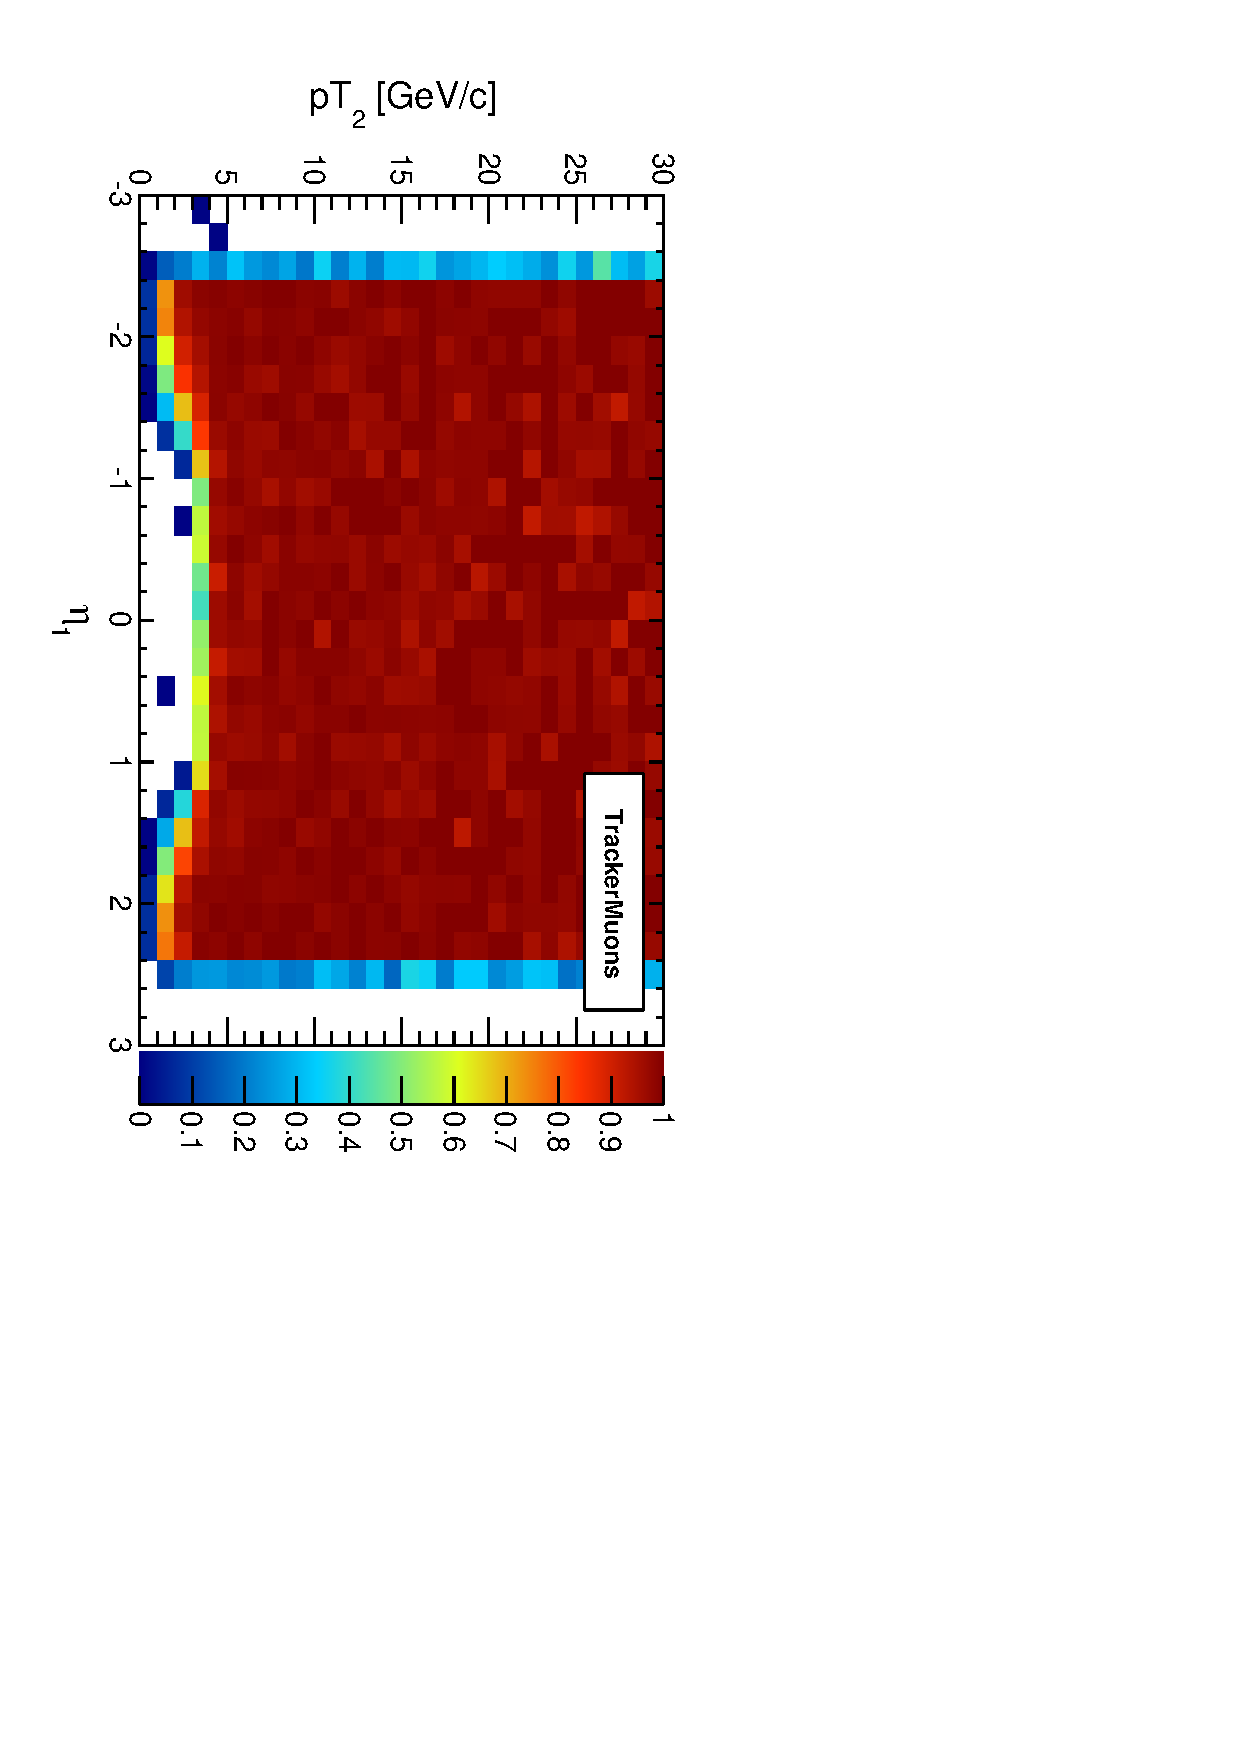
\includegraphics[height=0.5\linewidth, angle=90]{fig/acceptanceNoMCMatch_plot/pt2vseta1_TrackerMuons.pdf}
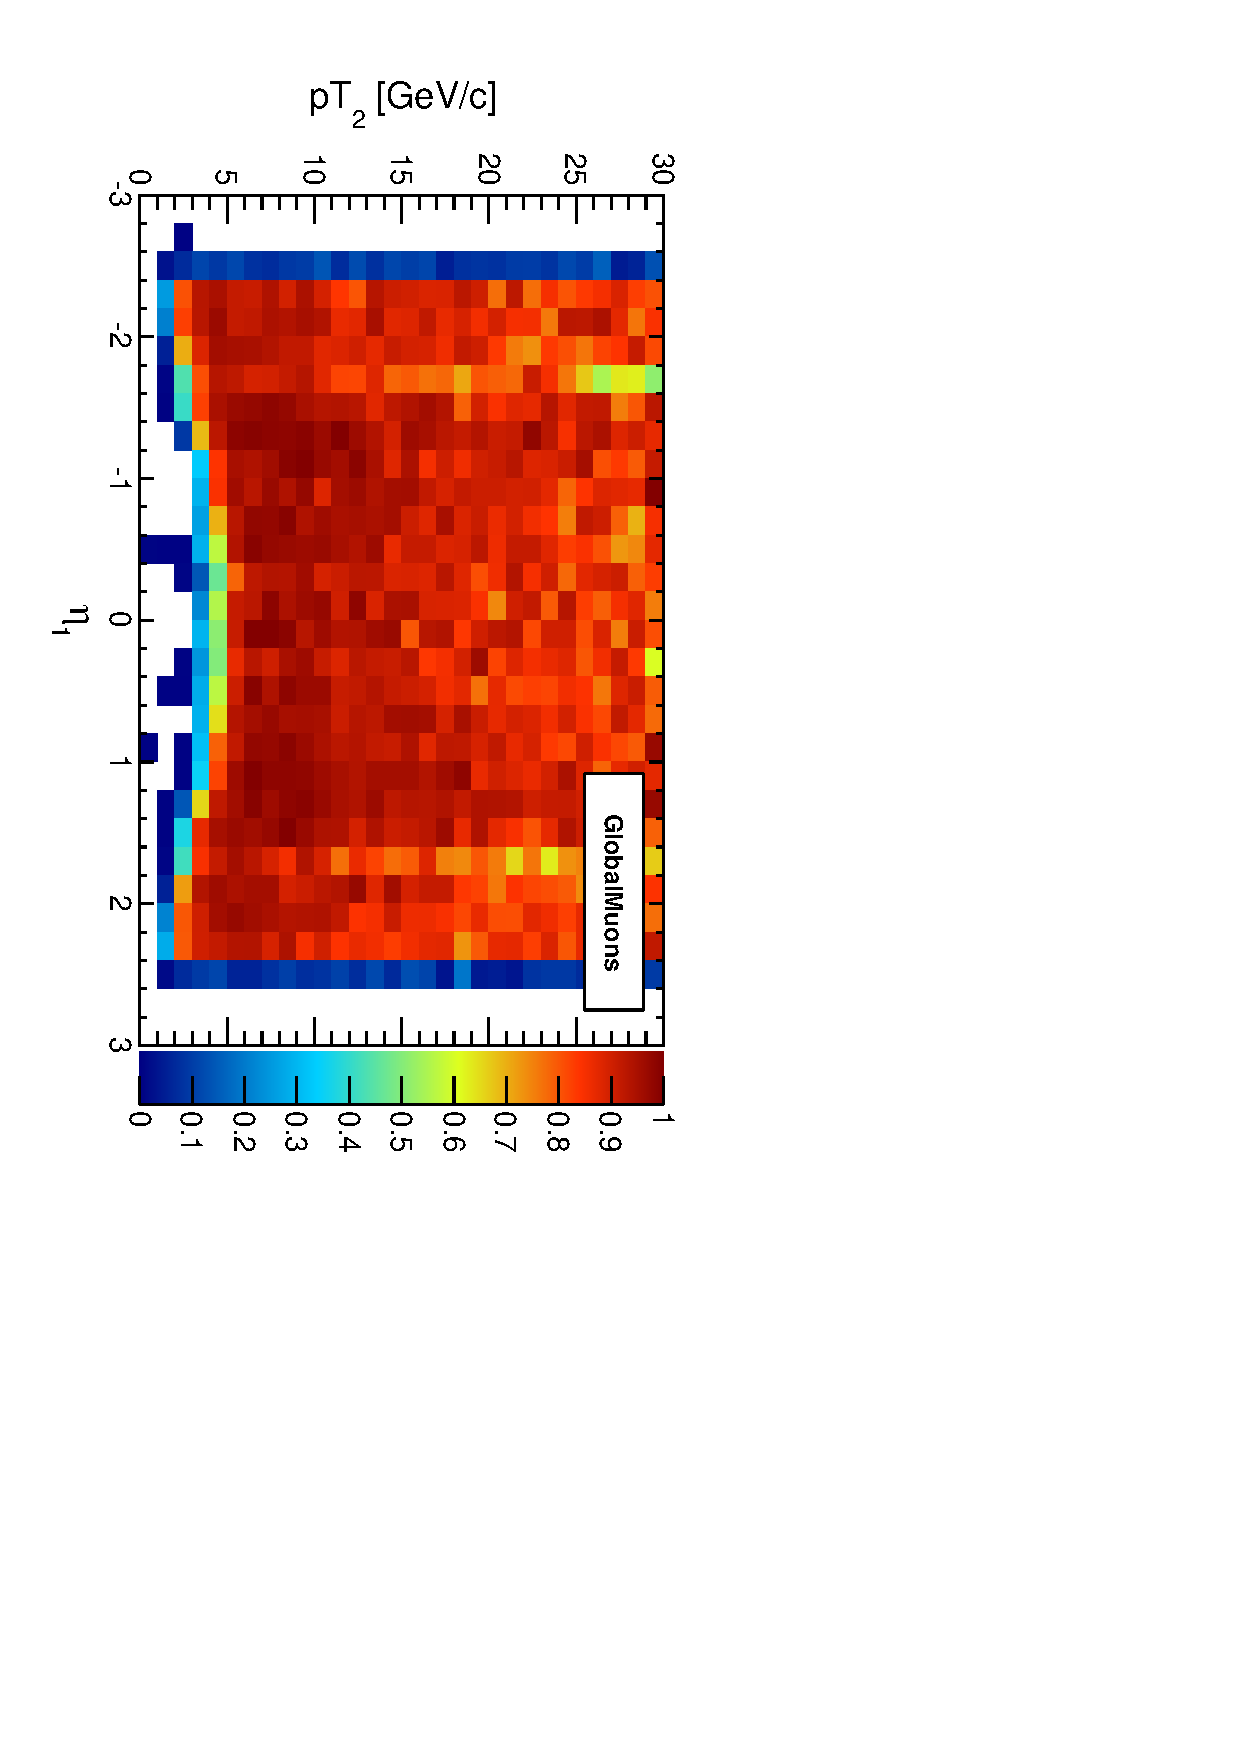
\includegraphics[height=0.5\linewidth, angle=90]{fig/acceptanceNoMCMatch_plot/pt2vseta1_GlobalMuons.pdf}

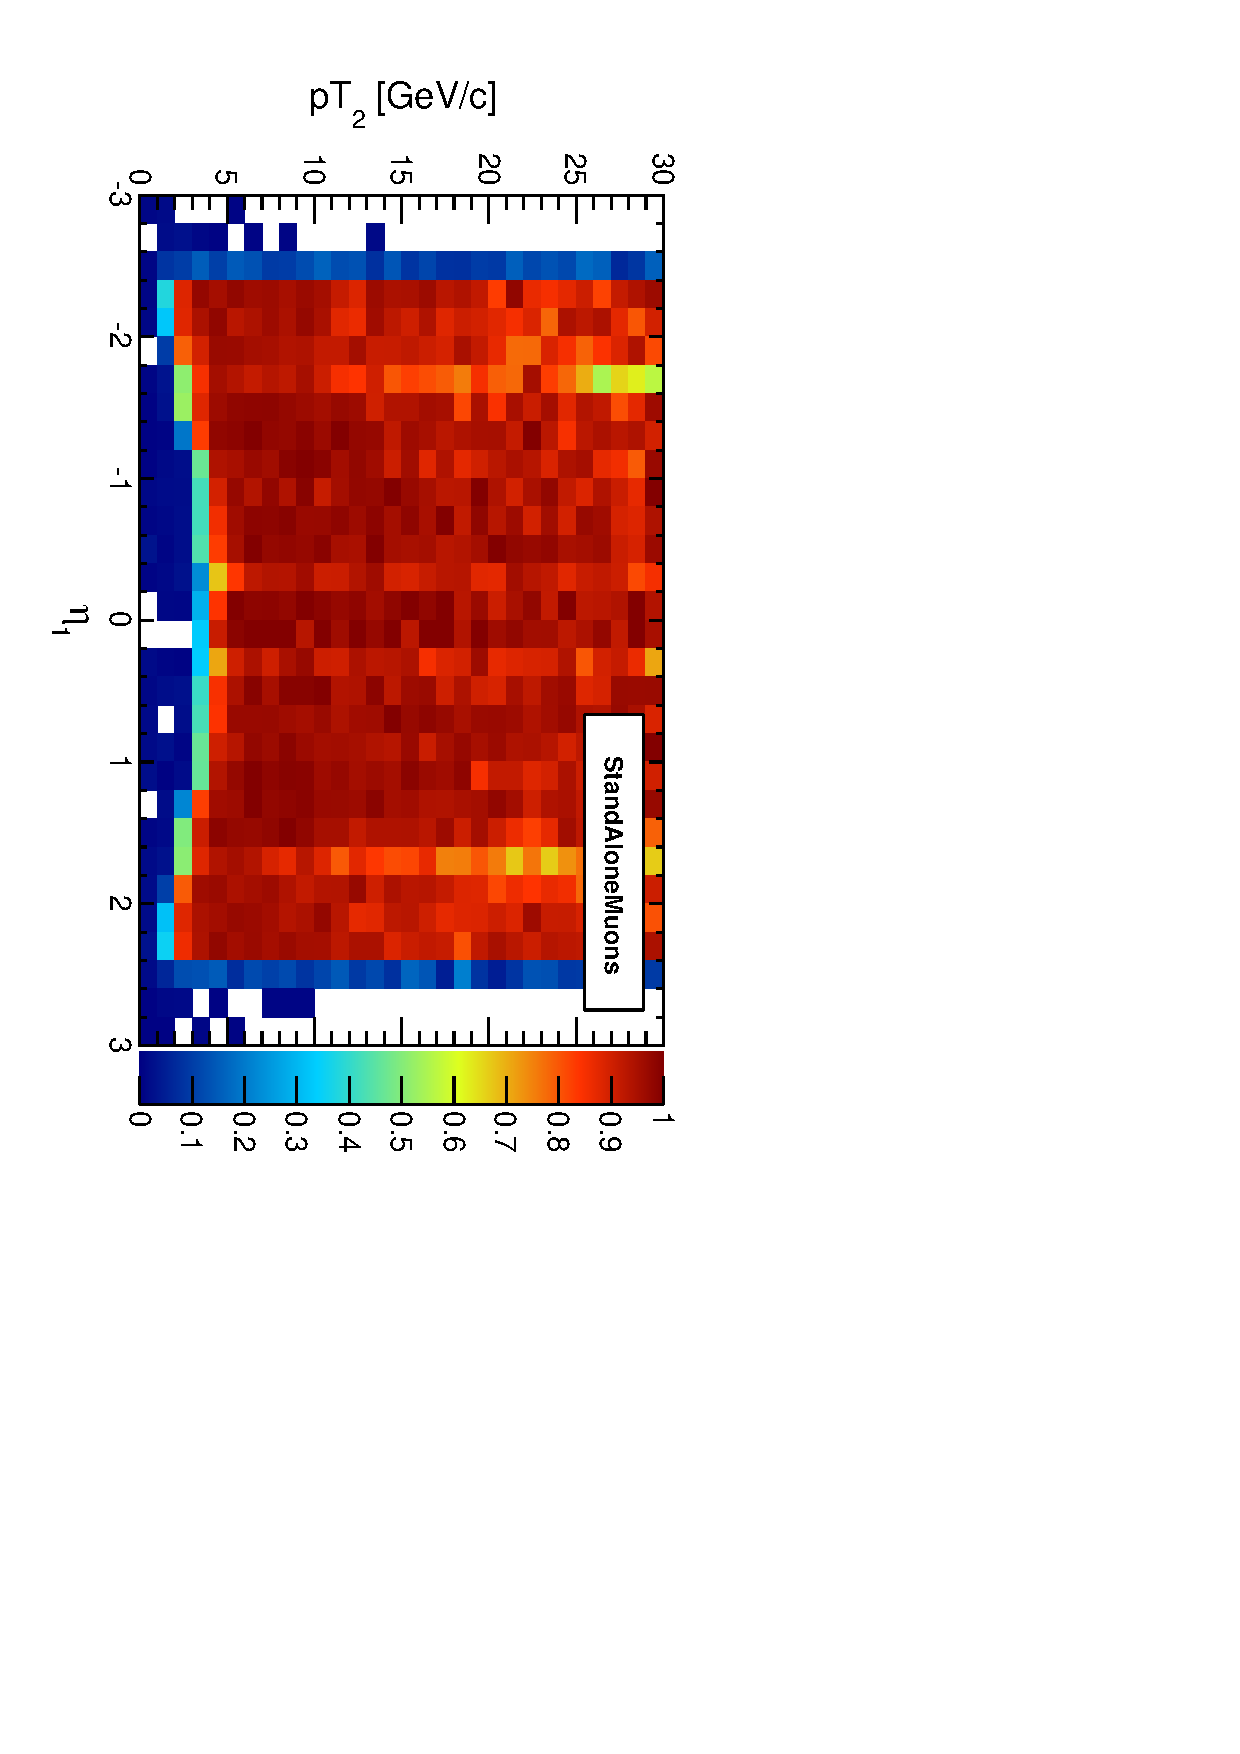
\includegraphics[height=0.5\linewidth, angle=90]{fig/acceptanceNoMCMatch_plot/pt2vseta1_StandAloneUpdatedDefault.pdf}
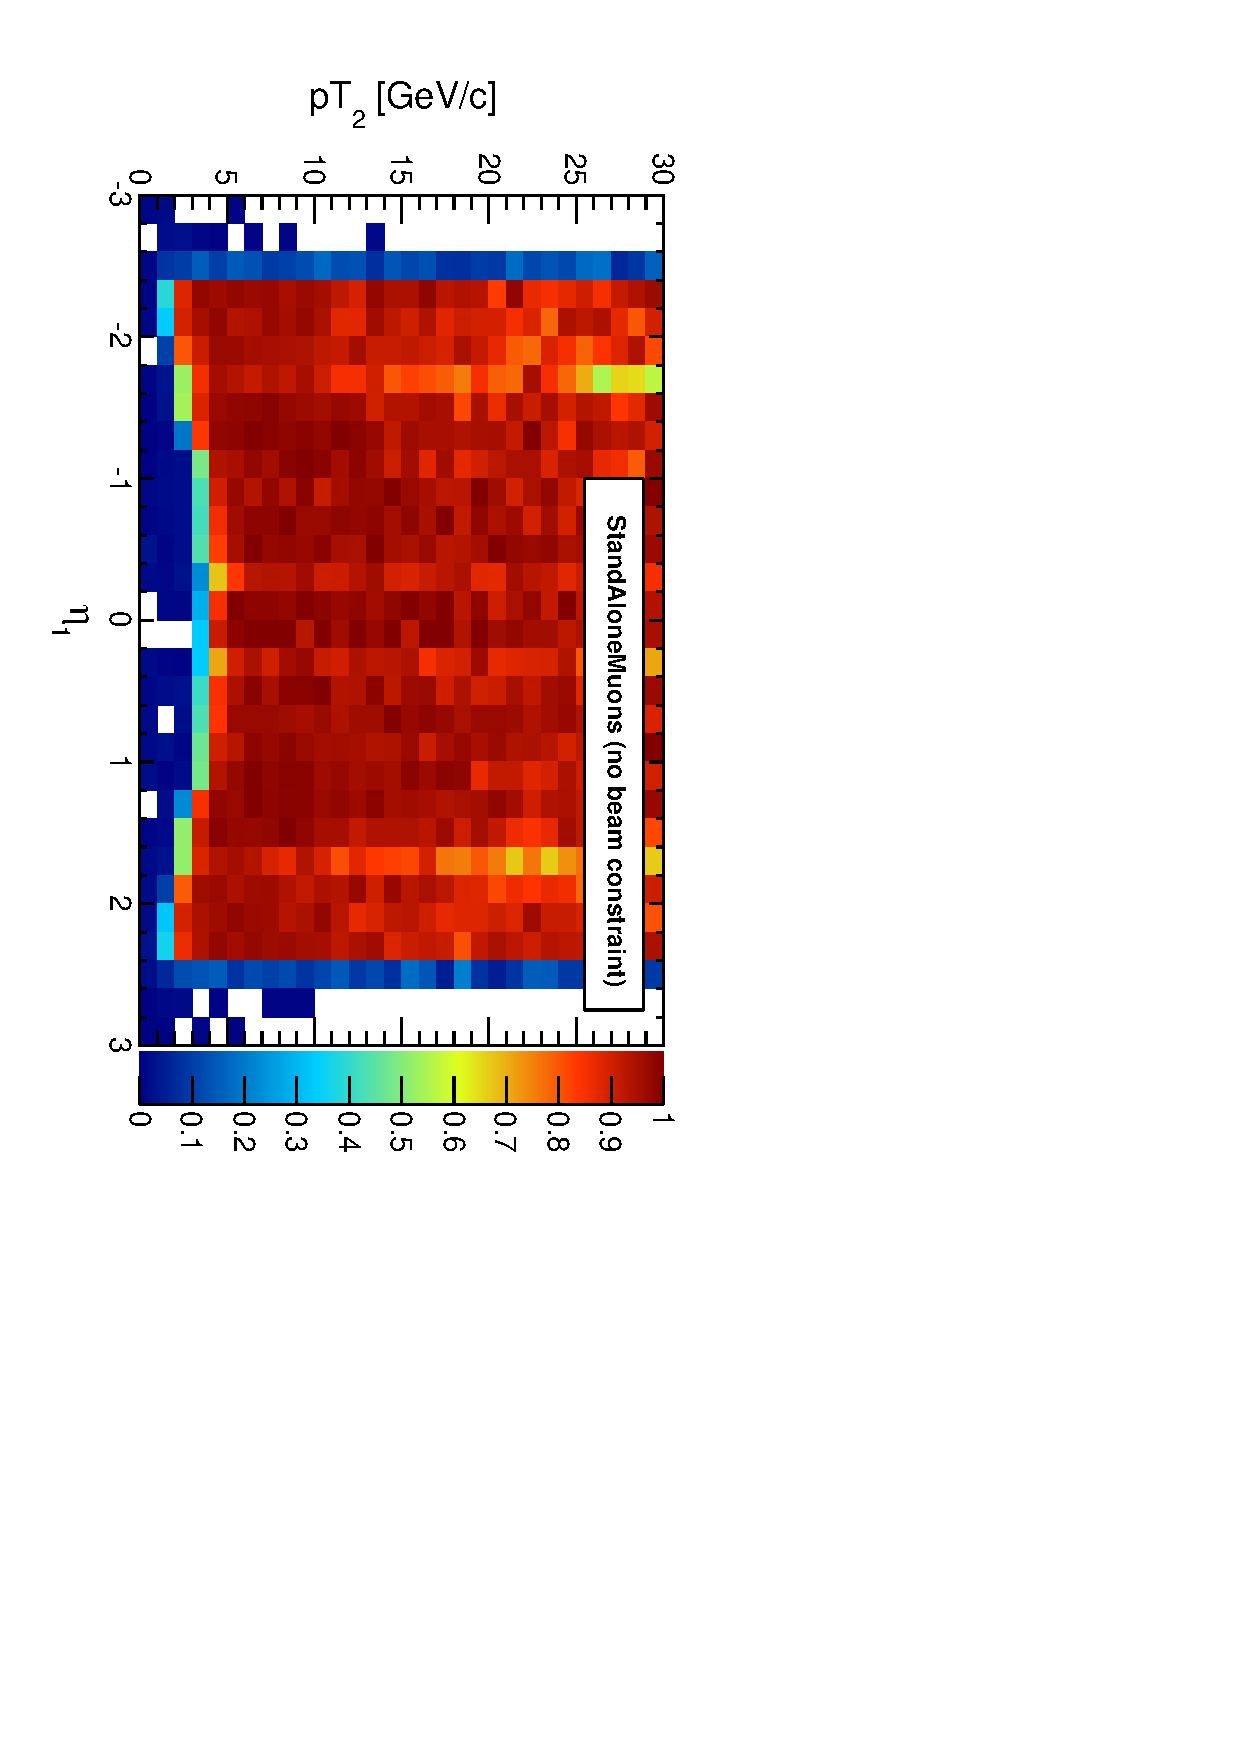
\includegraphics[height=0.5\linewidth, angle=90]{fig/acceptanceNoMCMatch_plot/pt2vseta1_StandAloneDefault.pdf}

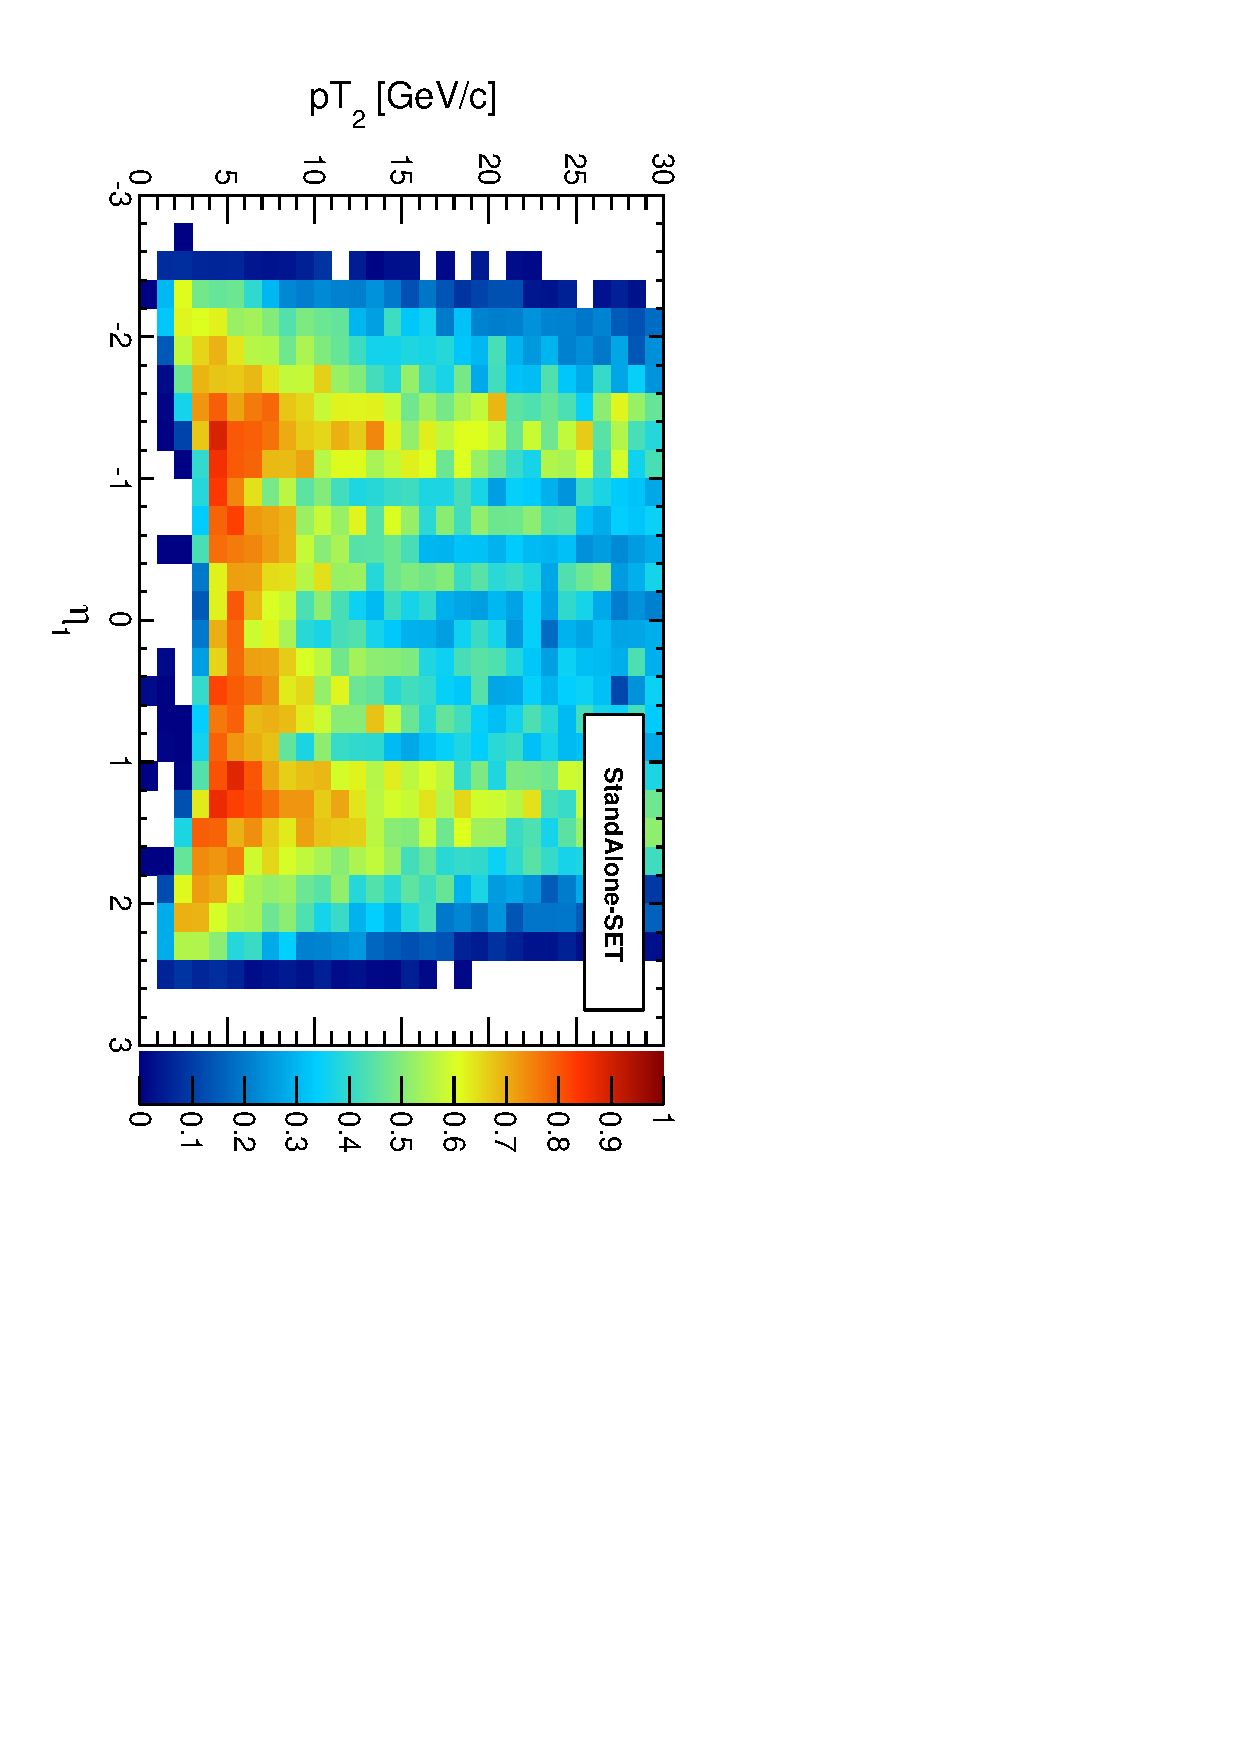
\includegraphics[height=0.5\linewidth, angle=90]{fig/acceptanceNoMCMatch_plot/pt2vseta1_StandAloneUpdatedSET.pdf}
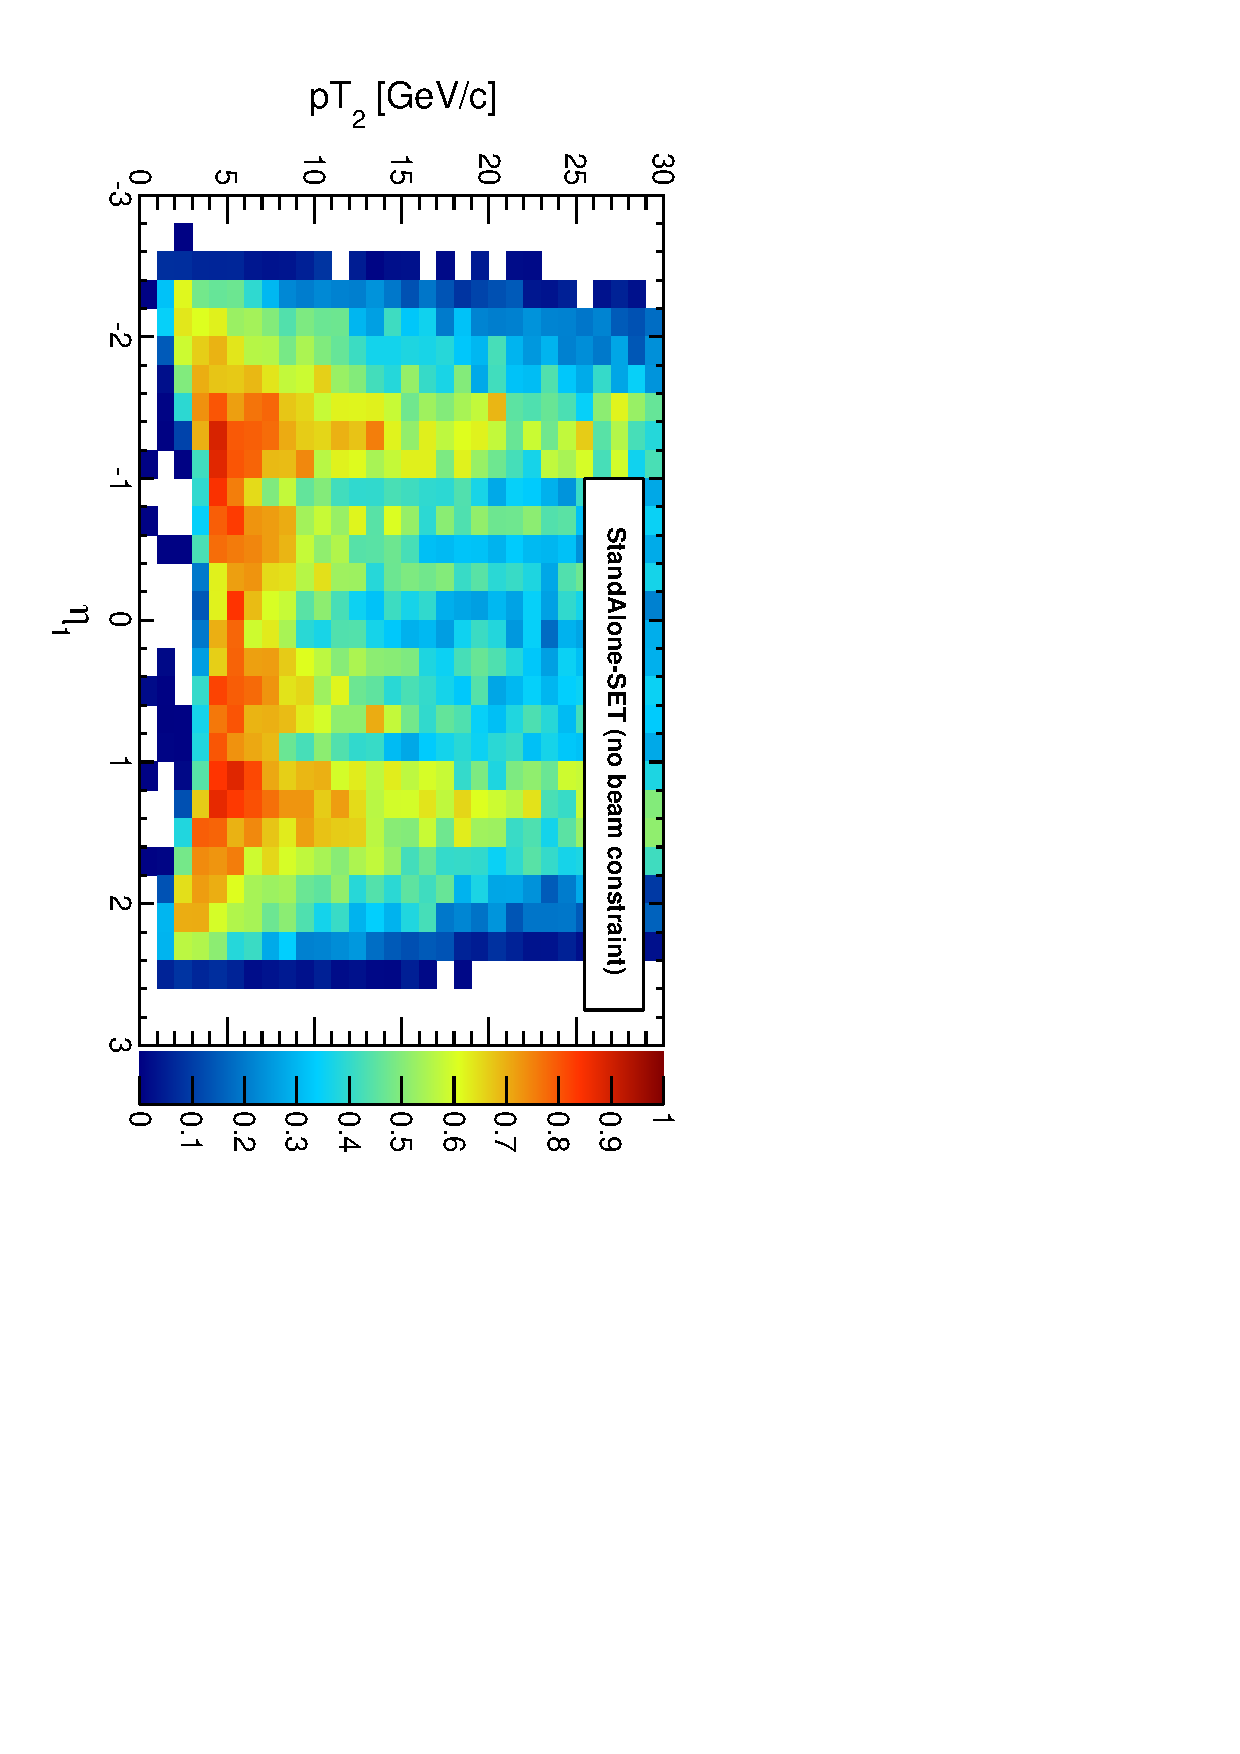
\includegraphics[height=0.5\linewidth, angle=90]{fig/acceptanceNoMCMatch_plot/pt2vseta1_StandAloneSET.pdf}

\caption{Same as Fig.~\ref{fig:pt2vseta1}, except that numerator only requires two reconstructed muons (no MC-matching).  \label{fig:pt2vseta1NoMCMatch}}
\end{figure}

\begin{figure}
\begin{center}
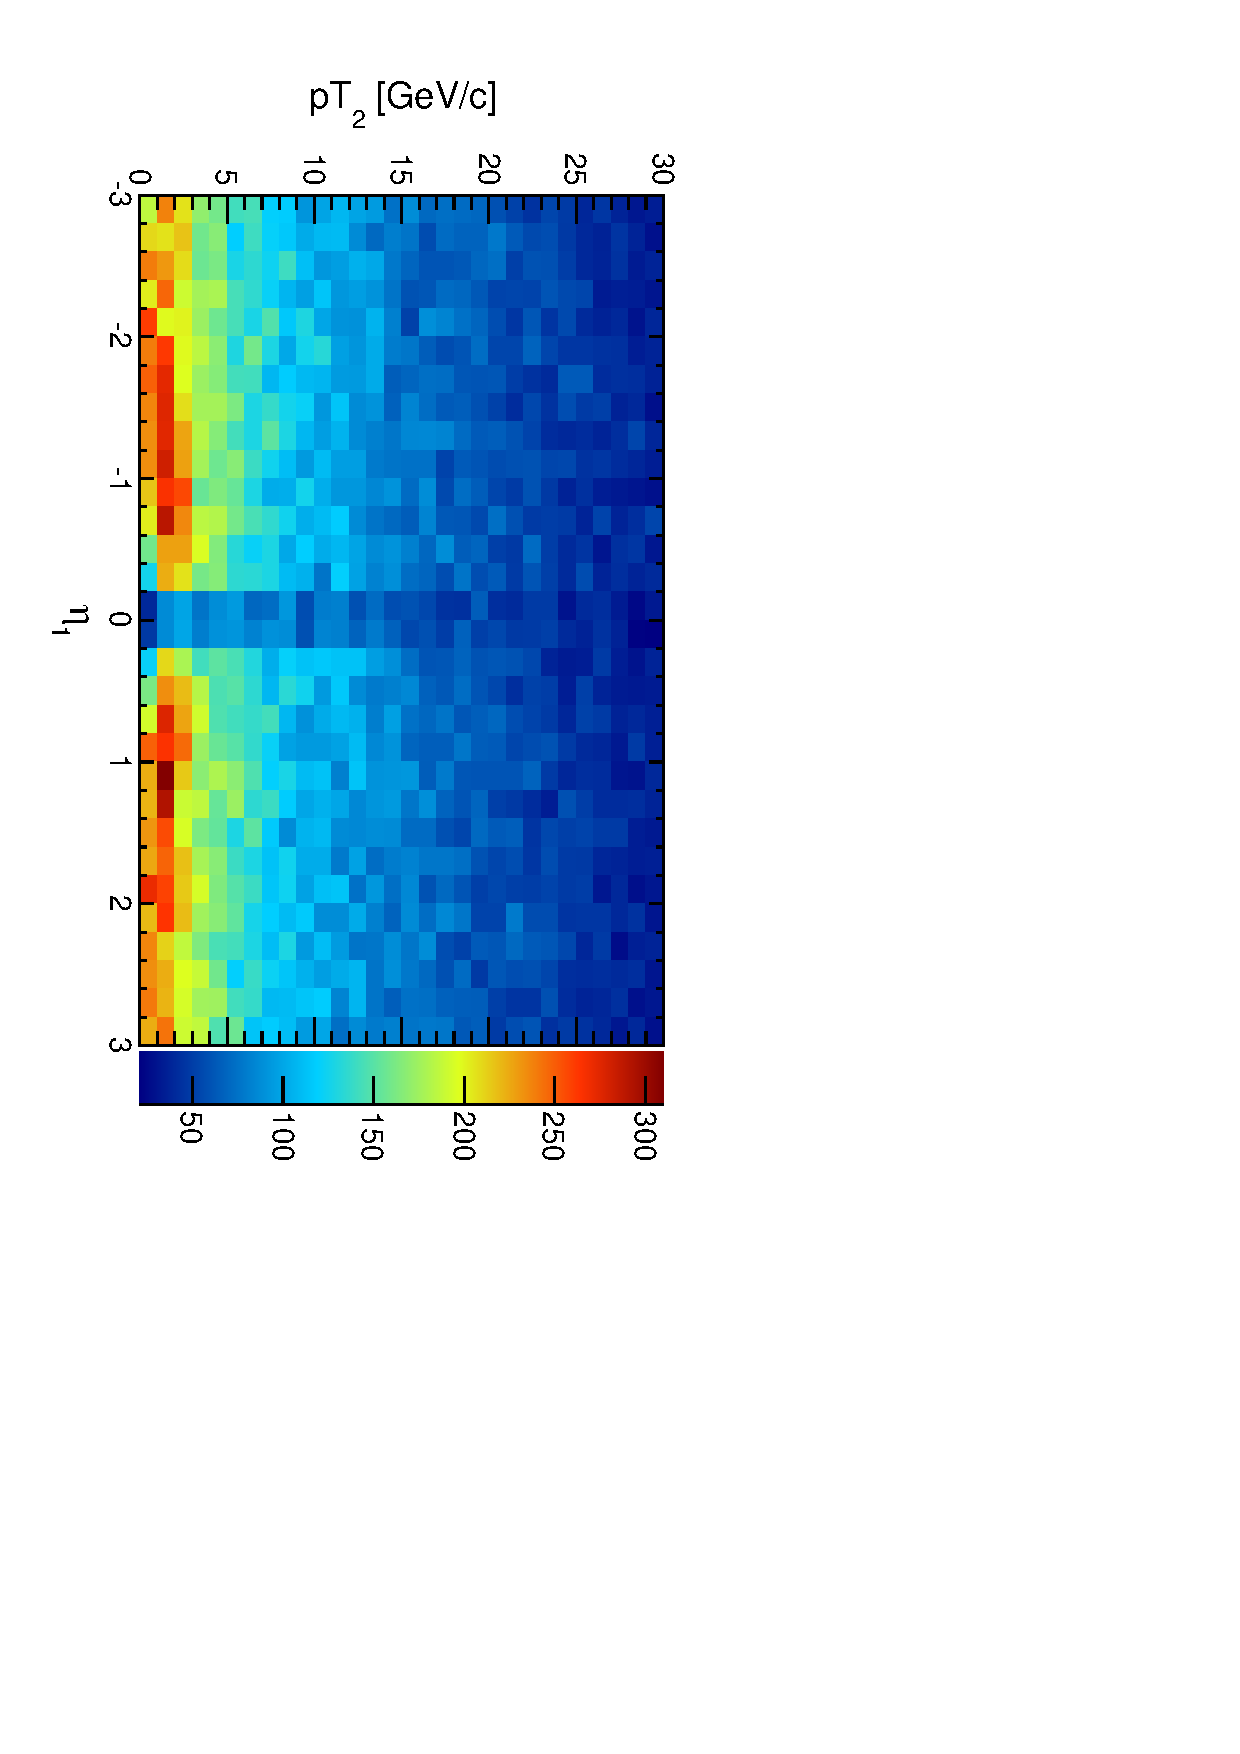
\includegraphics[height=0.5\linewidth, angle=90]{fig/acceptance_plot/pt2vseta1_TrackerMuons_denominator.pdf}
\end{center}
\caption{Denominator of Figs.~\ref{fig:pt2vseta1} and \ref{fig:pt2vseta1NoMCMatch}. \label{fig:pt2vseta1Denominator}}
\end{figure}

\begin{figure}
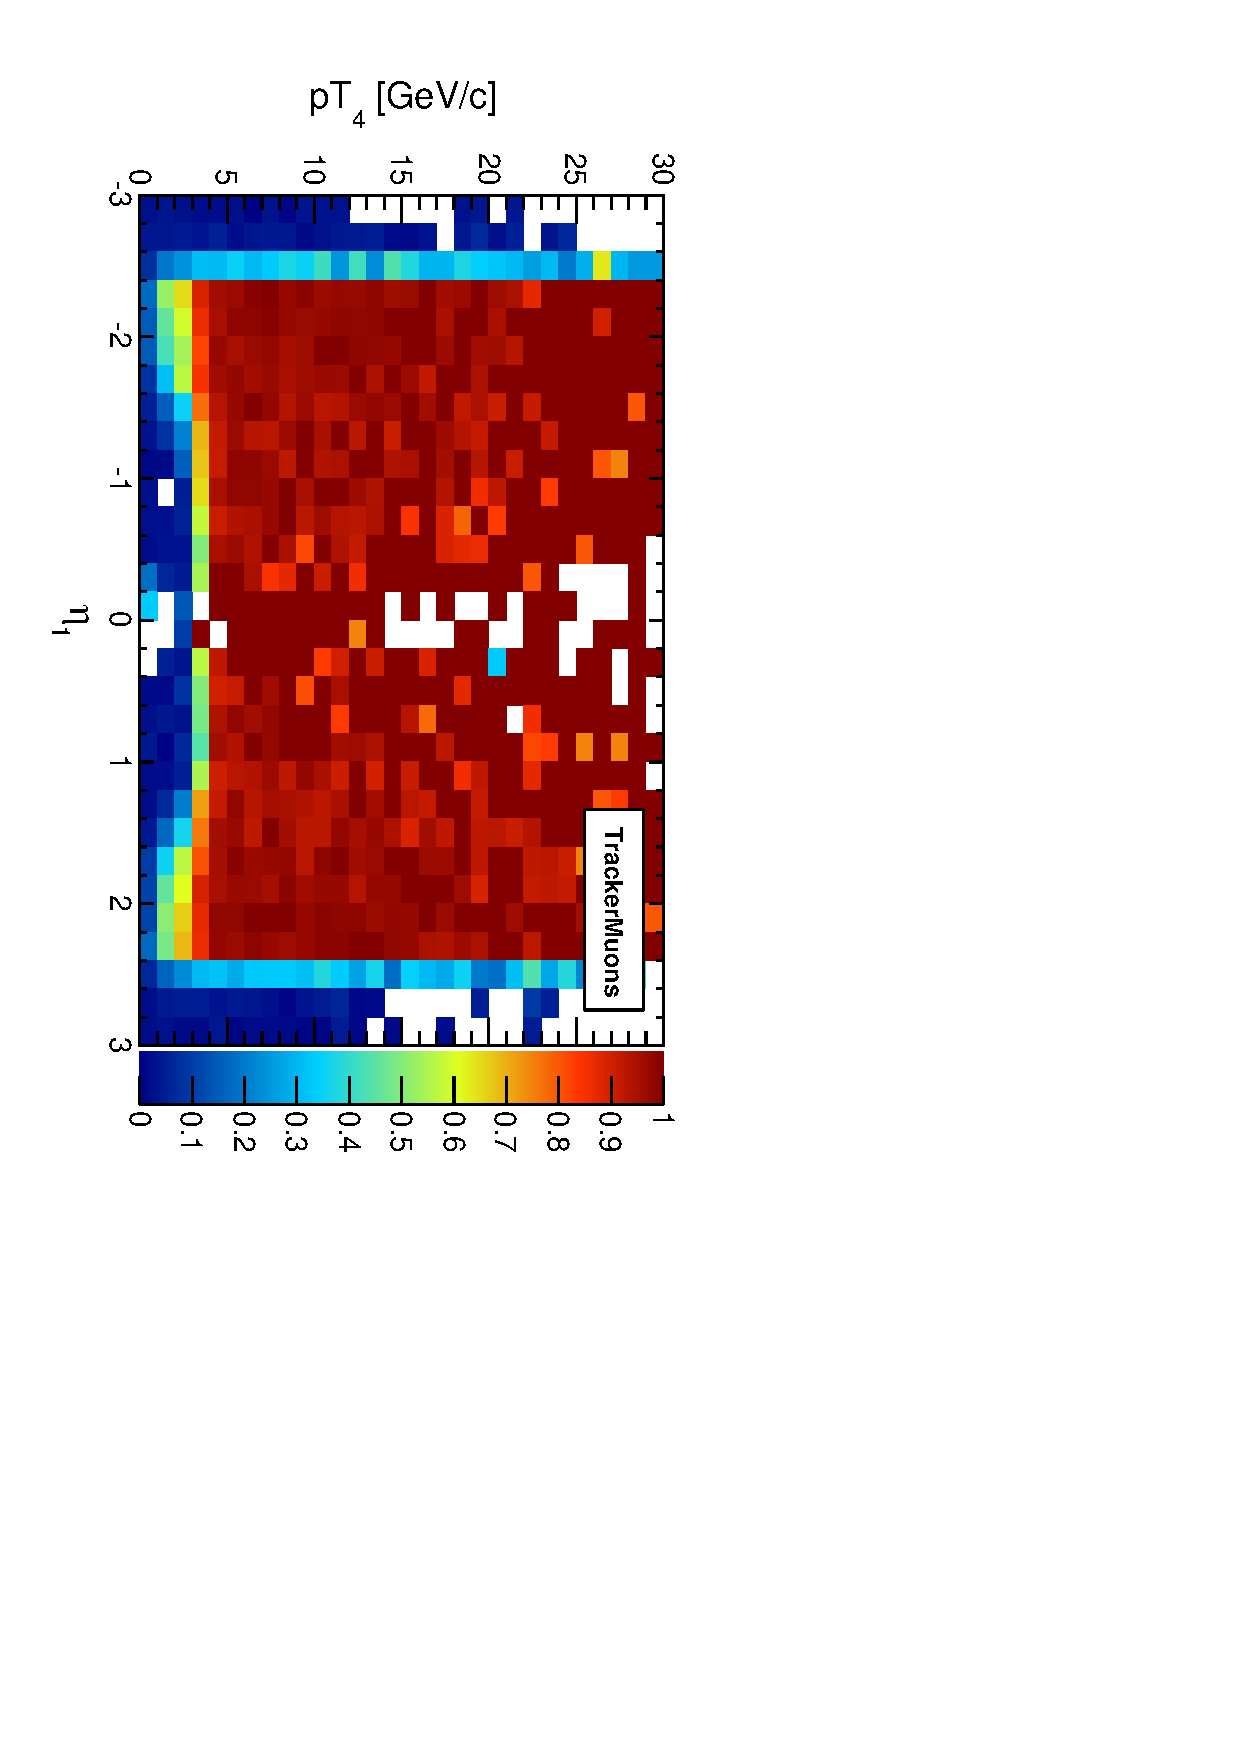
\includegraphics[height=0.5\linewidth, angle=90]{fig/acceptance3_plot/pt4vseta1_TrackerMuons.pdf}
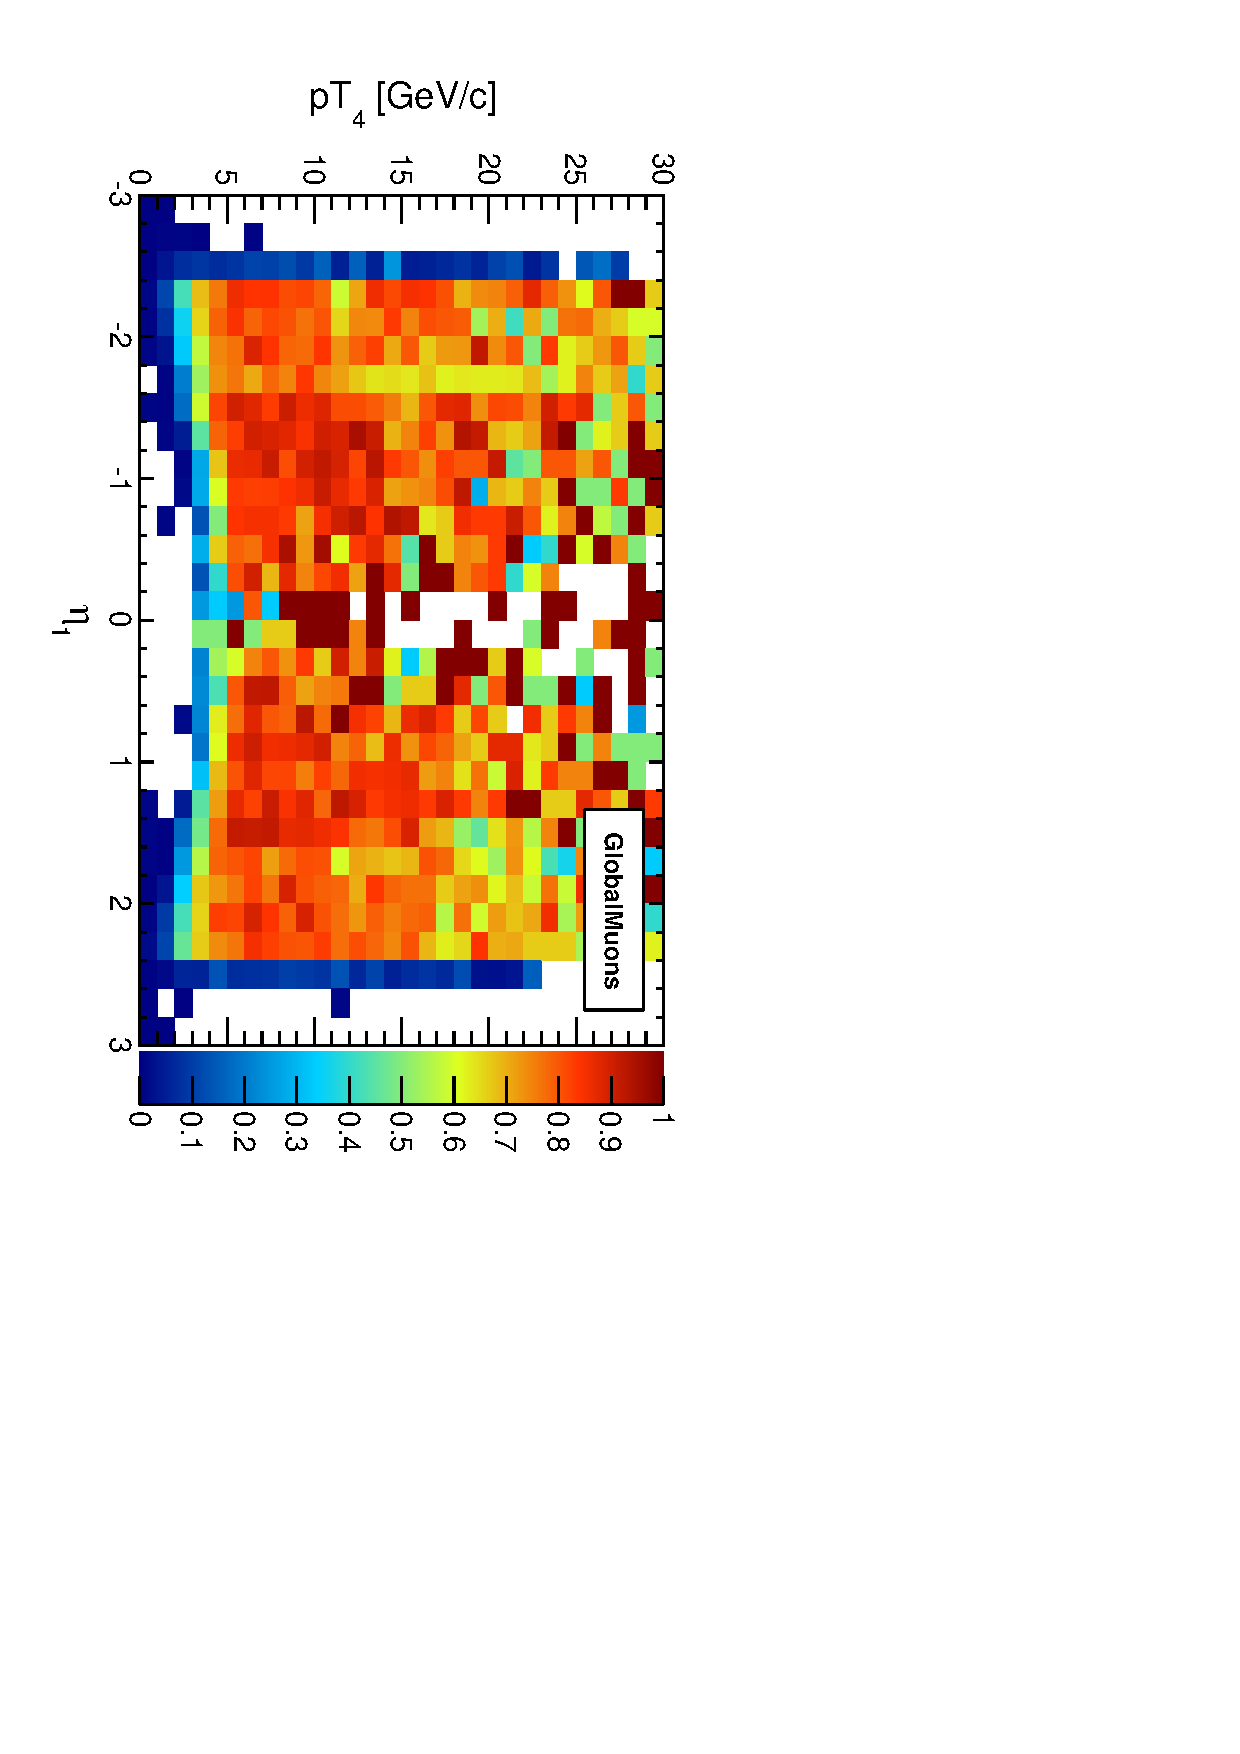
\includegraphics[height=0.5\linewidth, angle=90]{fig/acceptance3_plot/pt4vseta1_GlobalMuons.pdf}

\caption{Acceptance region and efficiency for four muons.  $pT_4$ is
  the fourth-highest $p_T$ muon in the event, $\eta_1$ is the
  largest-magnitude pseudorapidity in the event.  Denominator: all
  generated events; numerator: events with four reconstructed
  muons. \label{fig:pt4vseta1}}
\end{figure}

\subsection{Efficiency of track-reconstruction}

GlobalMuons require StandAloneMuons

Overlapping muons in muon system can confuse StandAloneMuon-finding algorithm

GlobalMuon efficiency is less than or equal to StandAloneMuon
efficiency, because the global algorithm requires a StandAloneMuon.
This is not evident in the plots that require an MC match (because of
the StandAloneMuon resolution), but it is evident in the plots that
only require two reconstructed muons.

\begin{figure}[p]
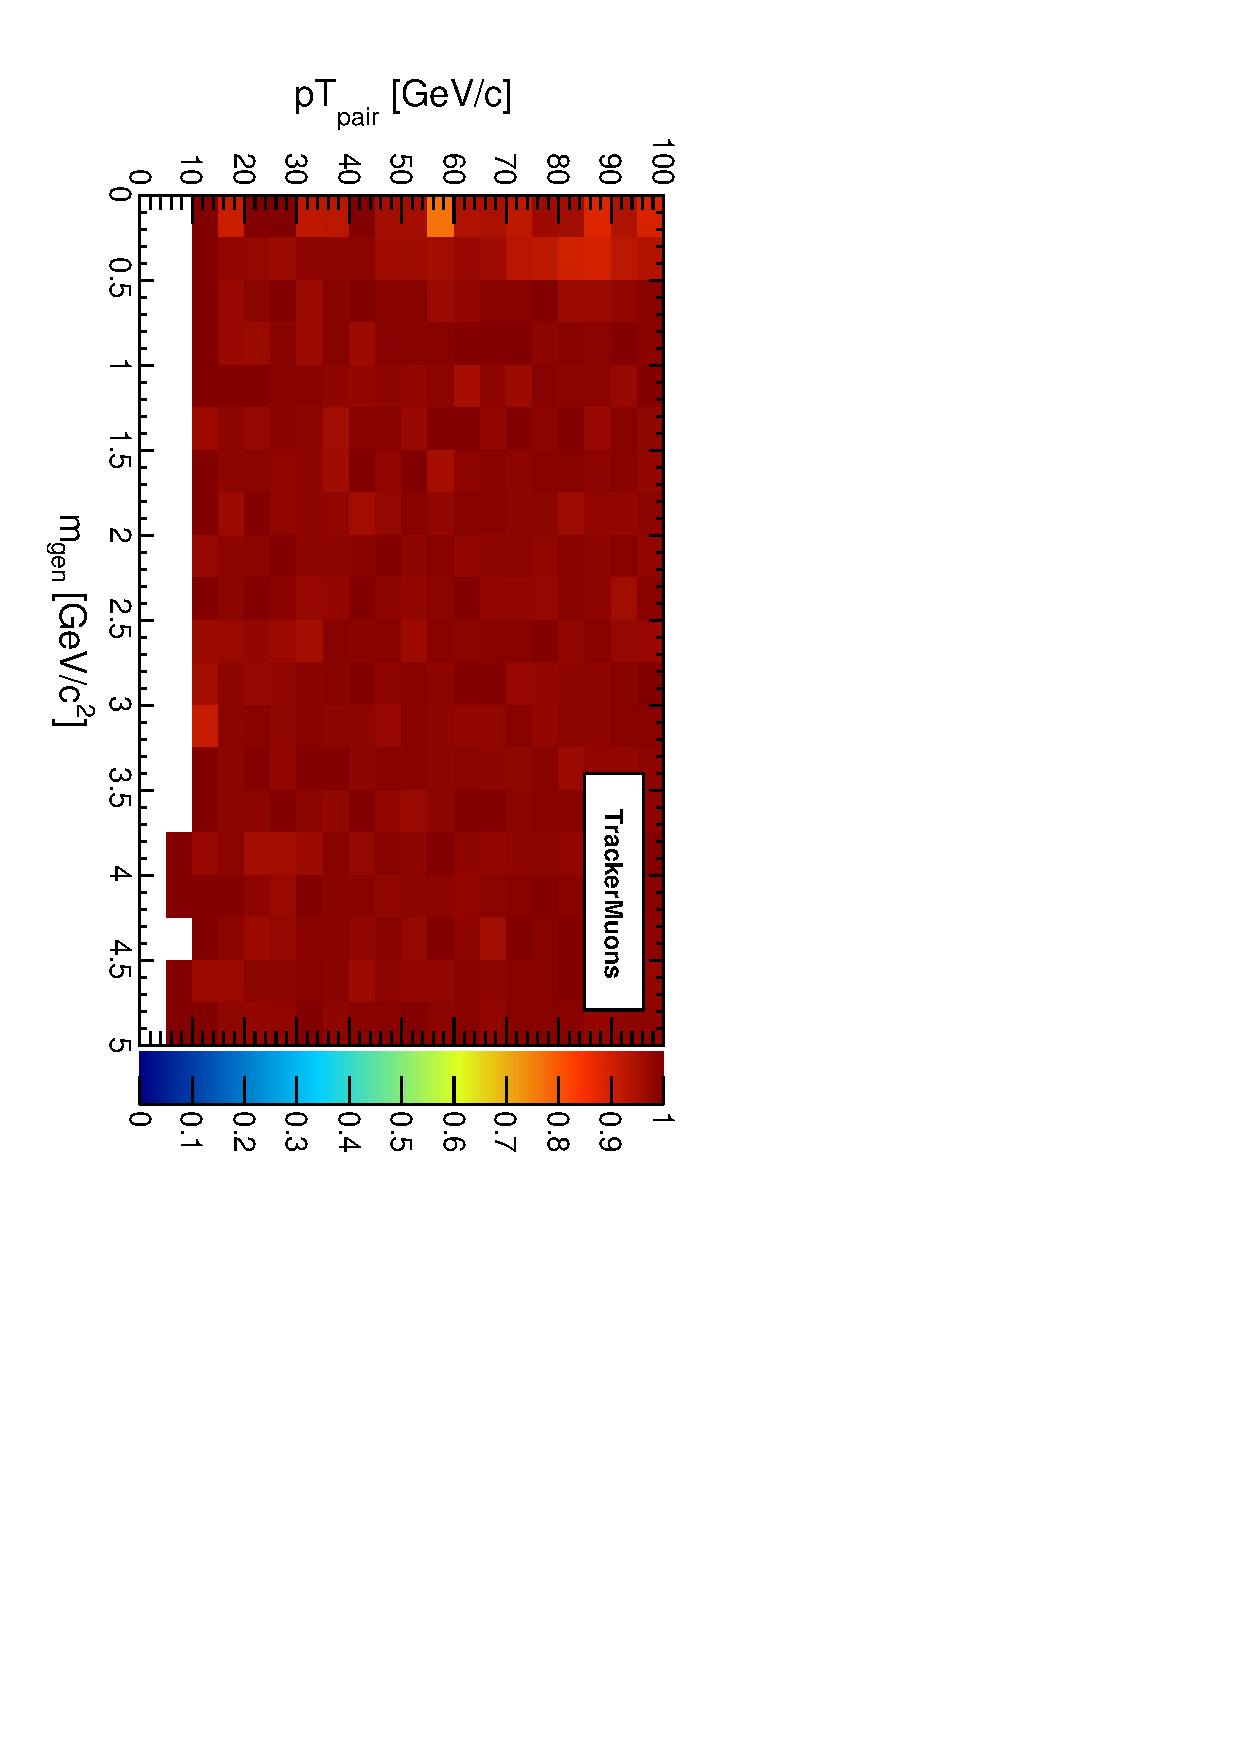
\includegraphics[height=0.5\linewidth, angle=90]{fig/acceptance_plot/pairptvsmass_TrackerMuons.pdf}
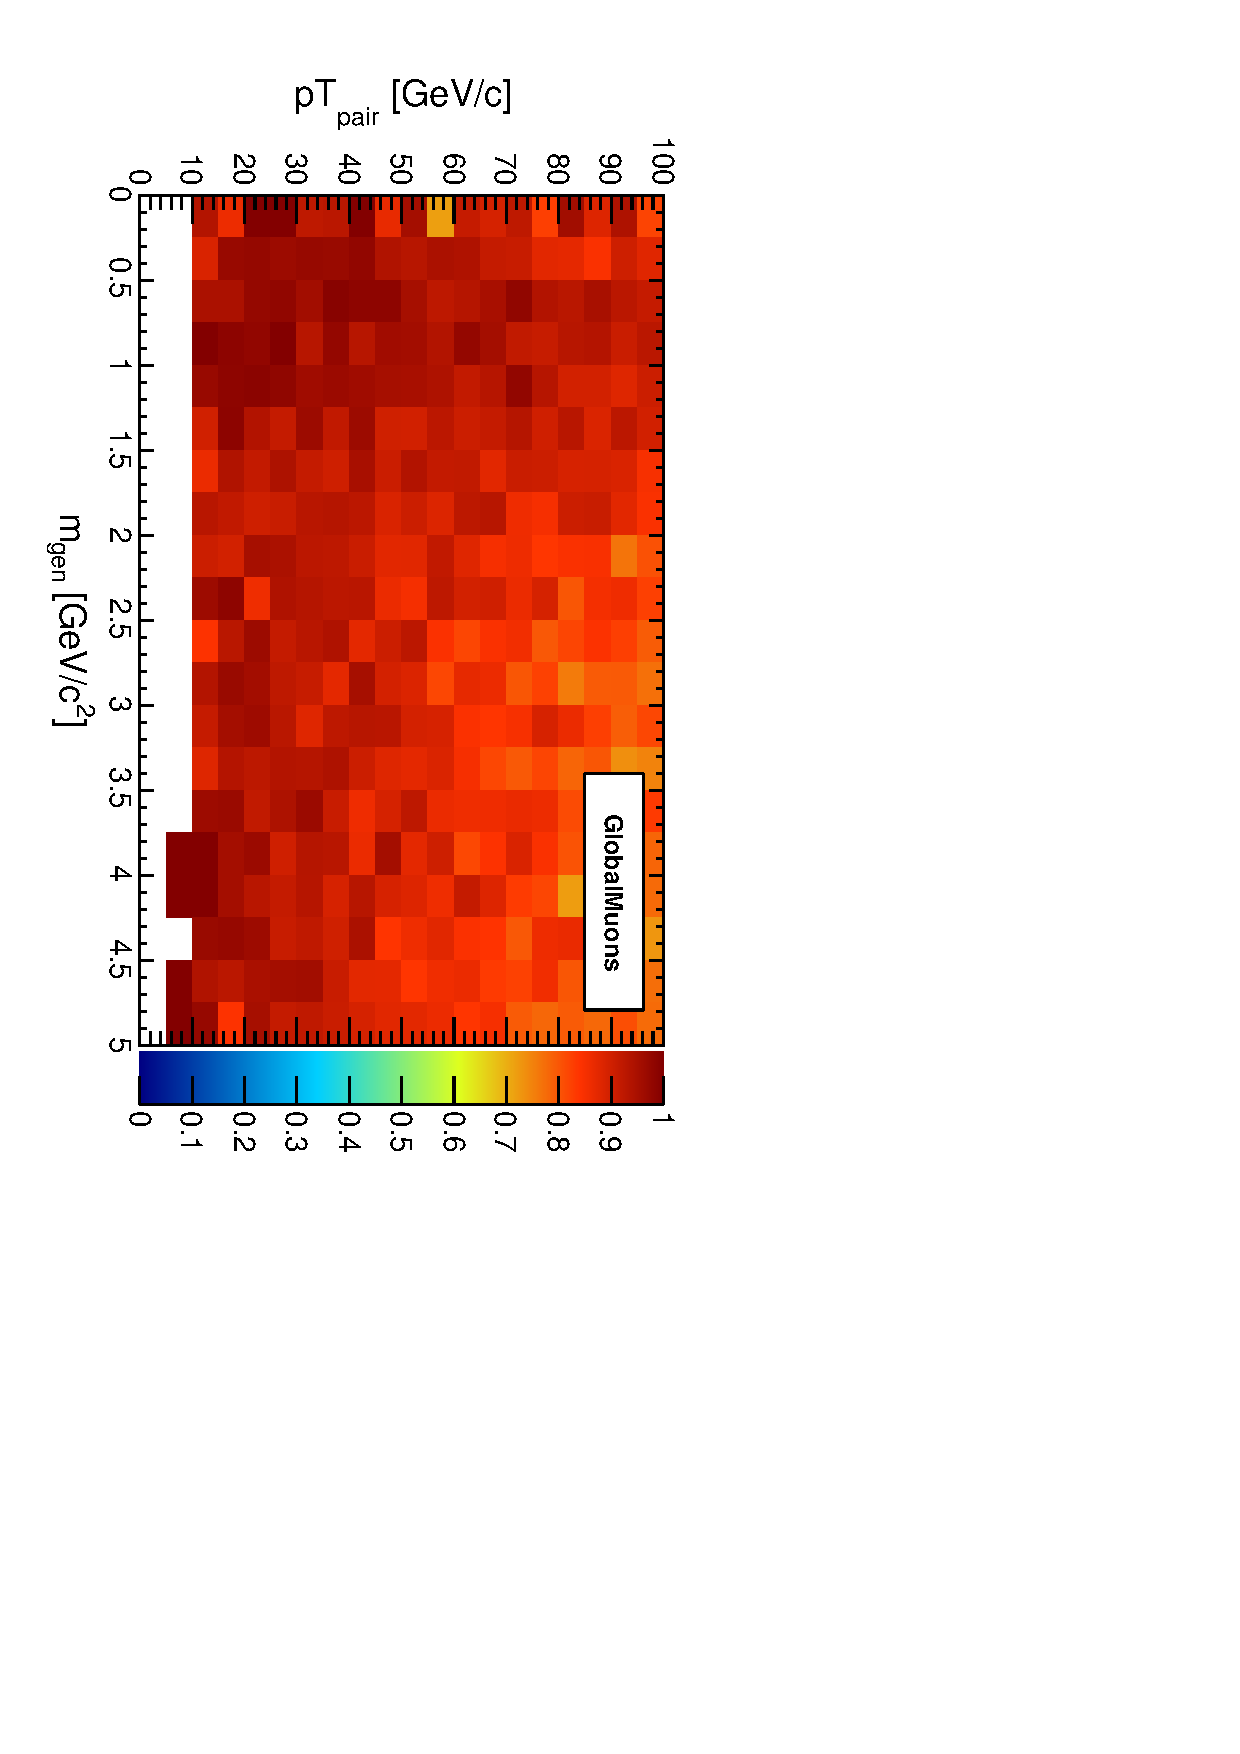
\includegraphics[height=0.5\linewidth, angle=90]{fig/acceptance_plot/pairptvsmass_GlobalMuons.pdf}

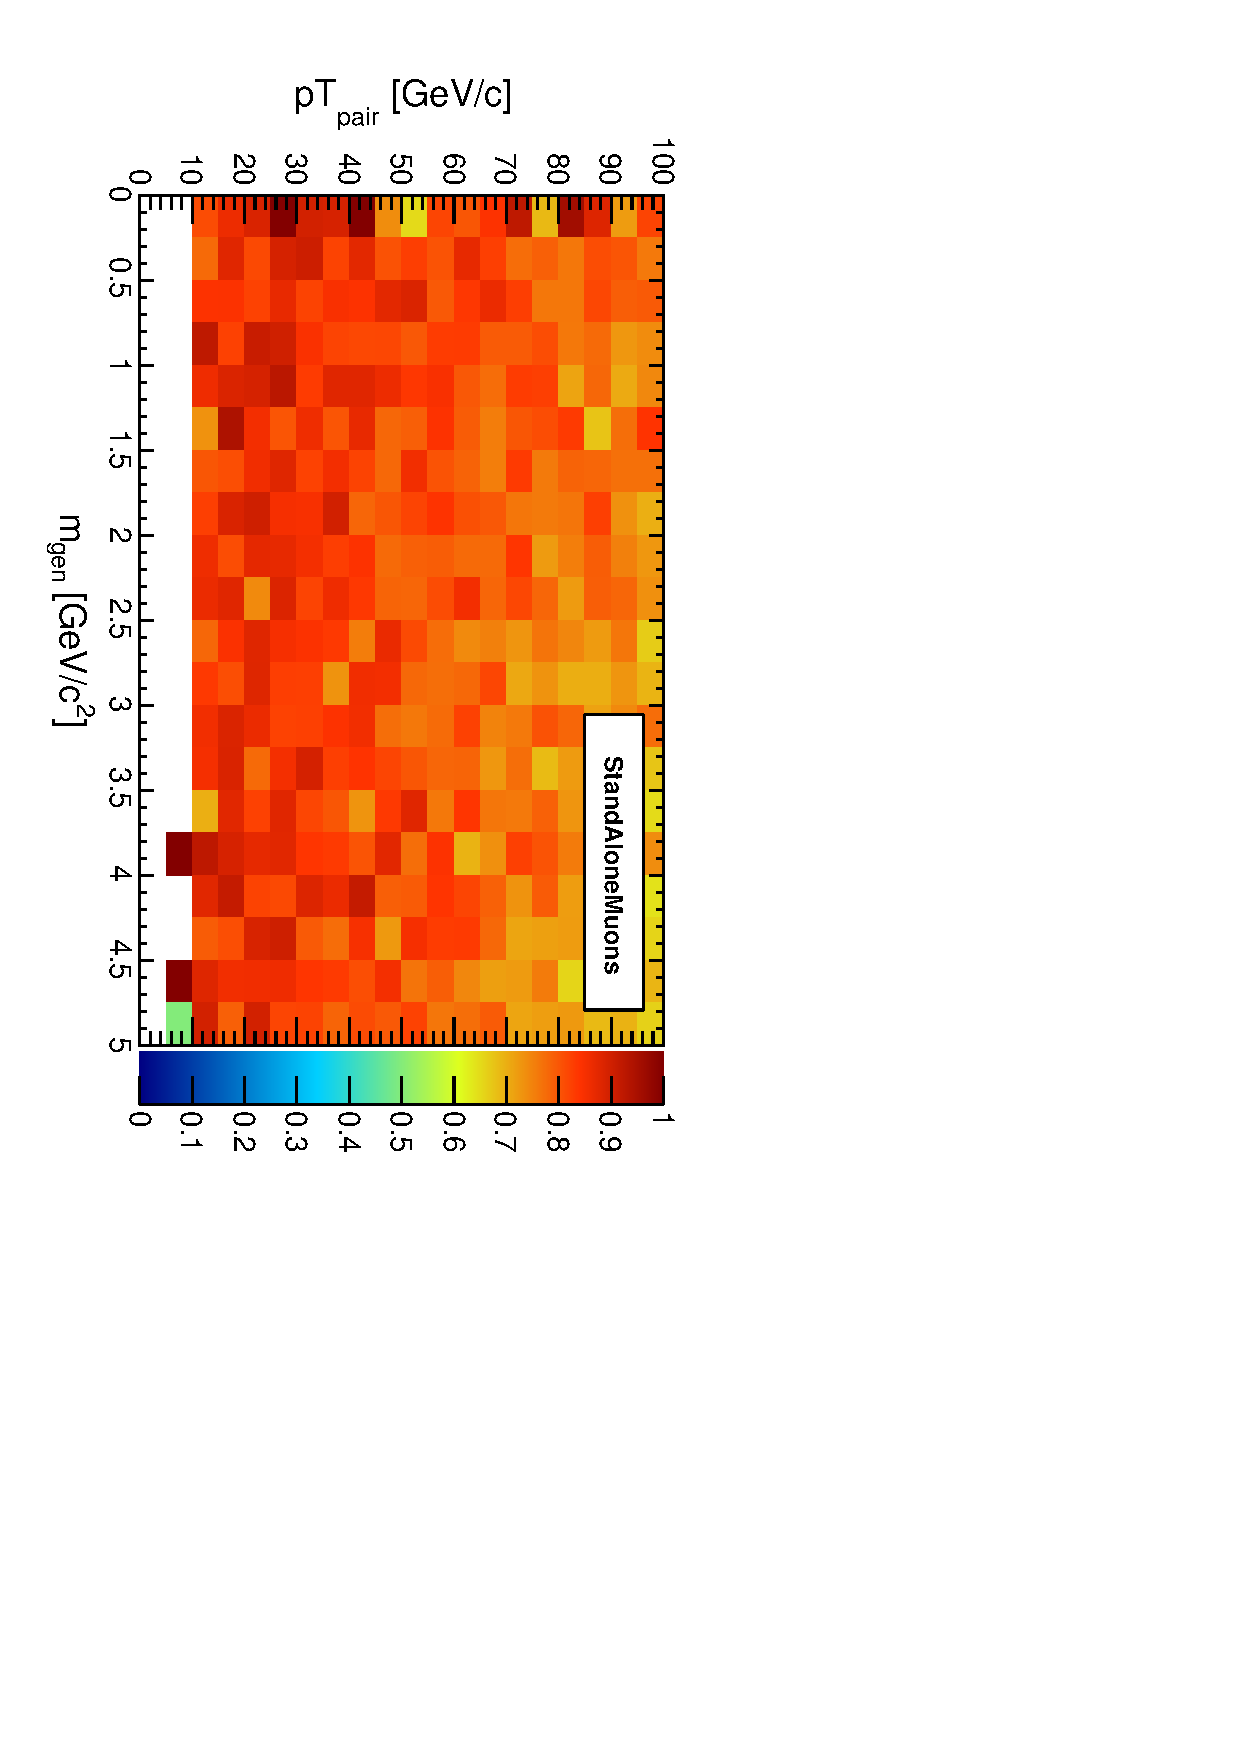
\includegraphics[height=0.5\linewidth, angle=90]{fig/acceptance_plot/pairptvsmass_StandAloneUpdatedDefault.pdf}
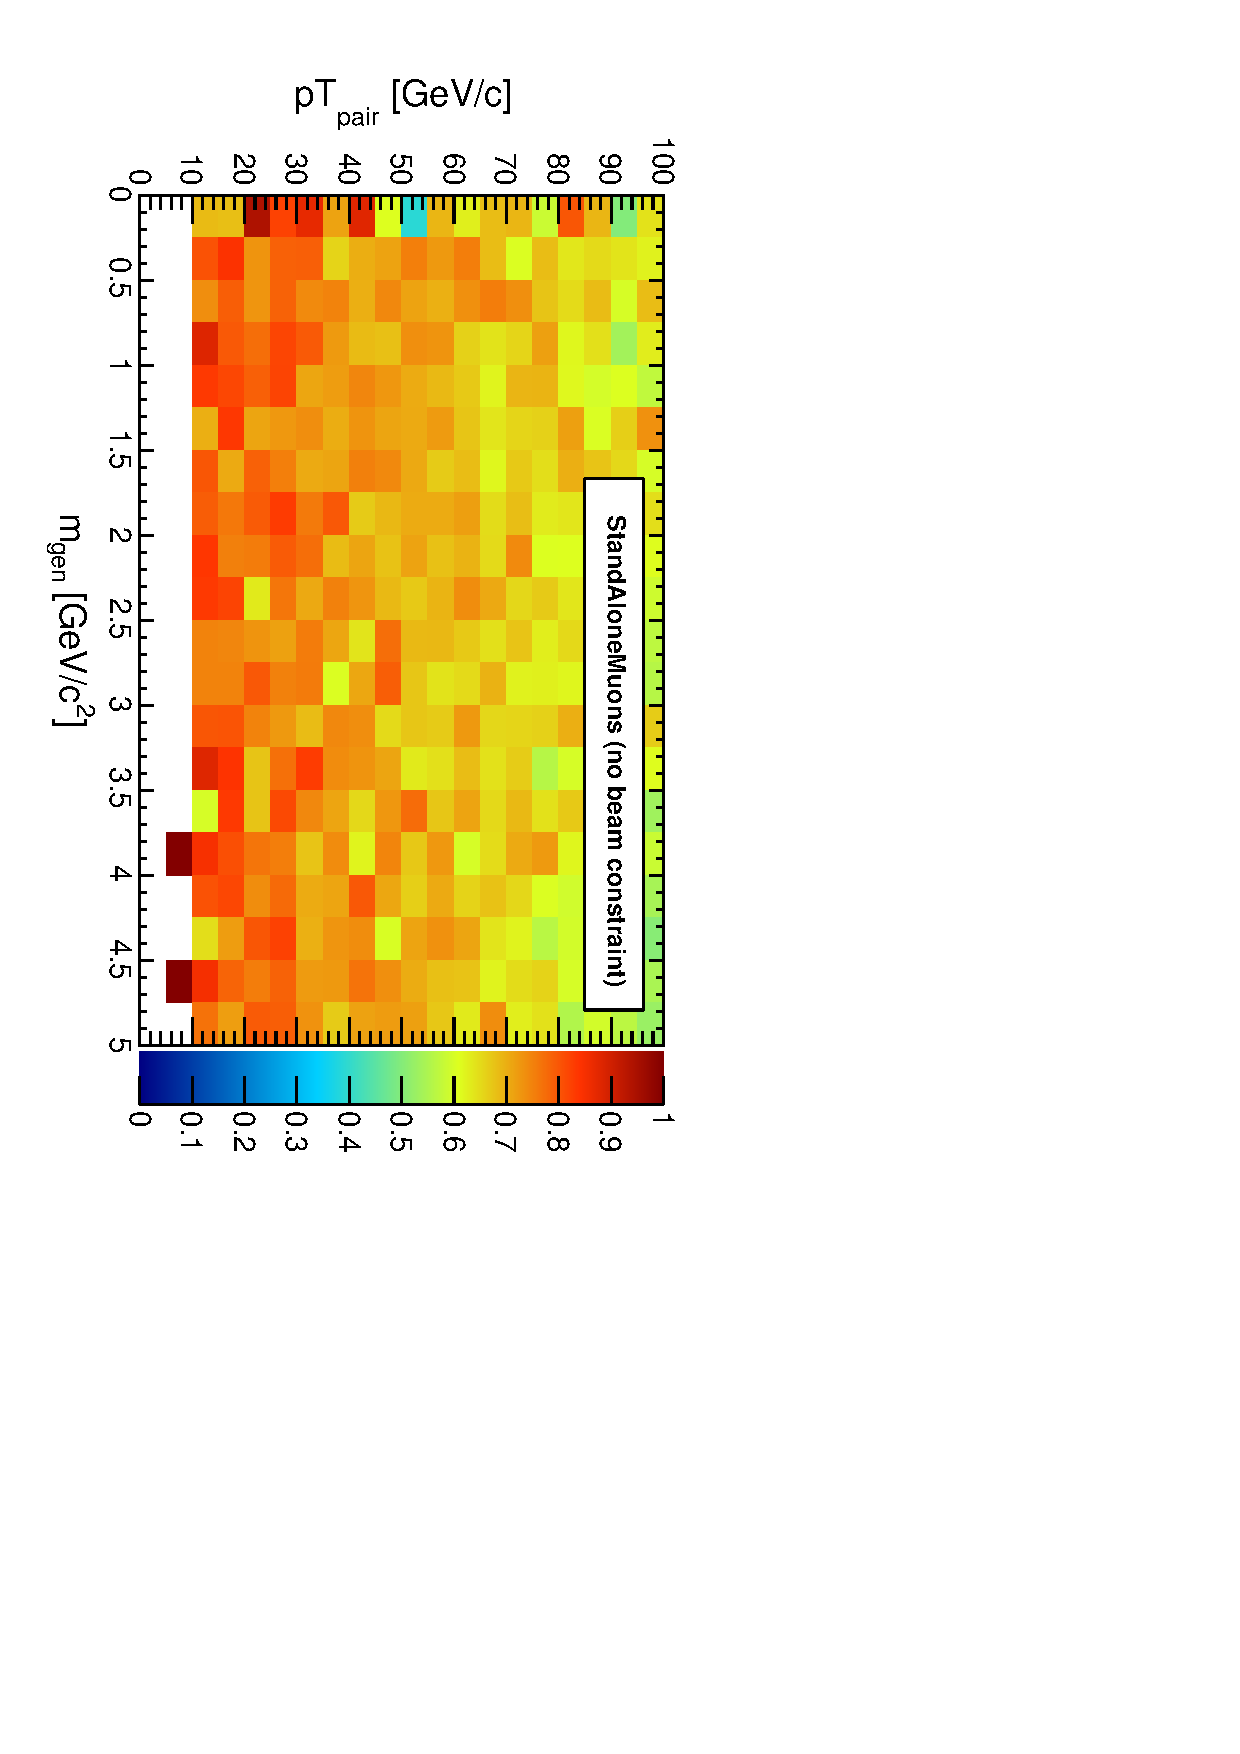
\includegraphics[height=0.5\linewidth, angle=90]{fig/acceptance_plot/pairptvsmass_StandAloneDefault.pdf}

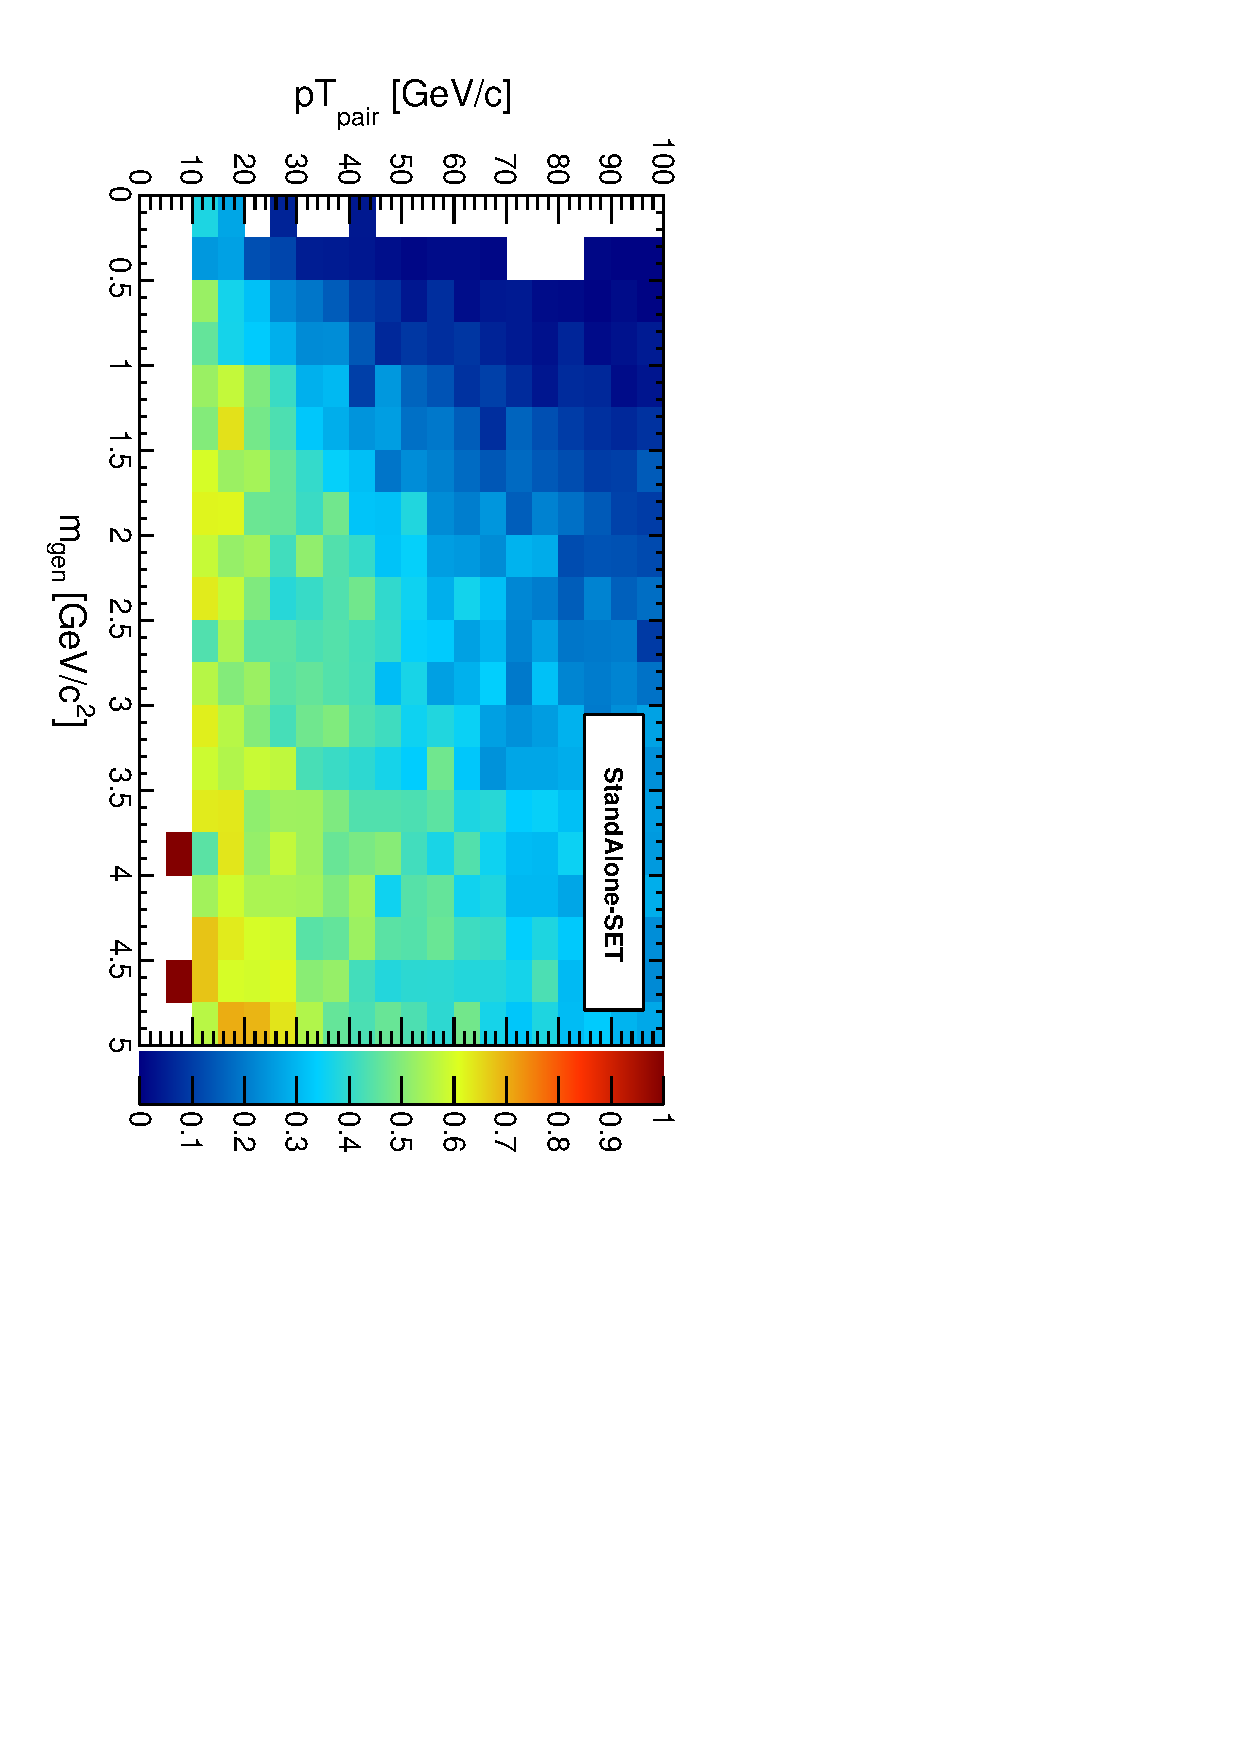
\includegraphics[height=0.5\linewidth, angle=90]{fig/acceptance_plot/pairptvsmass_StandAloneUpdatedSET.pdf}
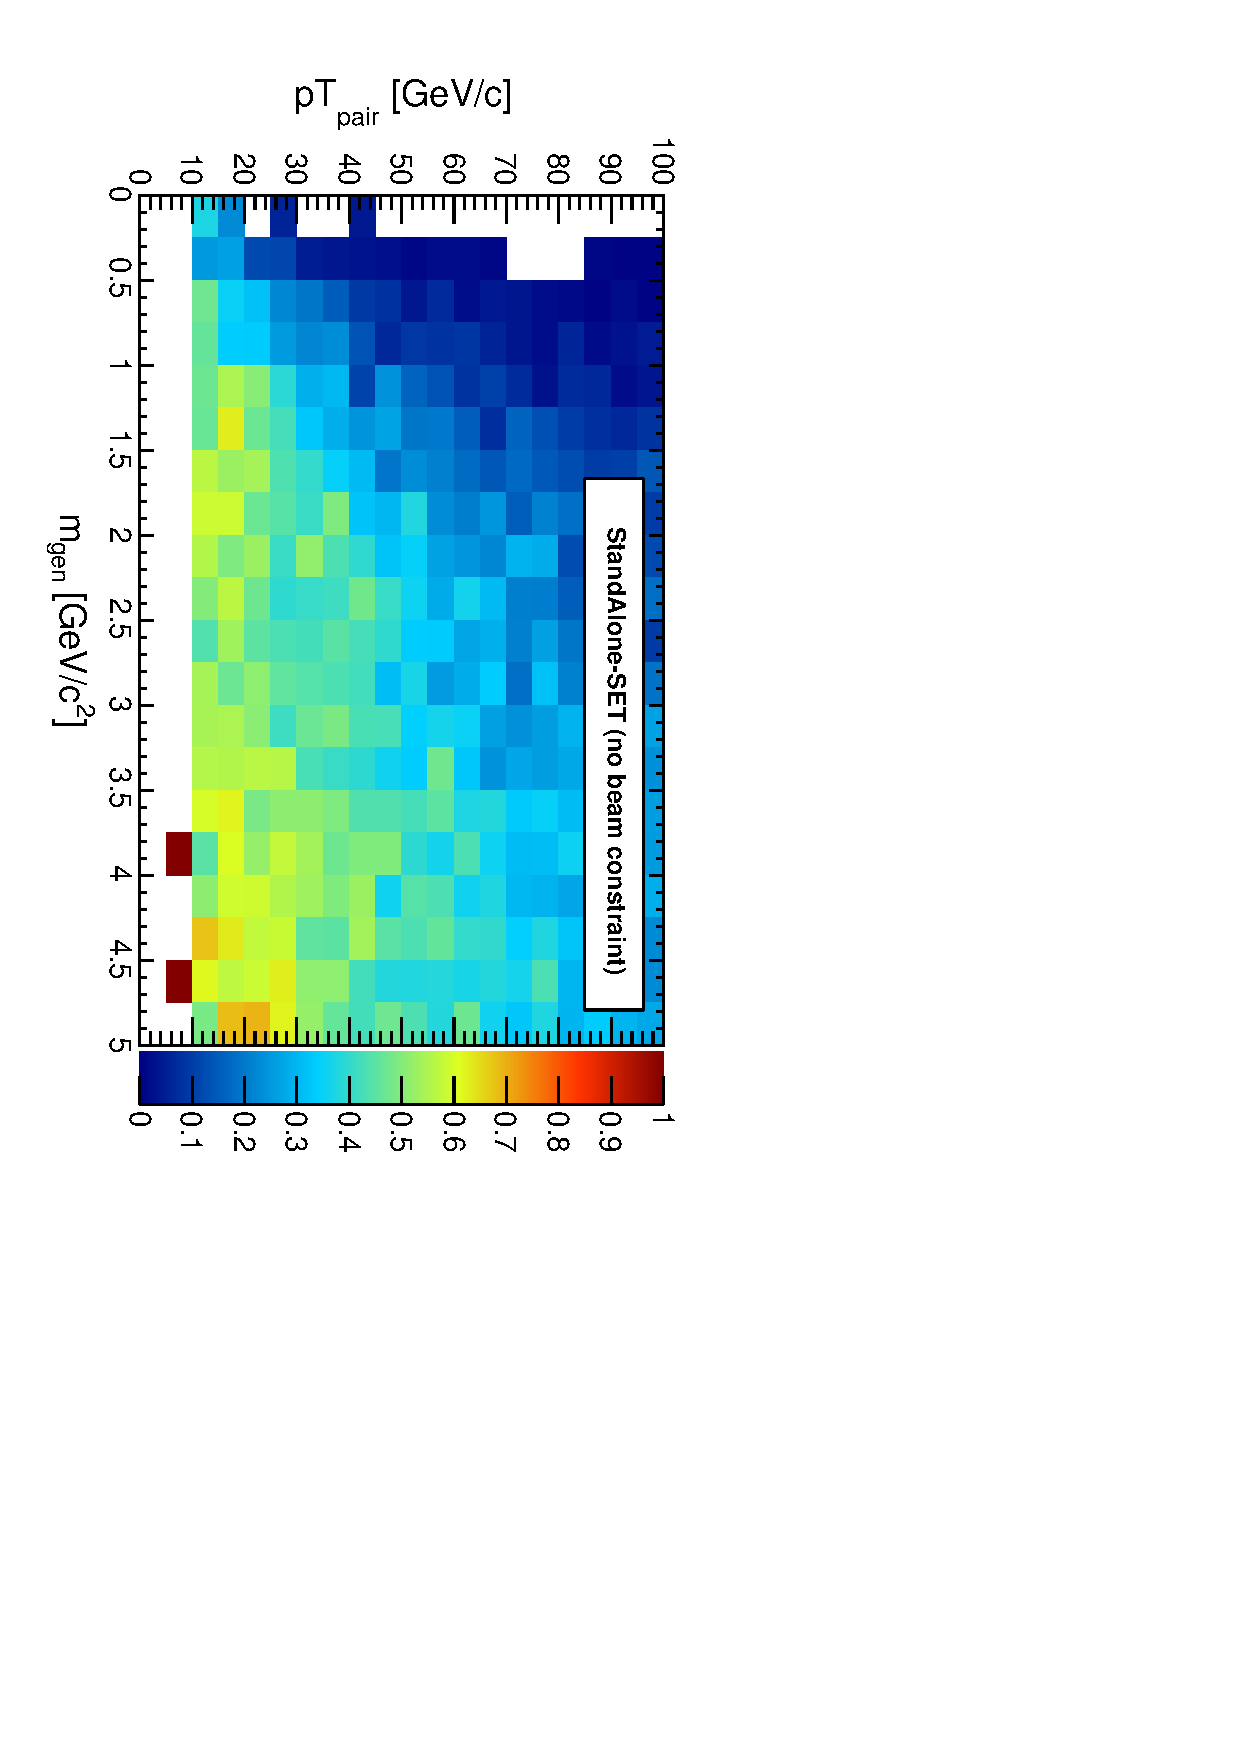
\includegraphics[height=0.5\linewidth, angle=90]{fig/acceptance_plot/pairptvsmass_StandAloneSET.pdf}

\caption{Efficiency as a function of physics-relevant variables: $p_T$
  and invariant mass of the $\mu^+$-$\mu^-$ pair.  Denominator:
  generated events with $pT_2 > 5$~GeV/$c$ and $|\eta_1| < 2.4$;
  numerator: reconstructed and MC-matched $\mu^+$ and
  $\mu^-$. \label{fig:pairptvsmass}}
\end{figure}

\begin{figure}[p]
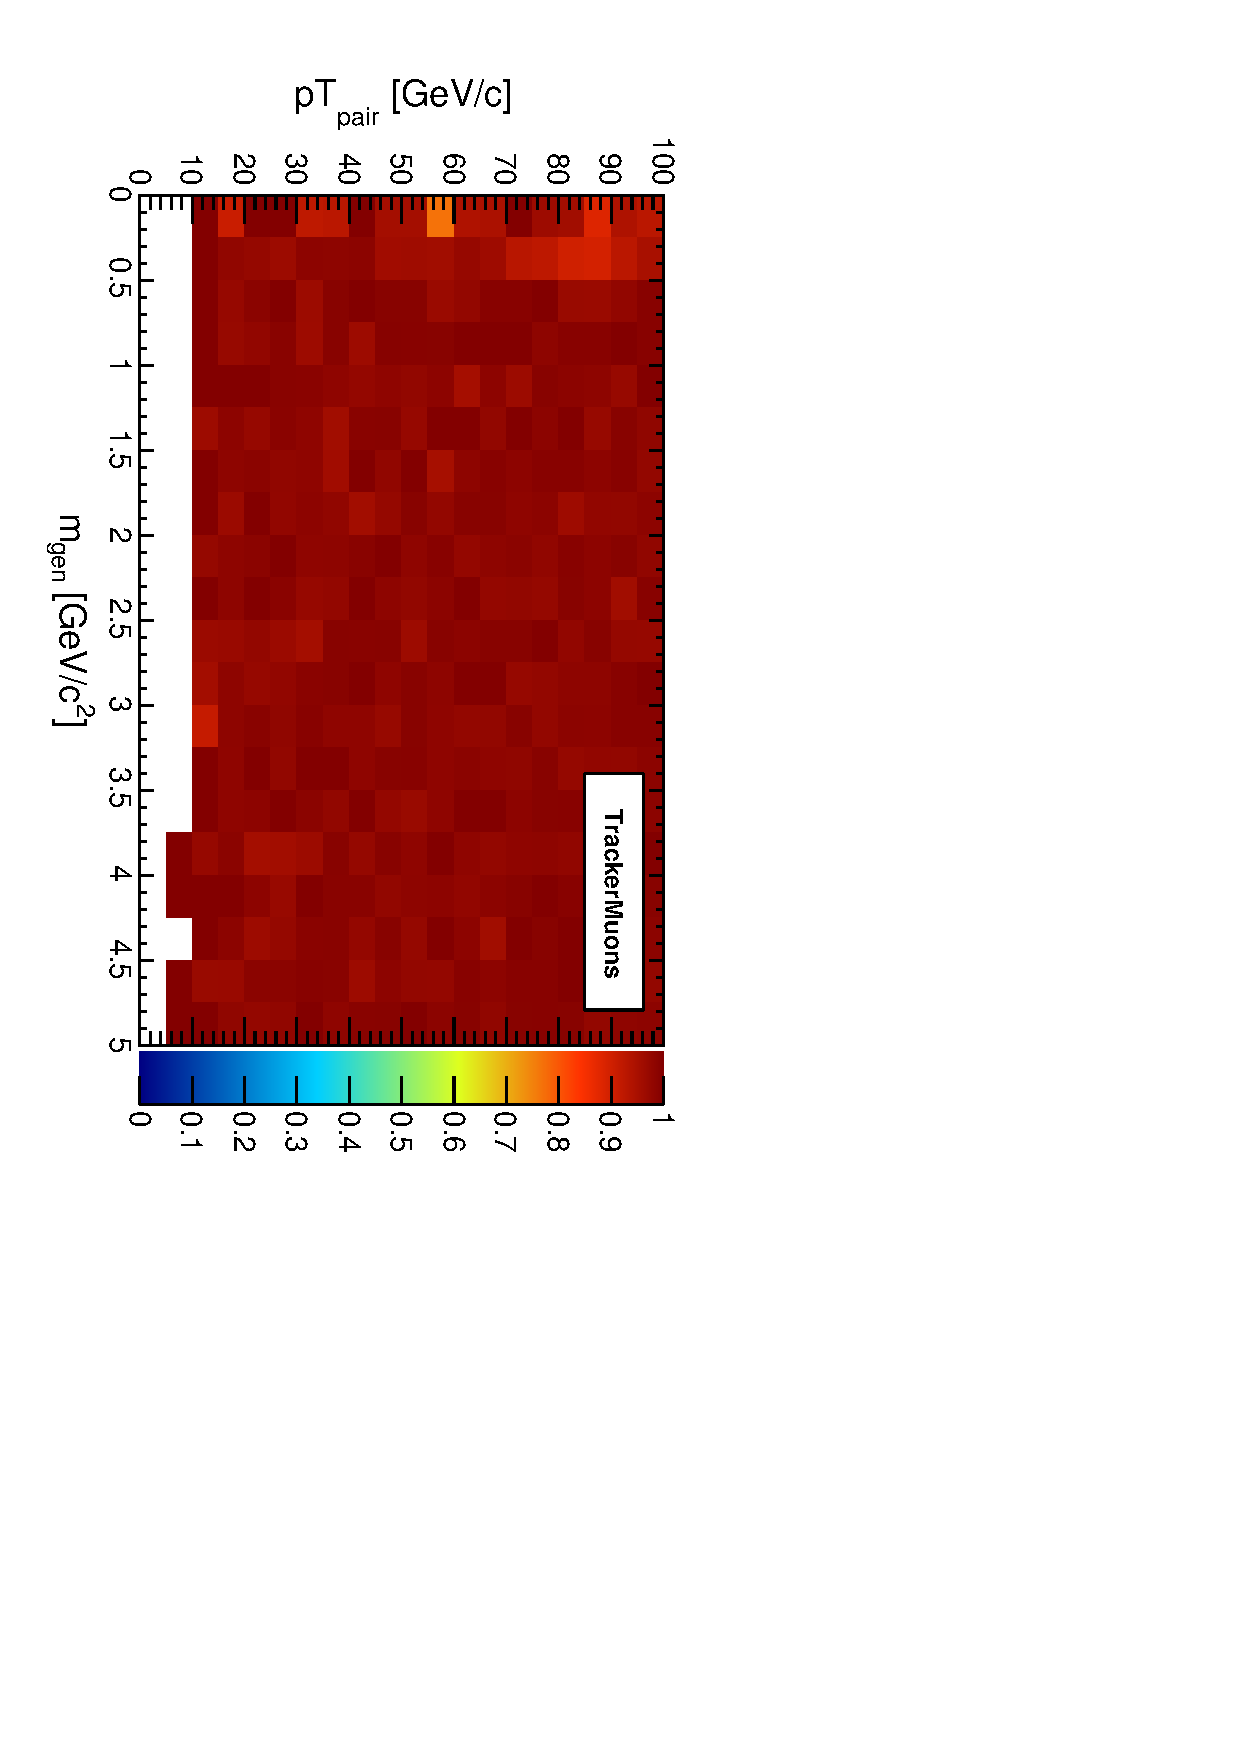
\includegraphics[height=0.5\linewidth, angle=90]{fig/acceptanceNoMCMatch_plot/pairptvsmass_TrackerMuons.pdf}
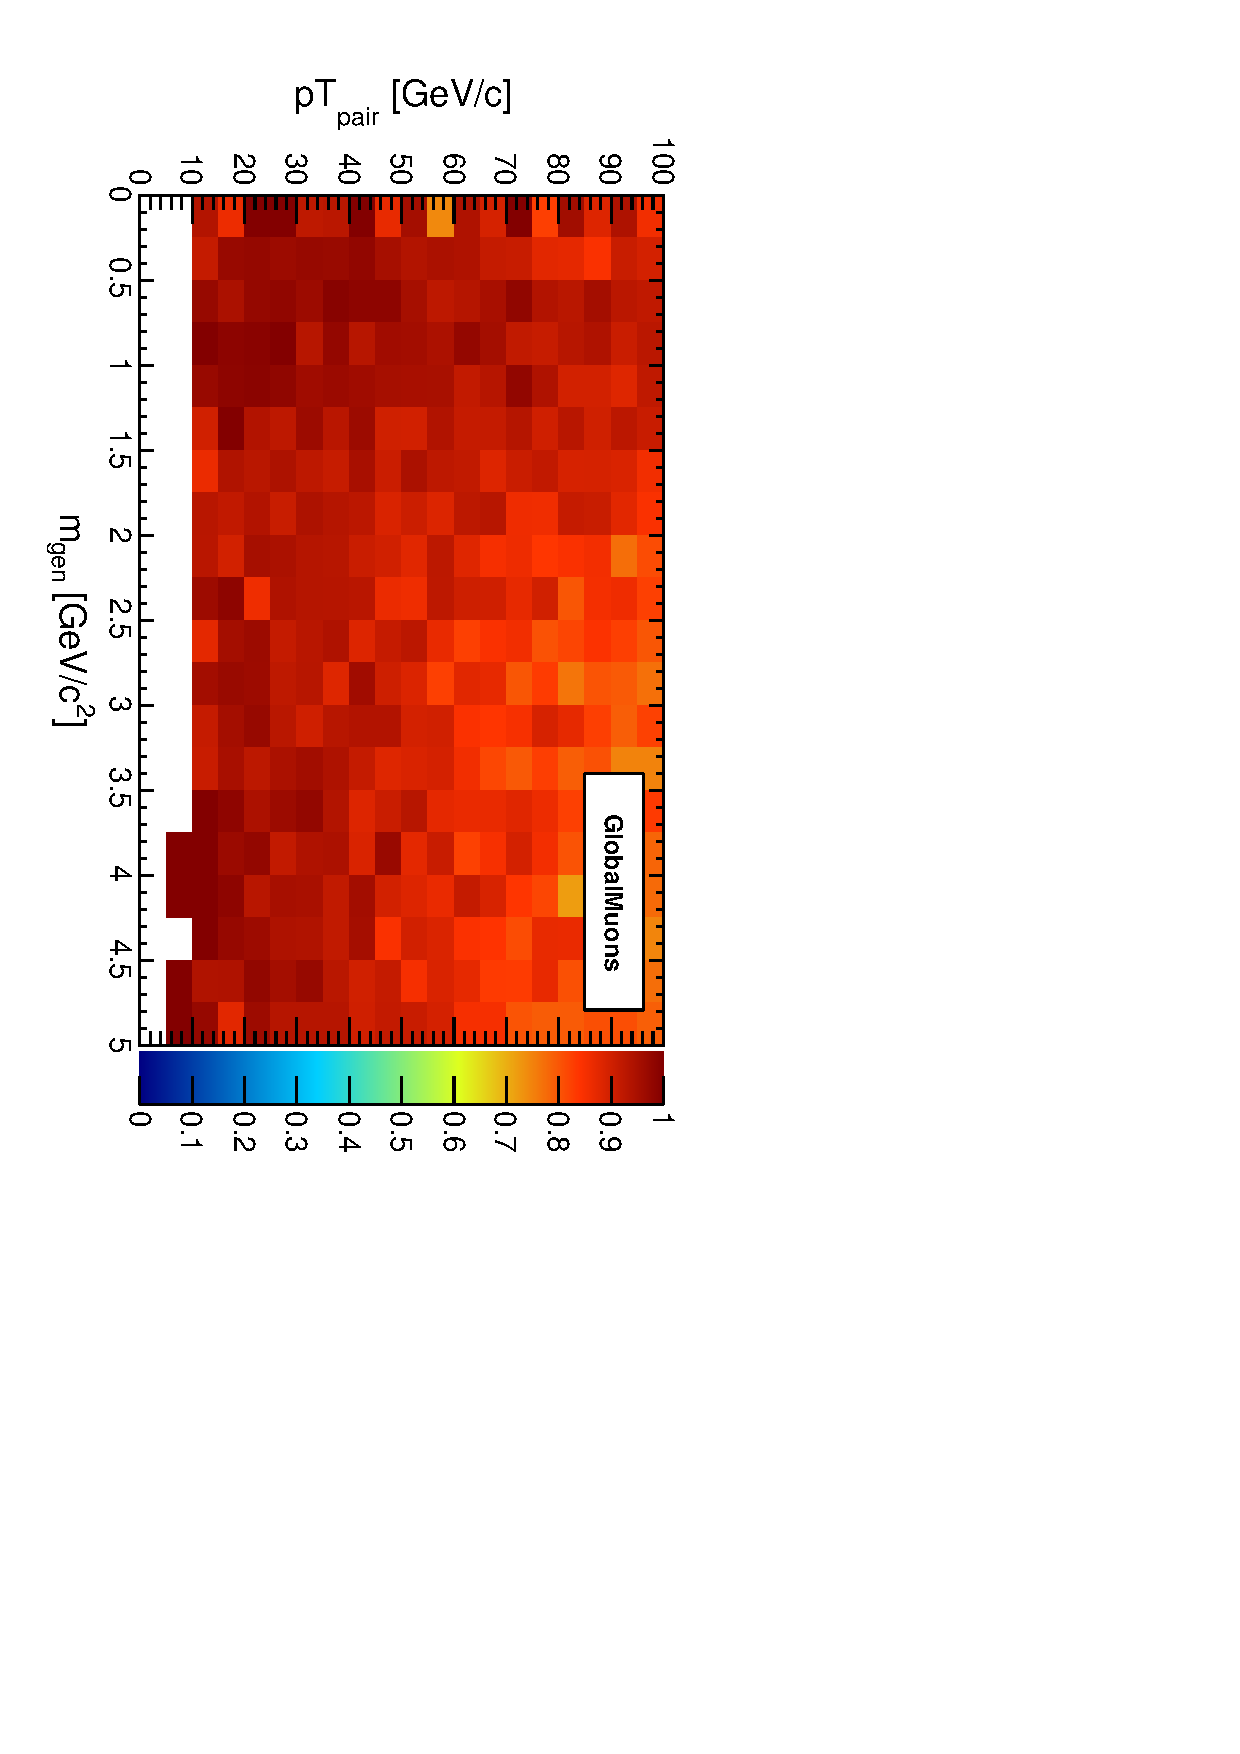
\includegraphics[height=0.5\linewidth, angle=90]{fig/acceptanceNoMCMatch_plot/pairptvsmass_GlobalMuons.pdf}

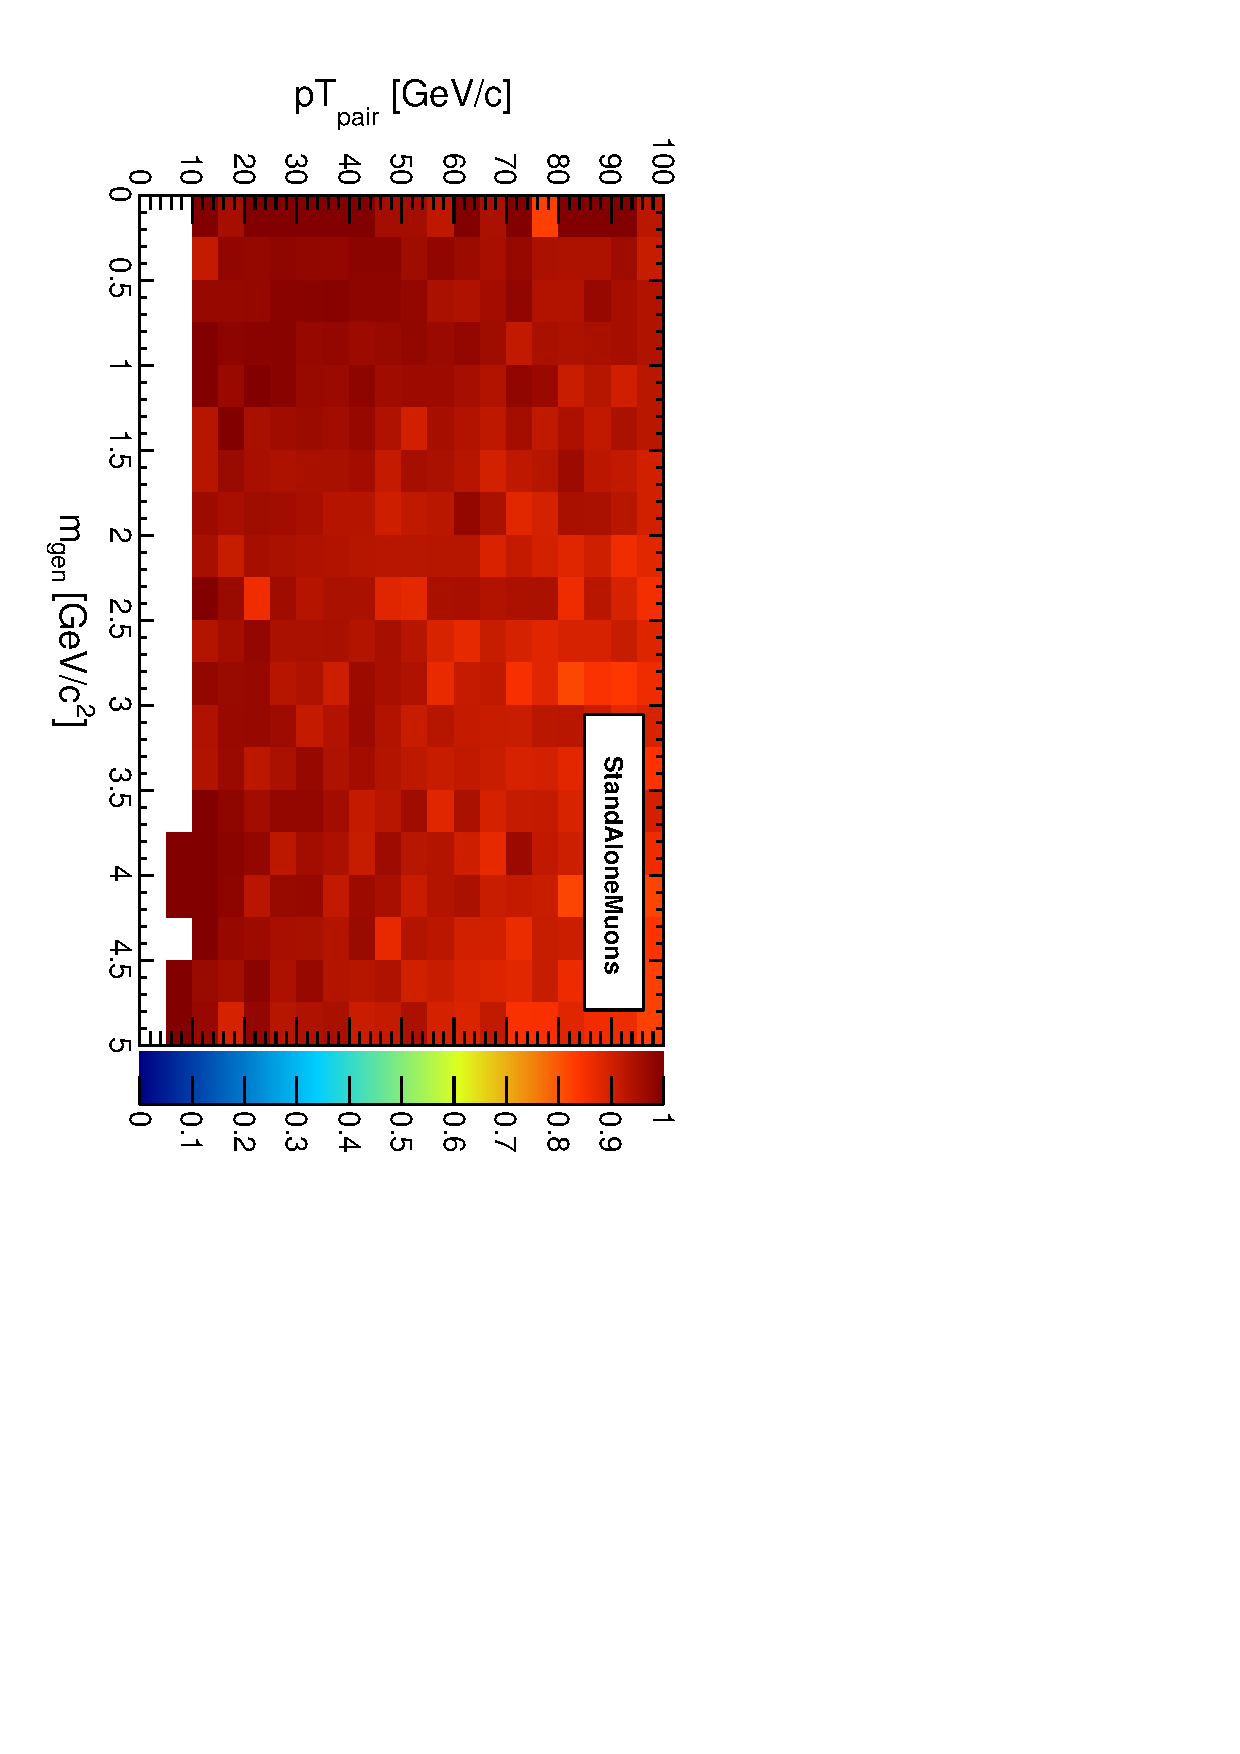
\includegraphics[height=0.5\linewidth, angle=90]{fig/acceptanceNoMCMatch_plot/pairptvsmass_StandAloneUpdatedDefault.pdf}
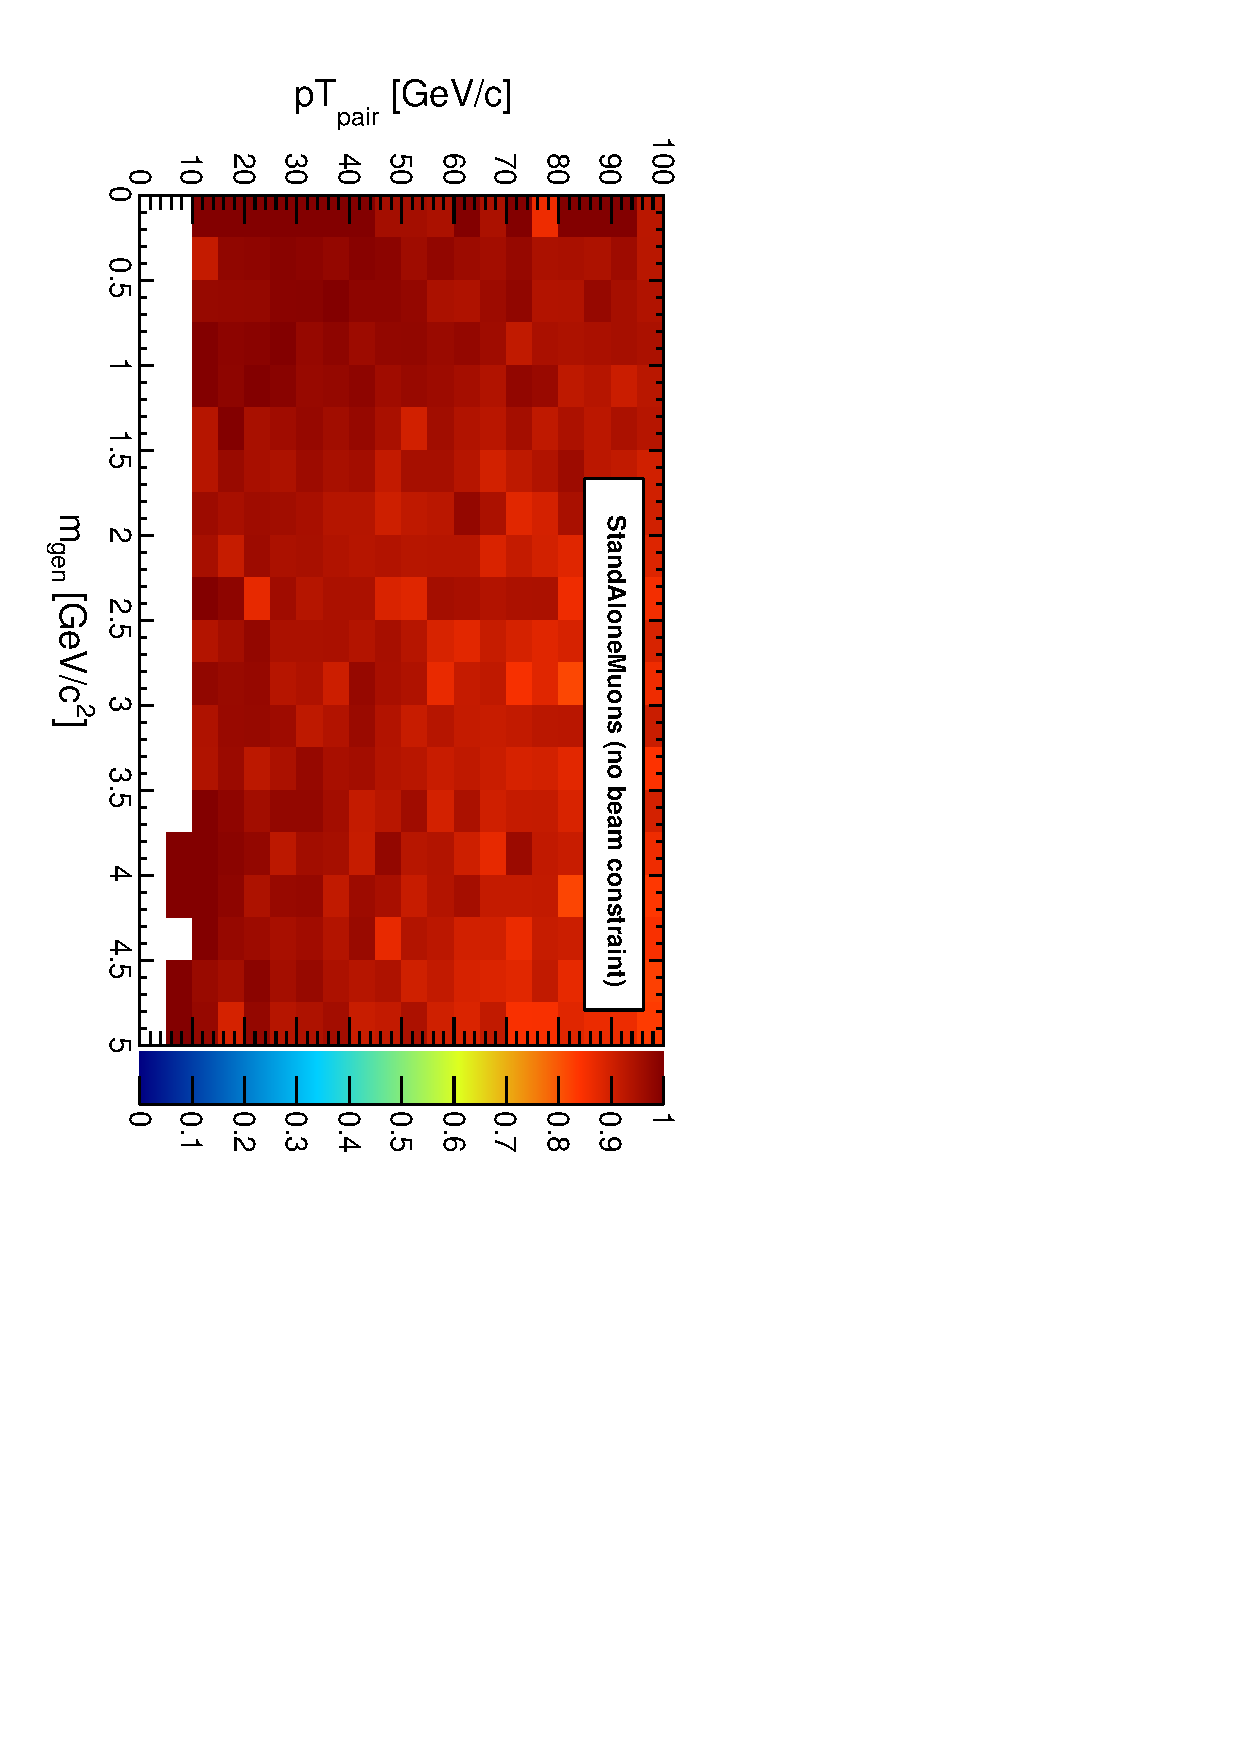
\includegraphics[height=0.5\linewidth, angle=90]{fig/acceptanceNoMCMatch_plot/pairptvsmass_StandAloneDefault.pdf}

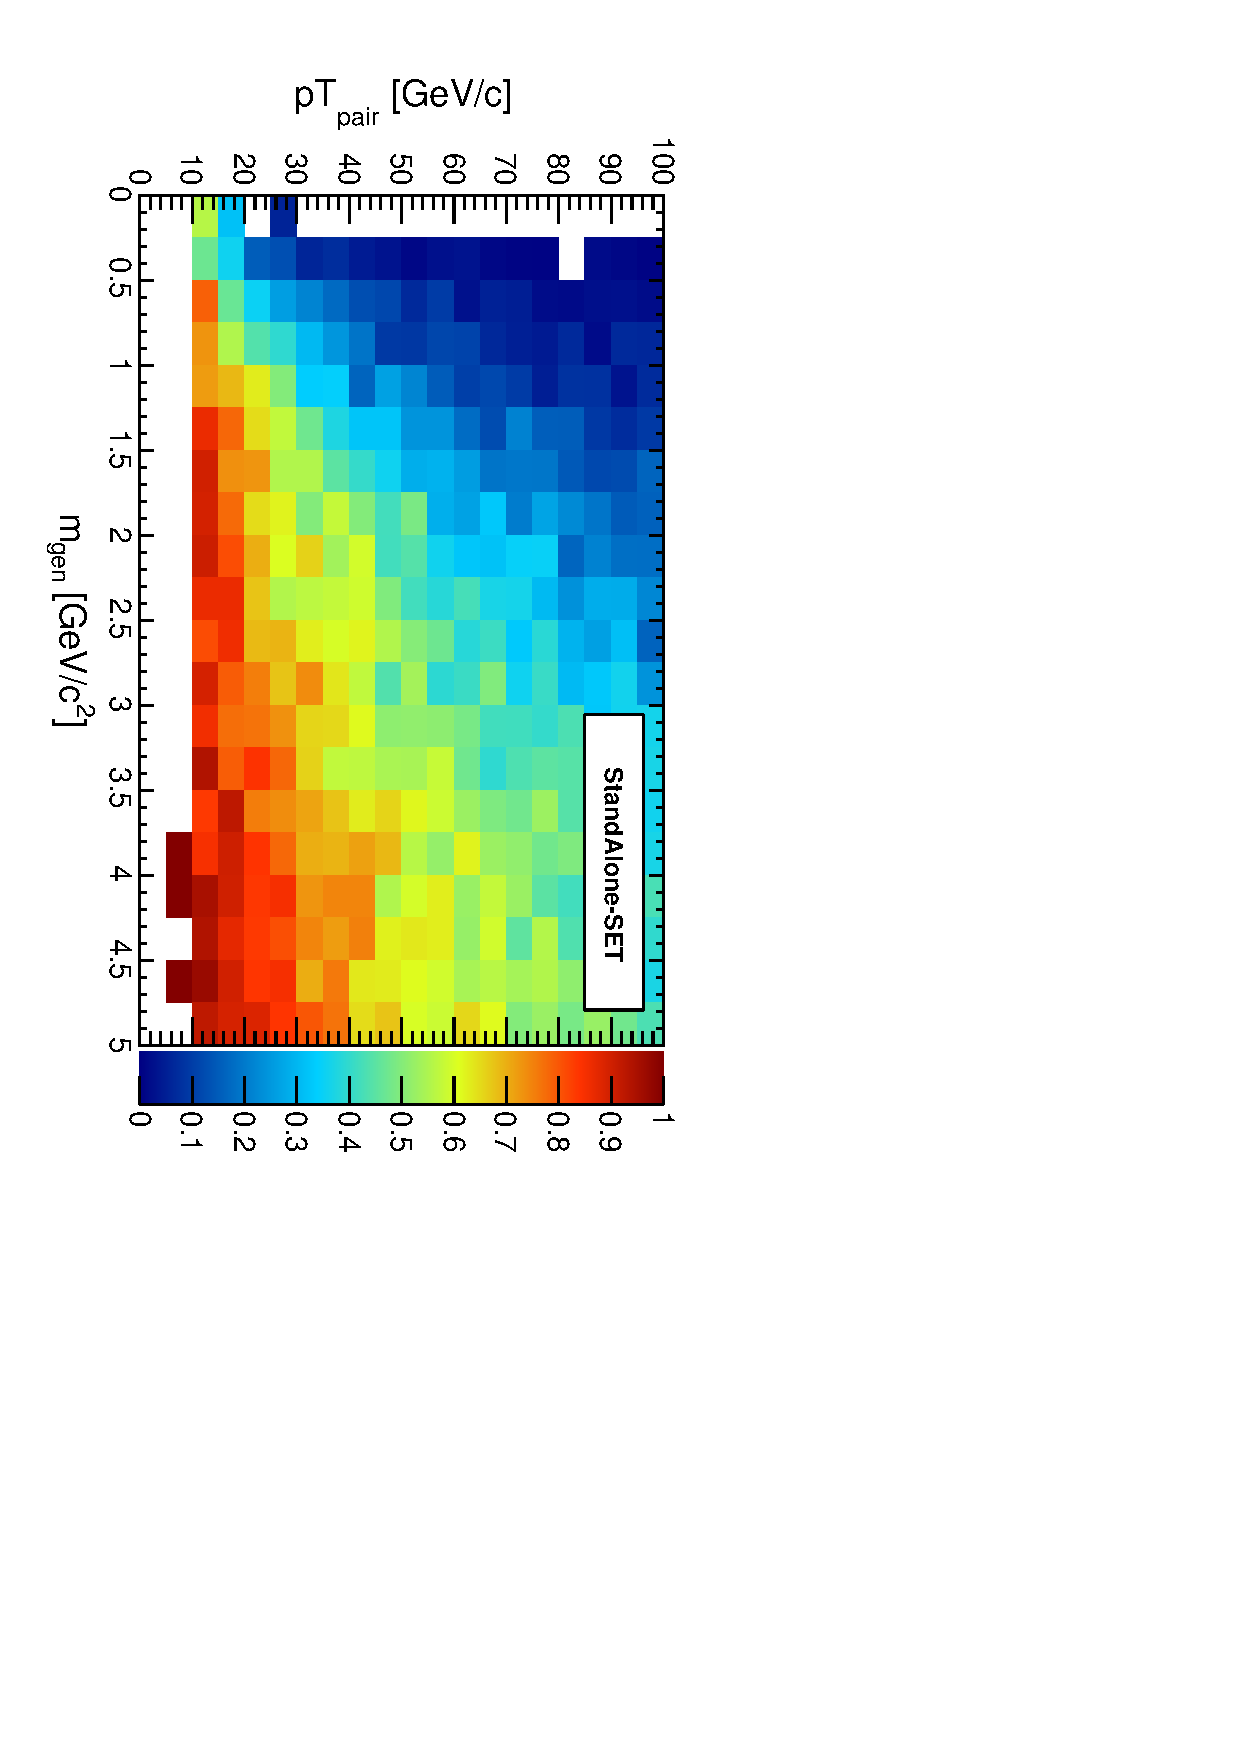
\includegraphics[height=0.5\linewidth, angle=90]{fig/acceptanceNoMCMatch_plot/pairptvsmass_StandAloneUpdatedSET.pdf}
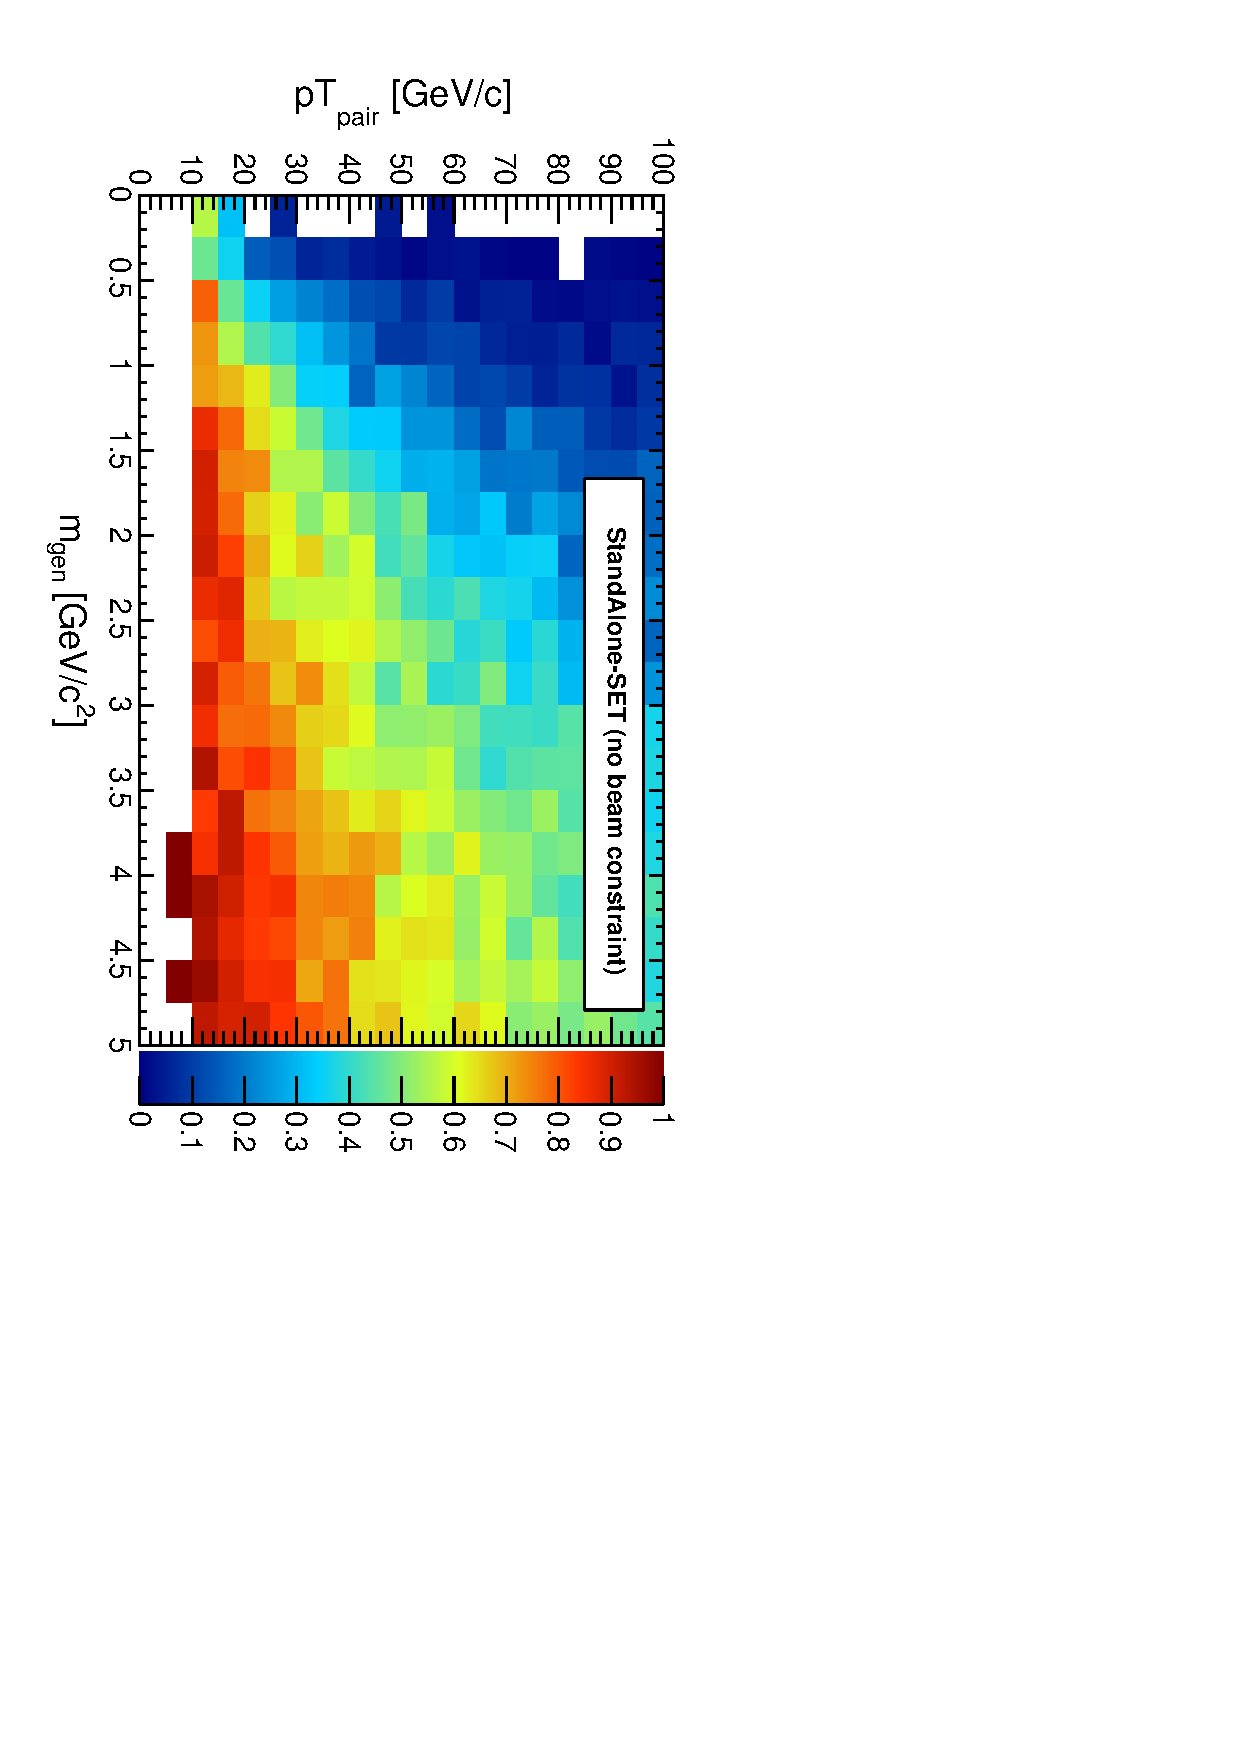
\includegraphics[height=0.5\linewidth, angle=90]{fig/acceptanceNoMCMatch_plot/pairptvsmass_StandAloneSET.pdf}

\caption{Same as Fig.~\ref{fig:pairptvsmass}, except that numerator
  only requires two reconstructed muons (no
  MC-matching). \label{fig:pairptvsmassNoMCMatch}}
\end{figure}

\begin{figure}
\begin{center}
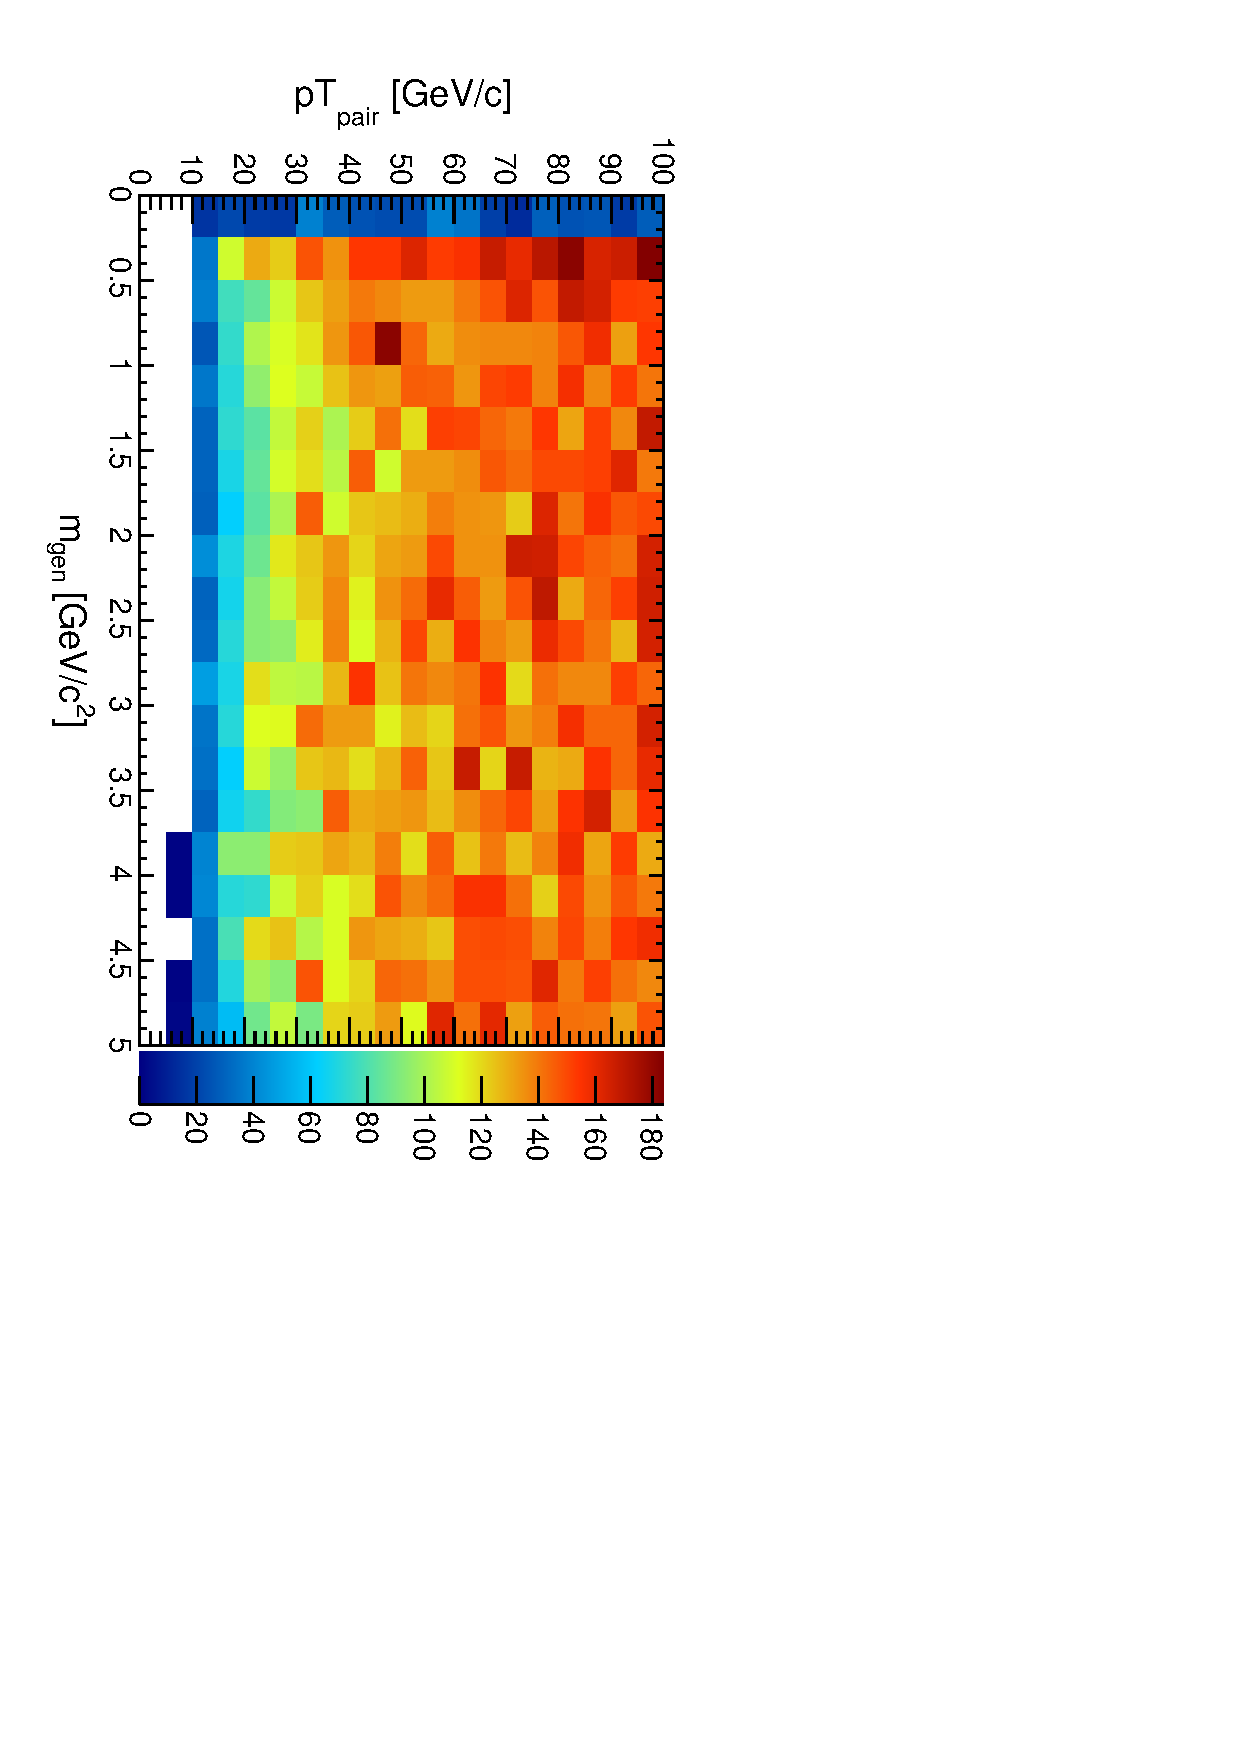
\includegraphics[height=0.5\linewidth, angle=90]{fig/acceptance_plot/pairptvsmass_TrackerMuons_denominator.pdf}
\end{center}
\caption{Denominator of plots in Figs.~\ref{fig:pairptvsmass} and \ref{fig:pairptvsmassNoMCMatch}.}
\end{figure}

\begin{figure}[p]
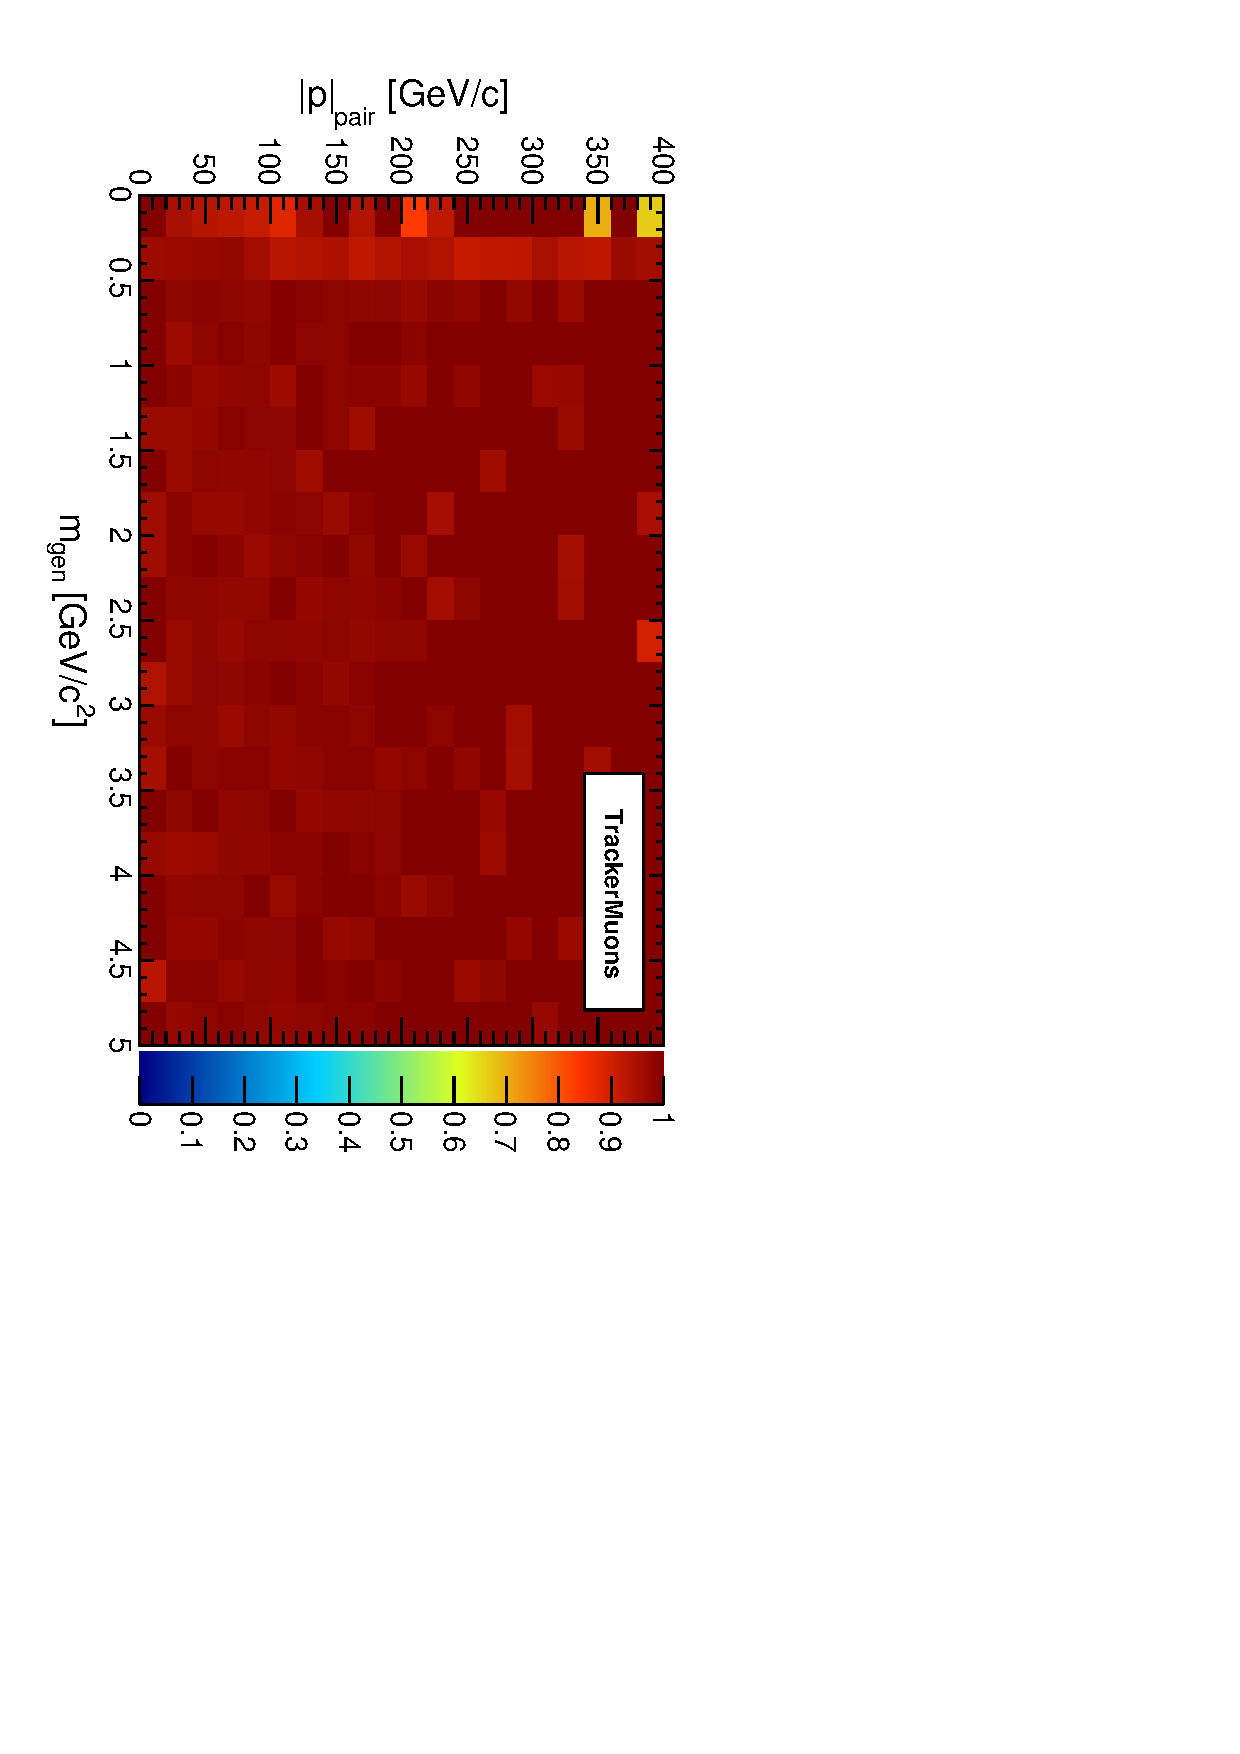
\includegraphics[height=0.5\linewidth, angle=90]{fig/acceptance_plot/pairpmagvsmass_TrackerMuons.pdf}
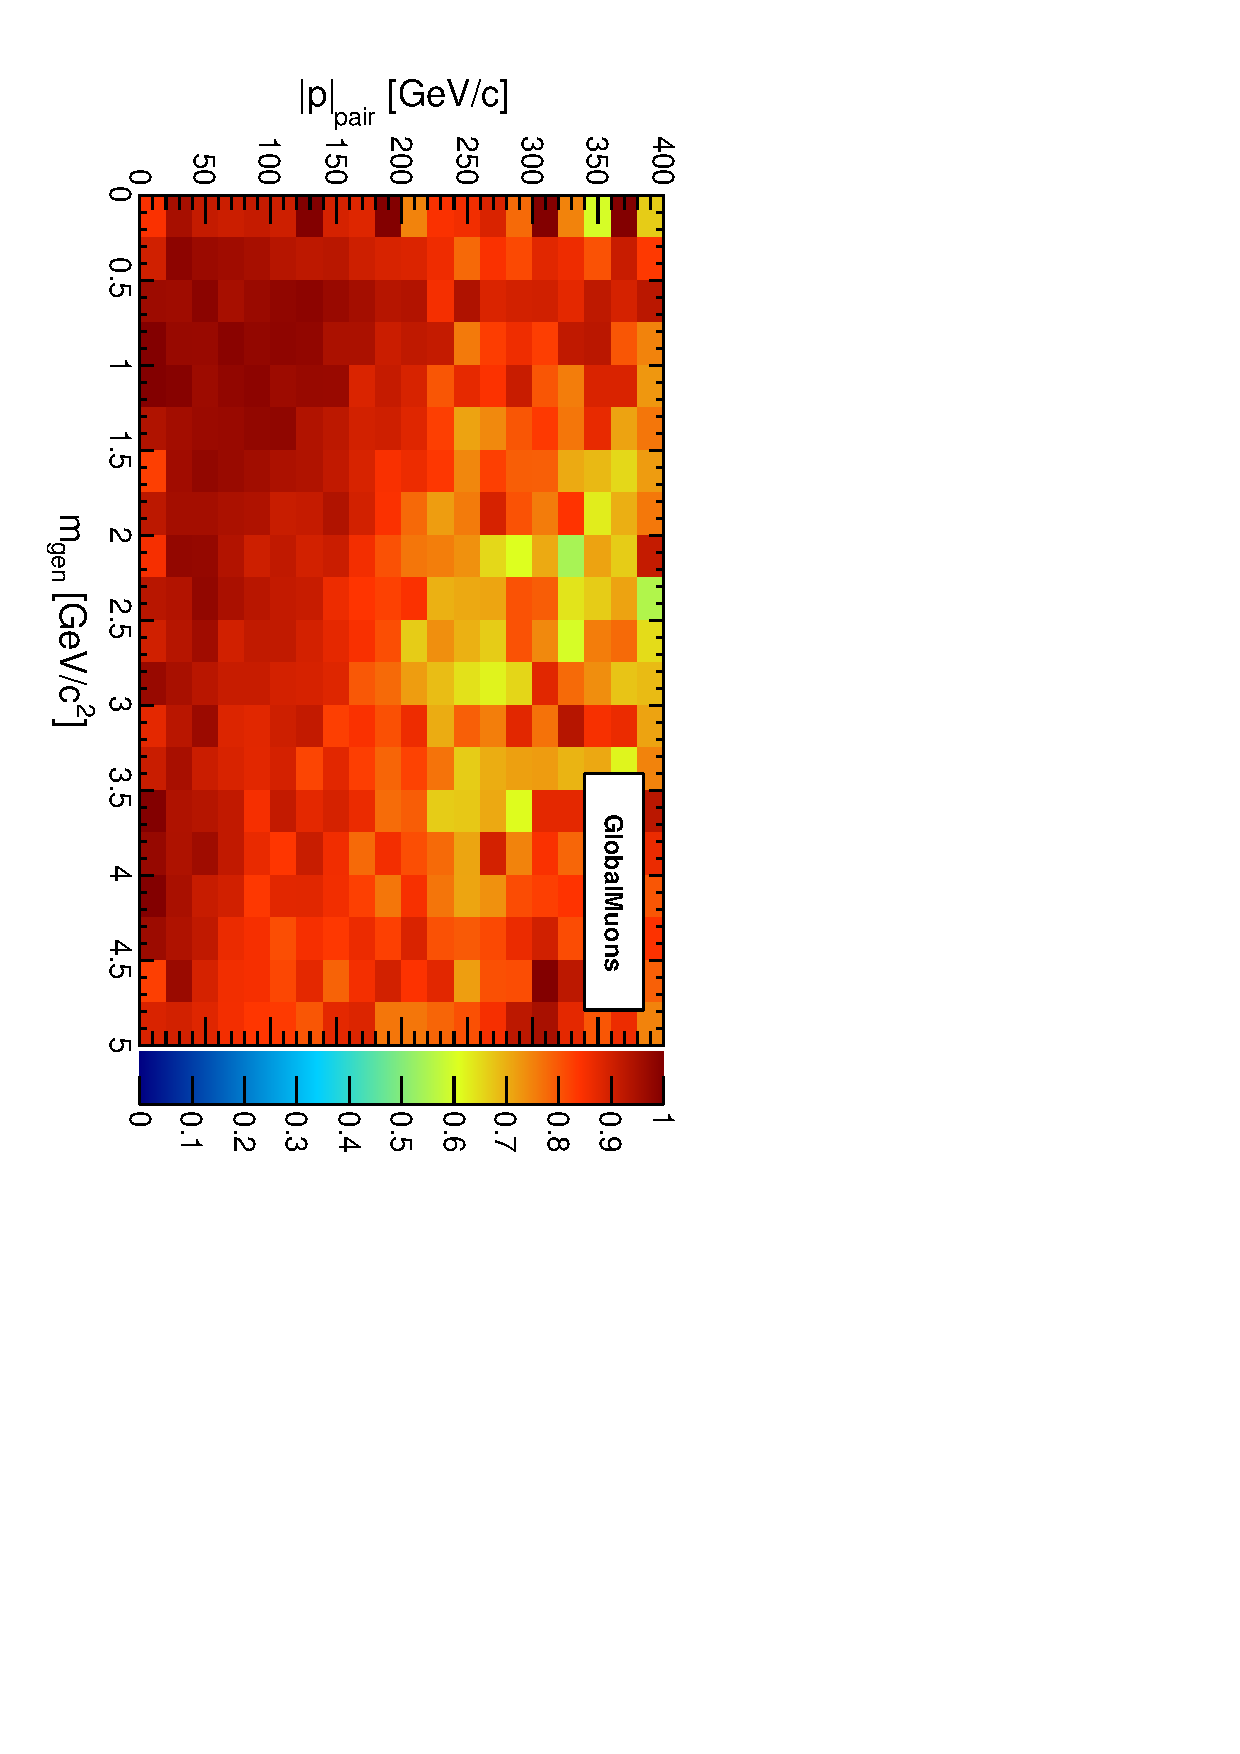
\includegraphics[height=0.5\linewidth, angle=90]{fig/acceptance_plot/pairpmagvsmass_GlobalMuons.pdf}

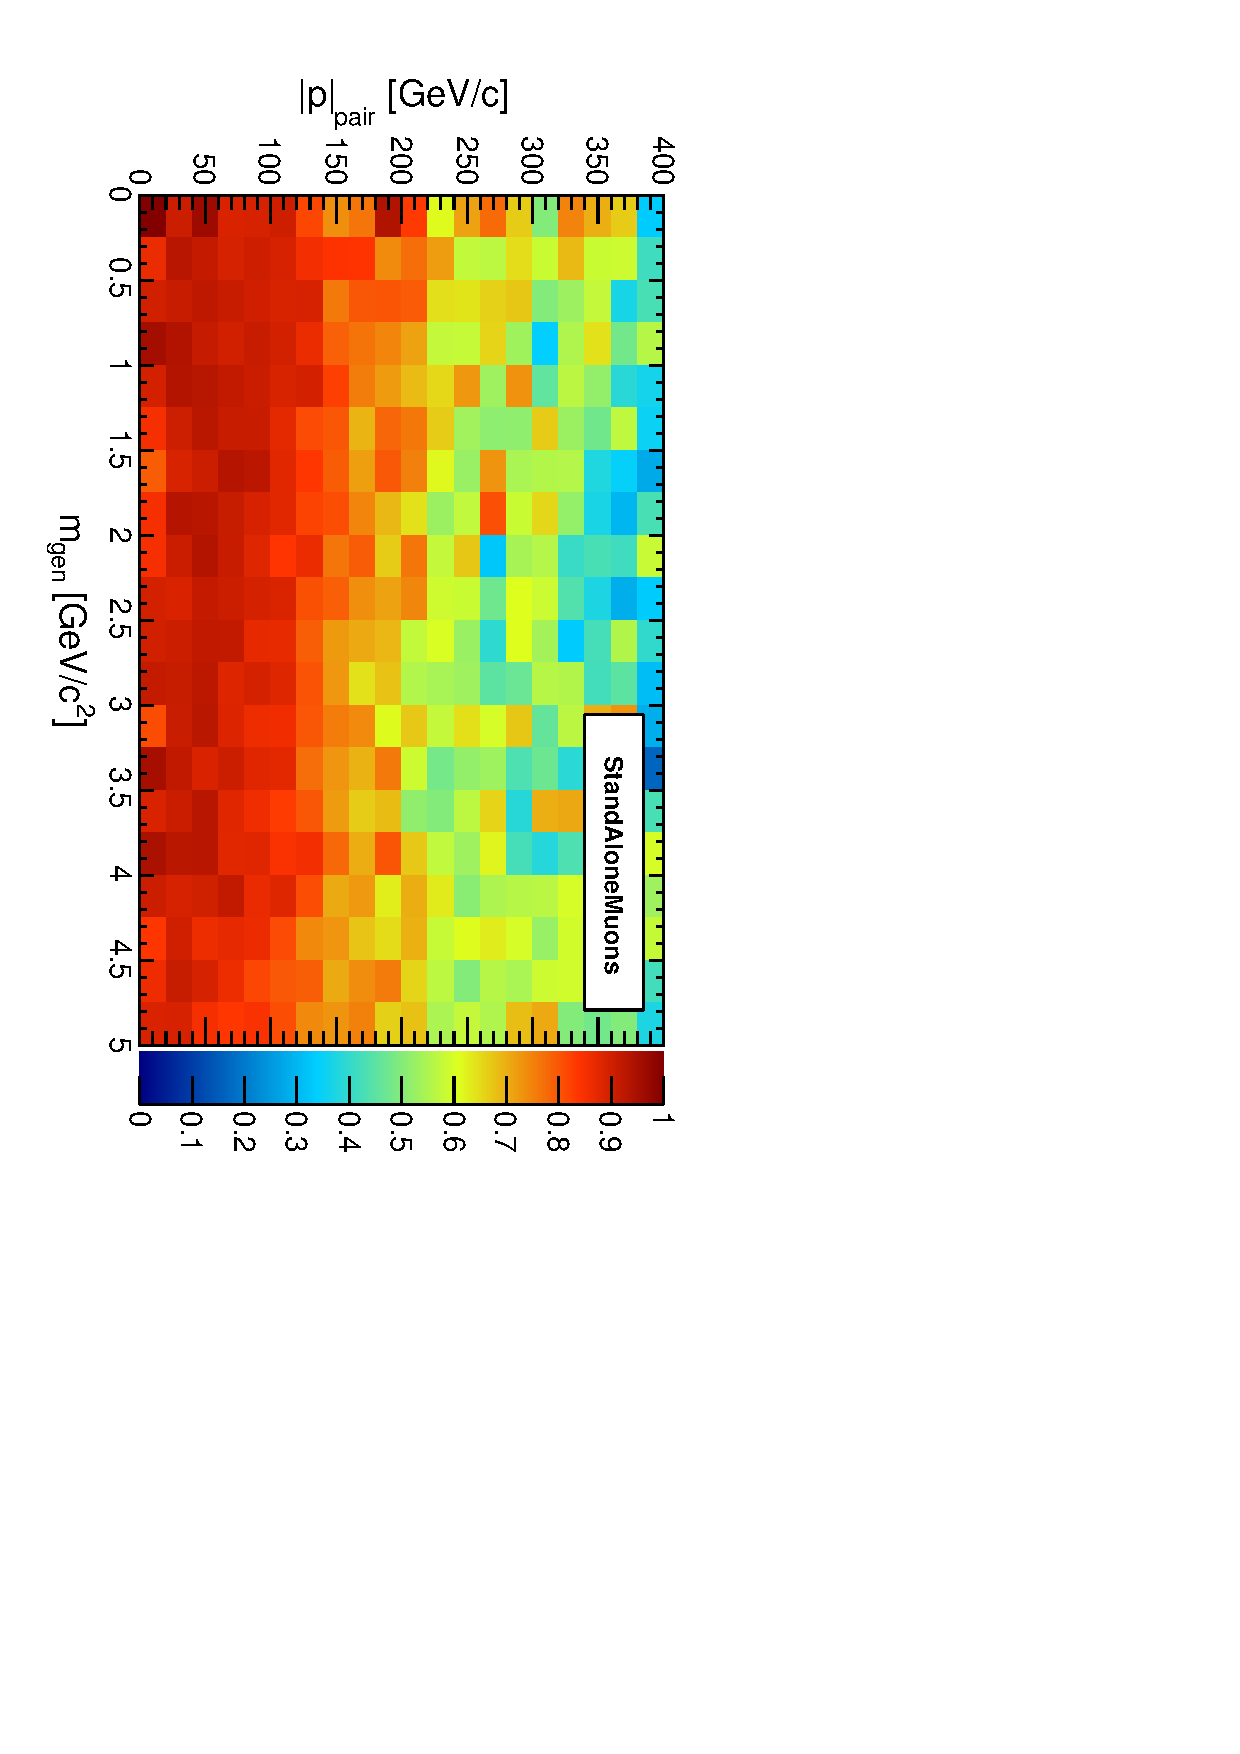
\includegraphics[height=0.5\linewidth, angle=90]{fig/acceptance_plot/pairpmagvsmass_StandAloneUpdatedDefault.pdf}
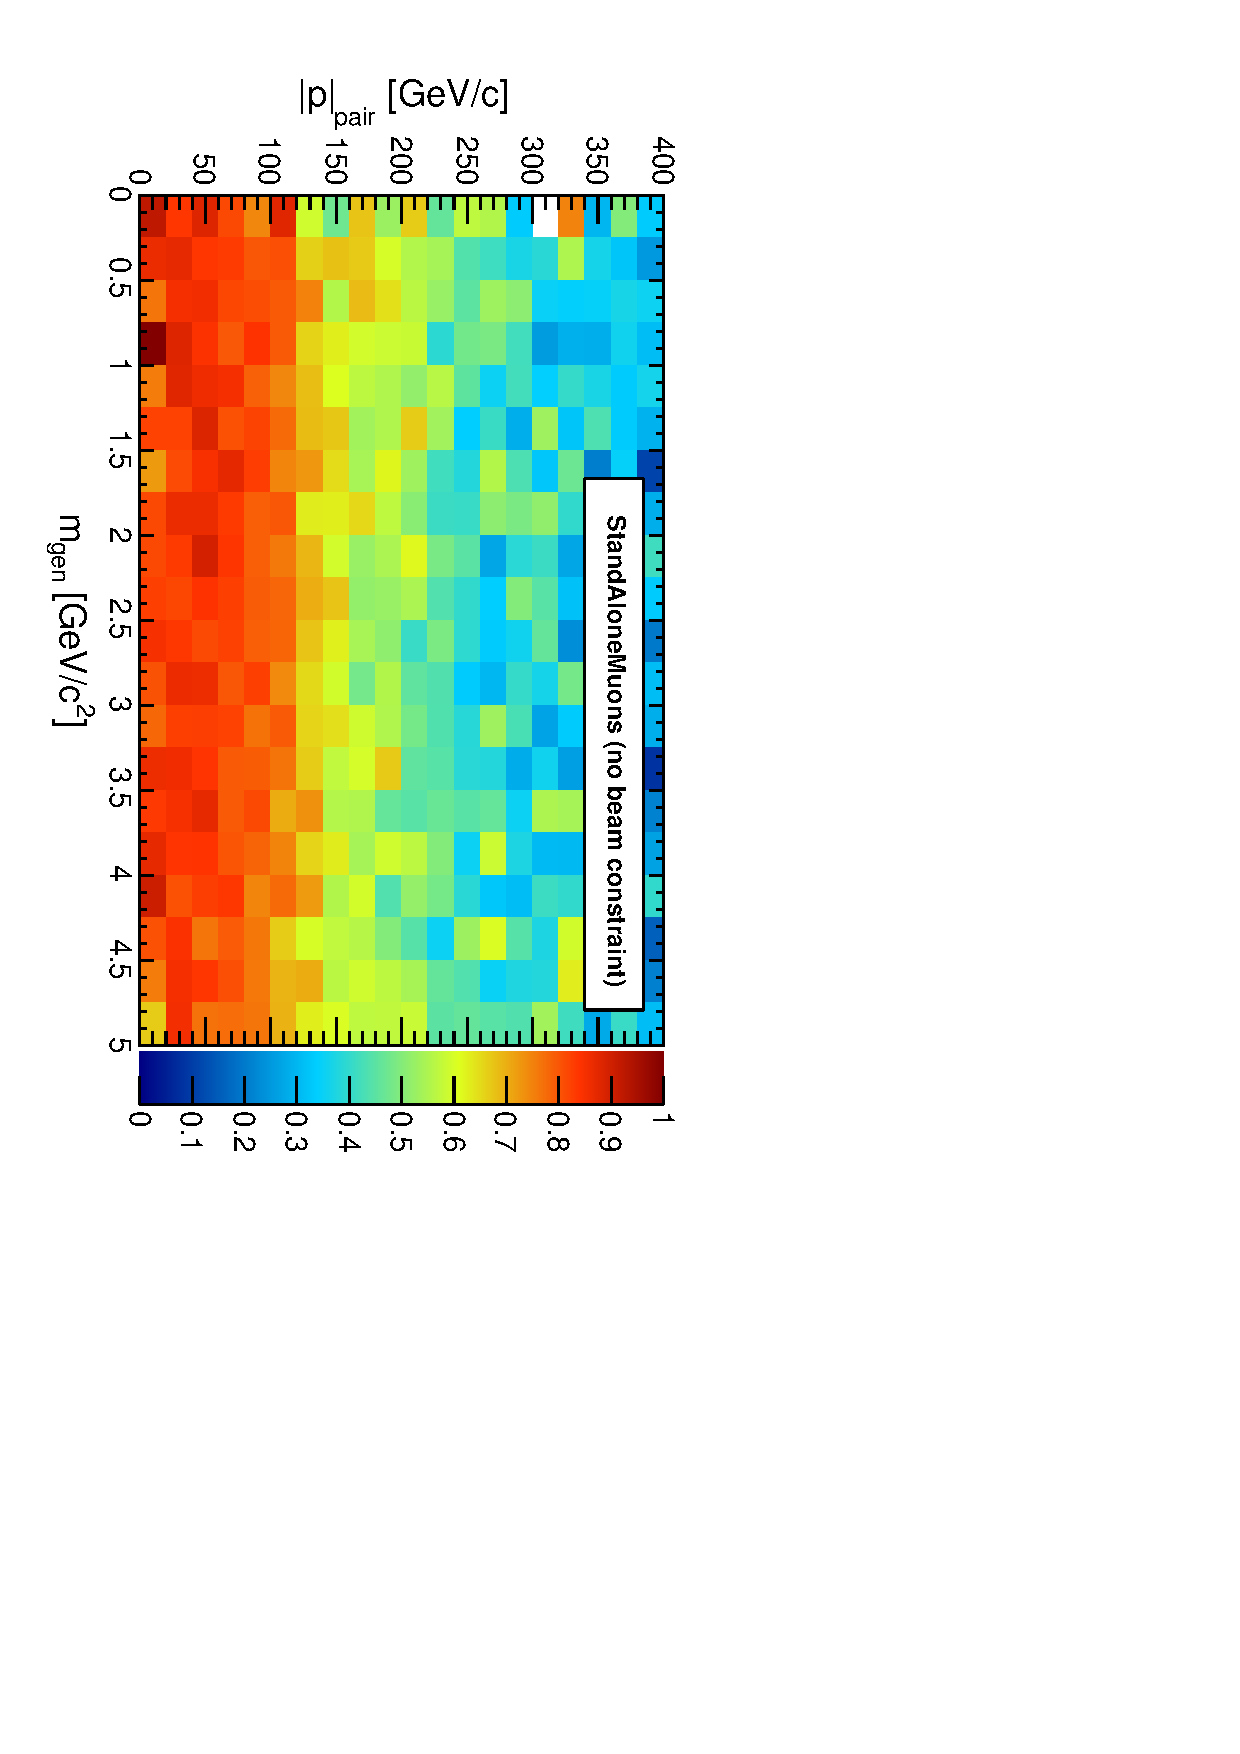
\includegraphics[height=0.5\linewidth, angle=90]{fig/acceptance_plot/pairpmagvsmass_StandAloneDefault.pdf}

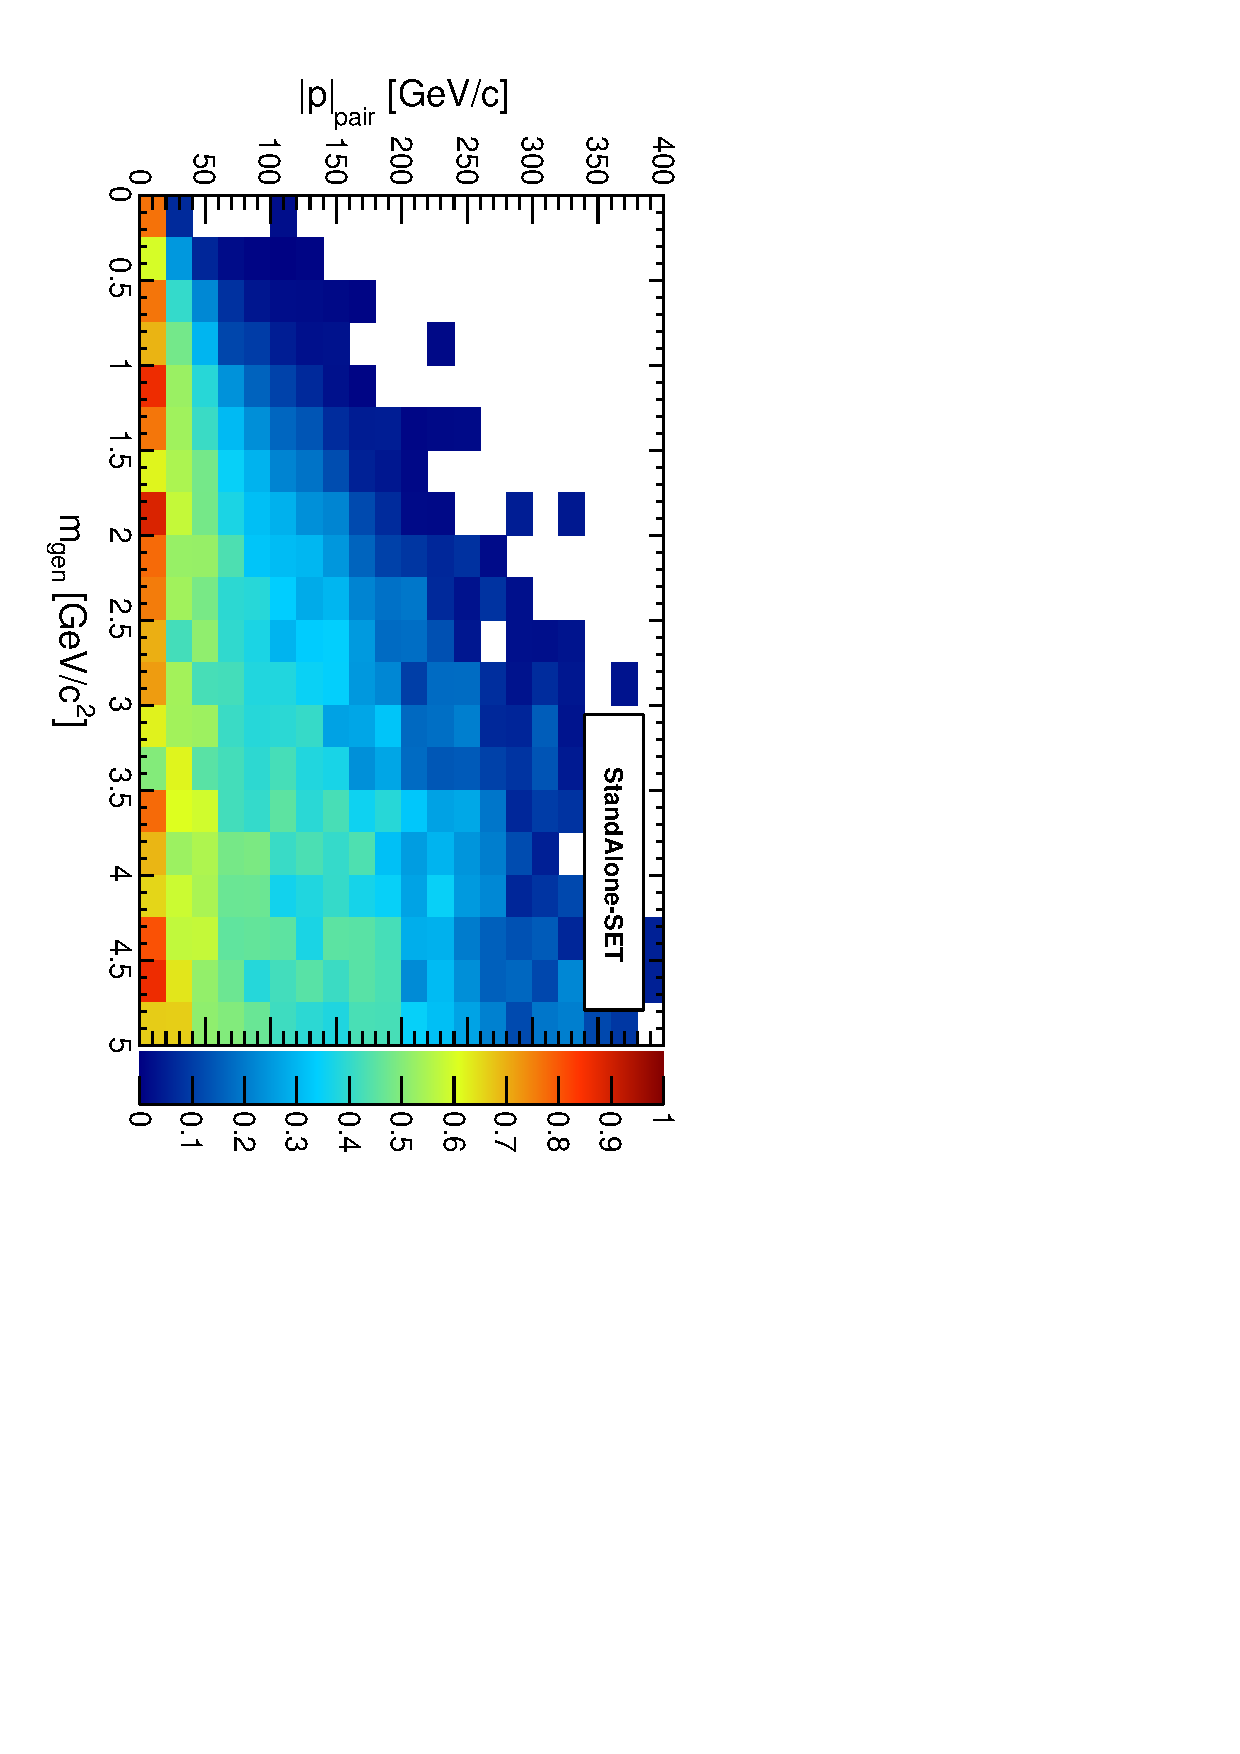
\includegraphics[height=0.5\linewidth, angle=90]{fig/acceptance_plot/pairpmagvsmass_StandAloneUpdatedSET.pdf}
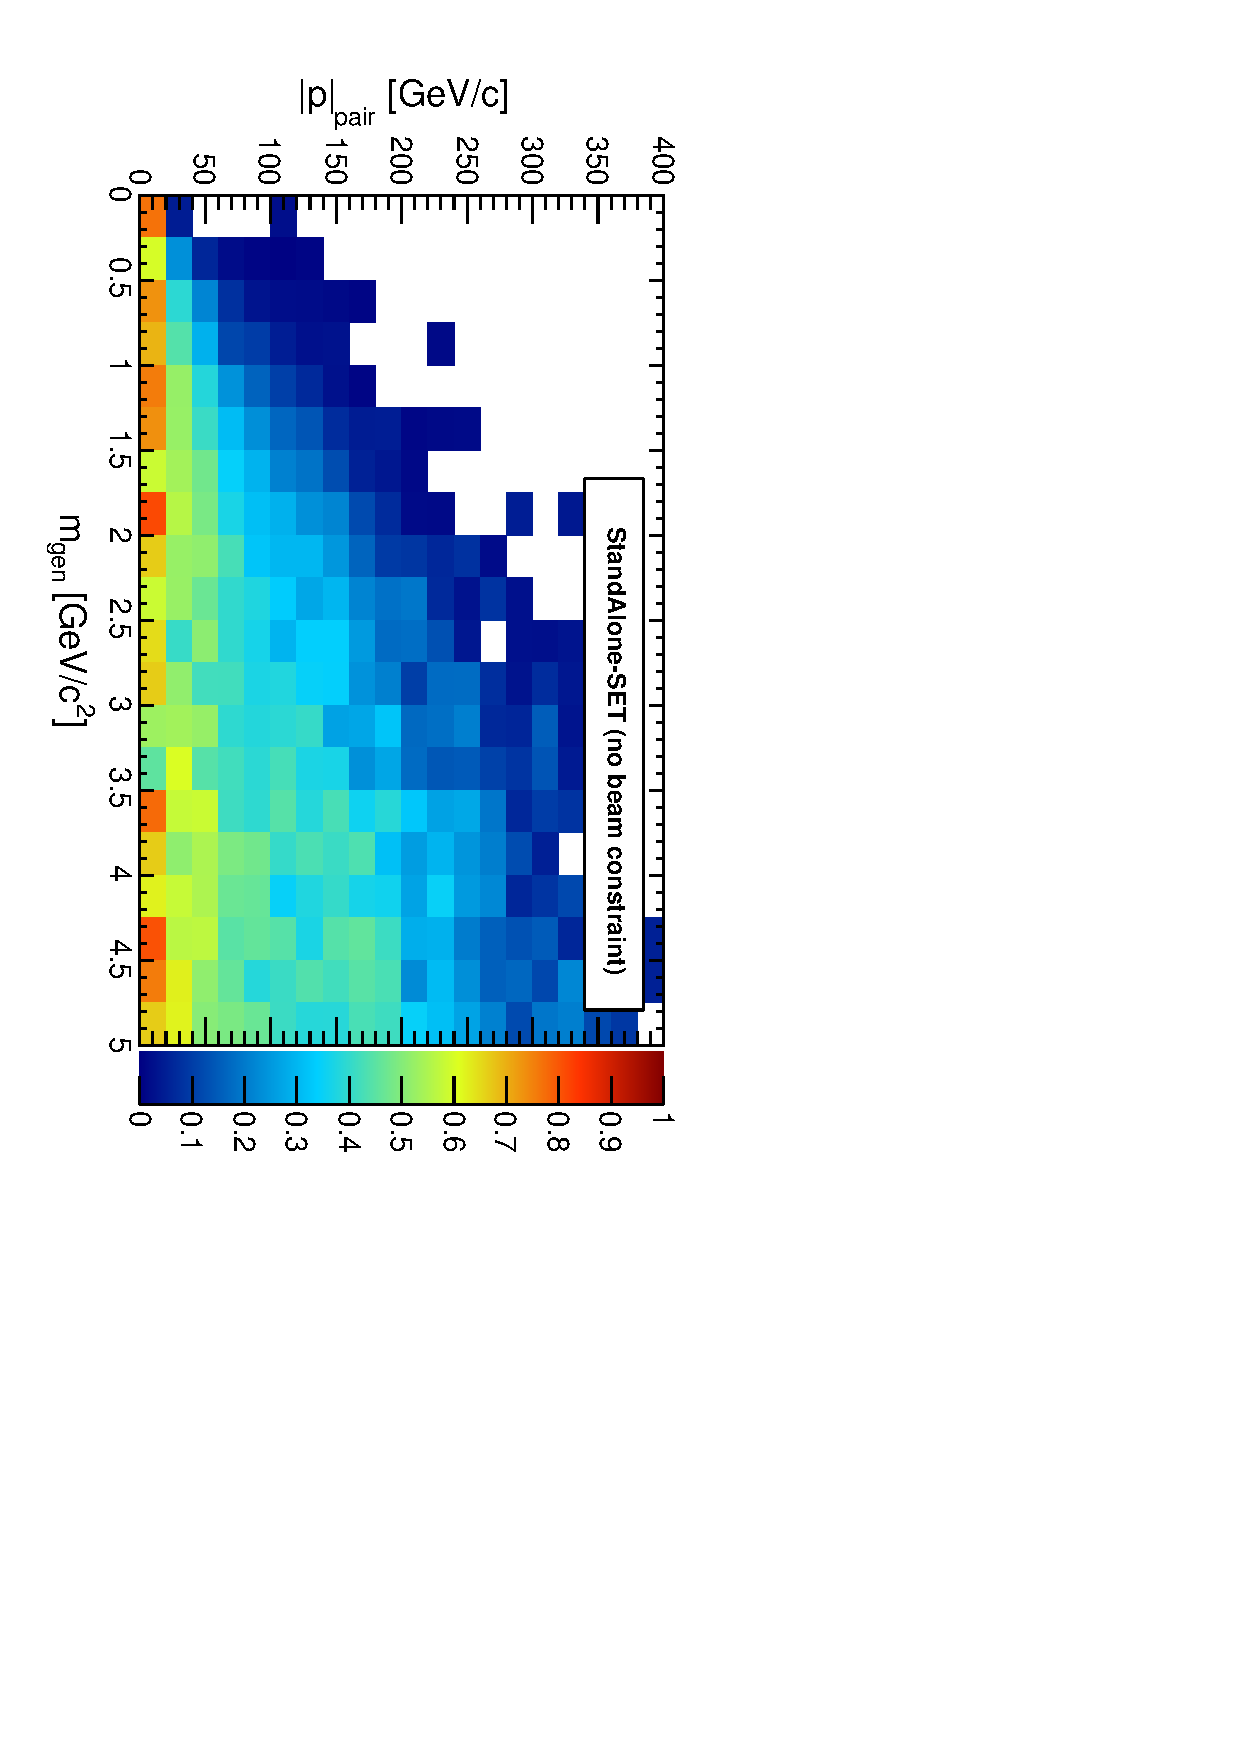
\includegraphics[height=0.5\linewidth, angle=90]{fig/acceptance_plot/pairpmagvsmass_StandAloneSET.pdf}

\caption{Efficiency as a function of physics-relevant variables:
  $|\vec{p}|$ and invariant mass of the $\mu^+$-$\mu^-$ pair.
  Denominator: generated events with $pT_2 > 5$~GeV/$c$ and $|\eta_1|
  < 2.4$; numerator: reconstructed and MC-matched $\mu^+$ and $\mu^-$.
  \fixme{Vadim recommends higher range in $|\vec{p}|$, say
    400~GeV/$c$.} \label{fig:pairpmagvsmass}}
\end{figure}

\begin{figure}[p]
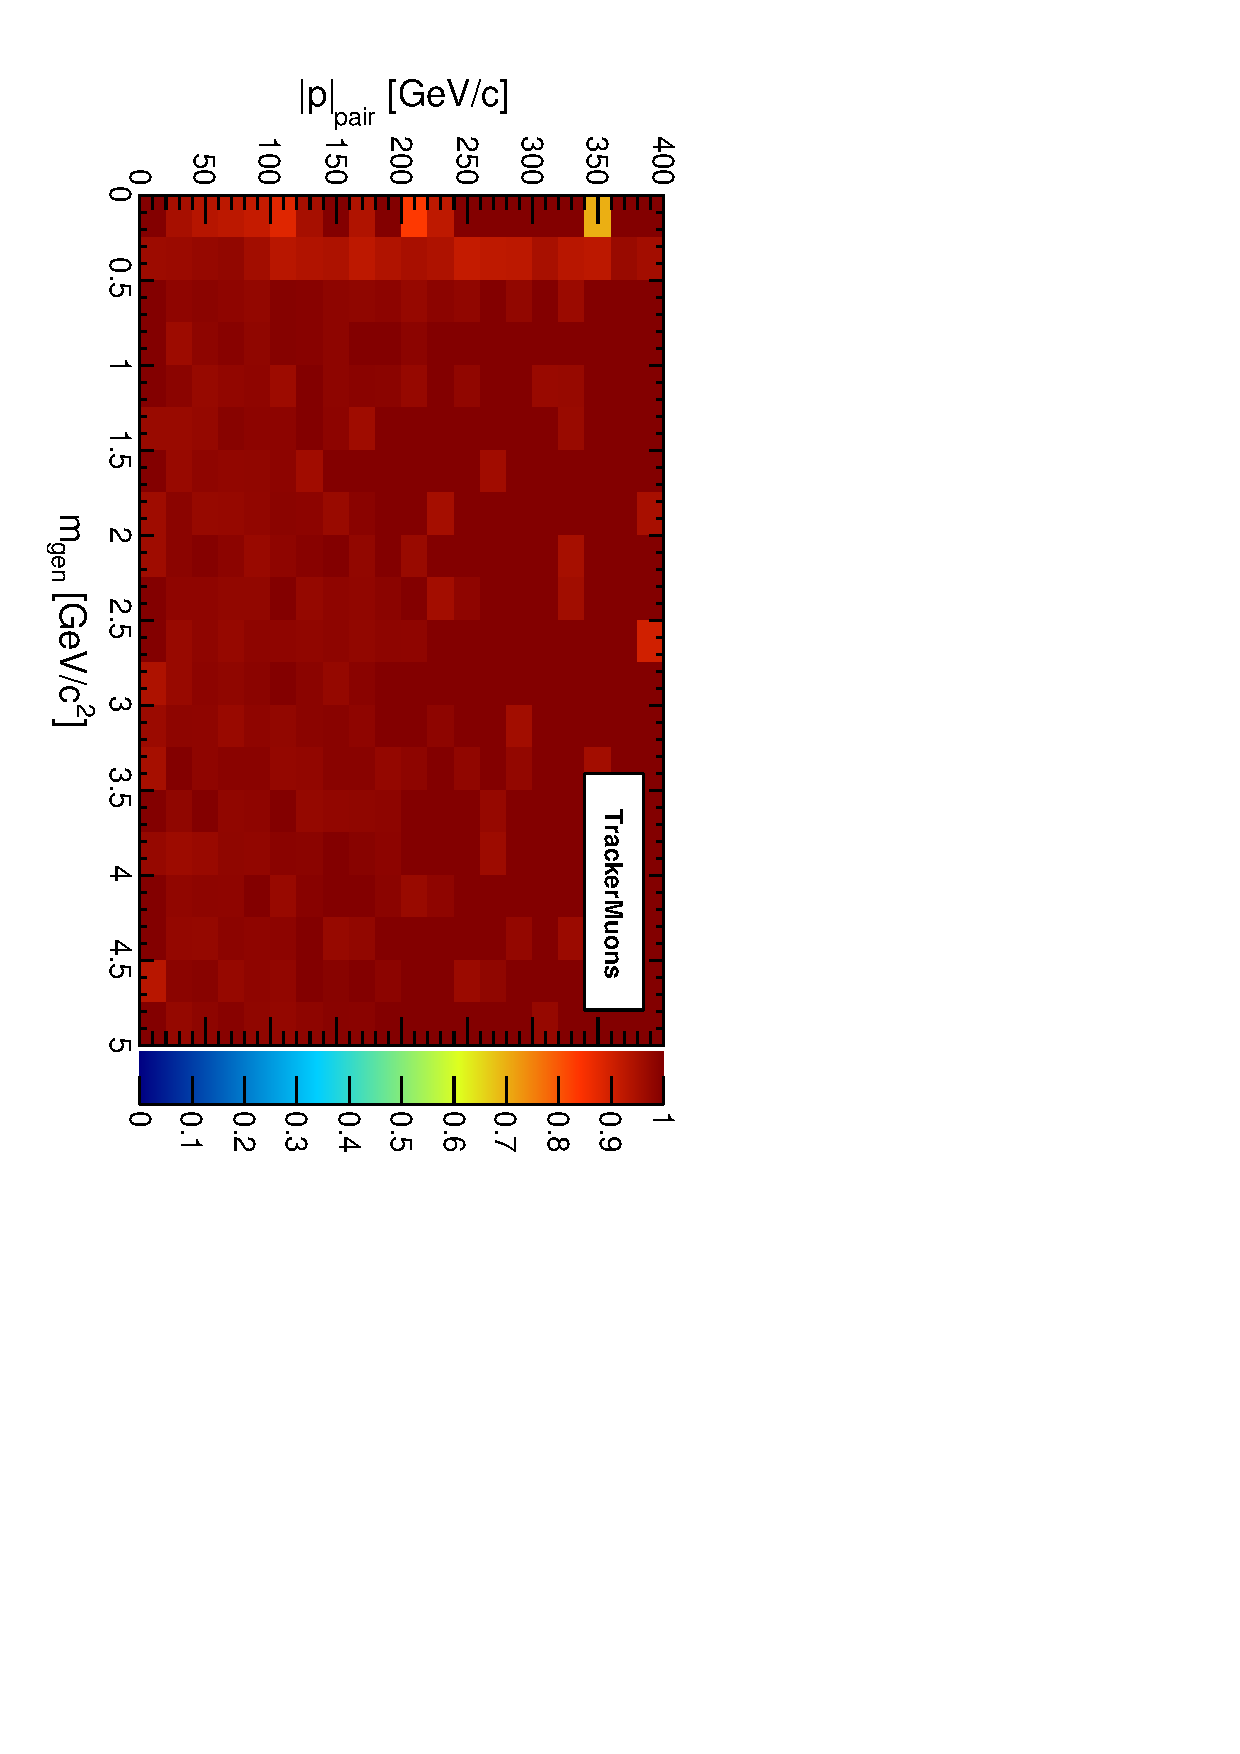
\includegraphics[height=0.5\linewidth, angle=90]{fig/acceptanceNoMCMatch_plot/pairpmagvsmass_TrackerMuons.pdf}
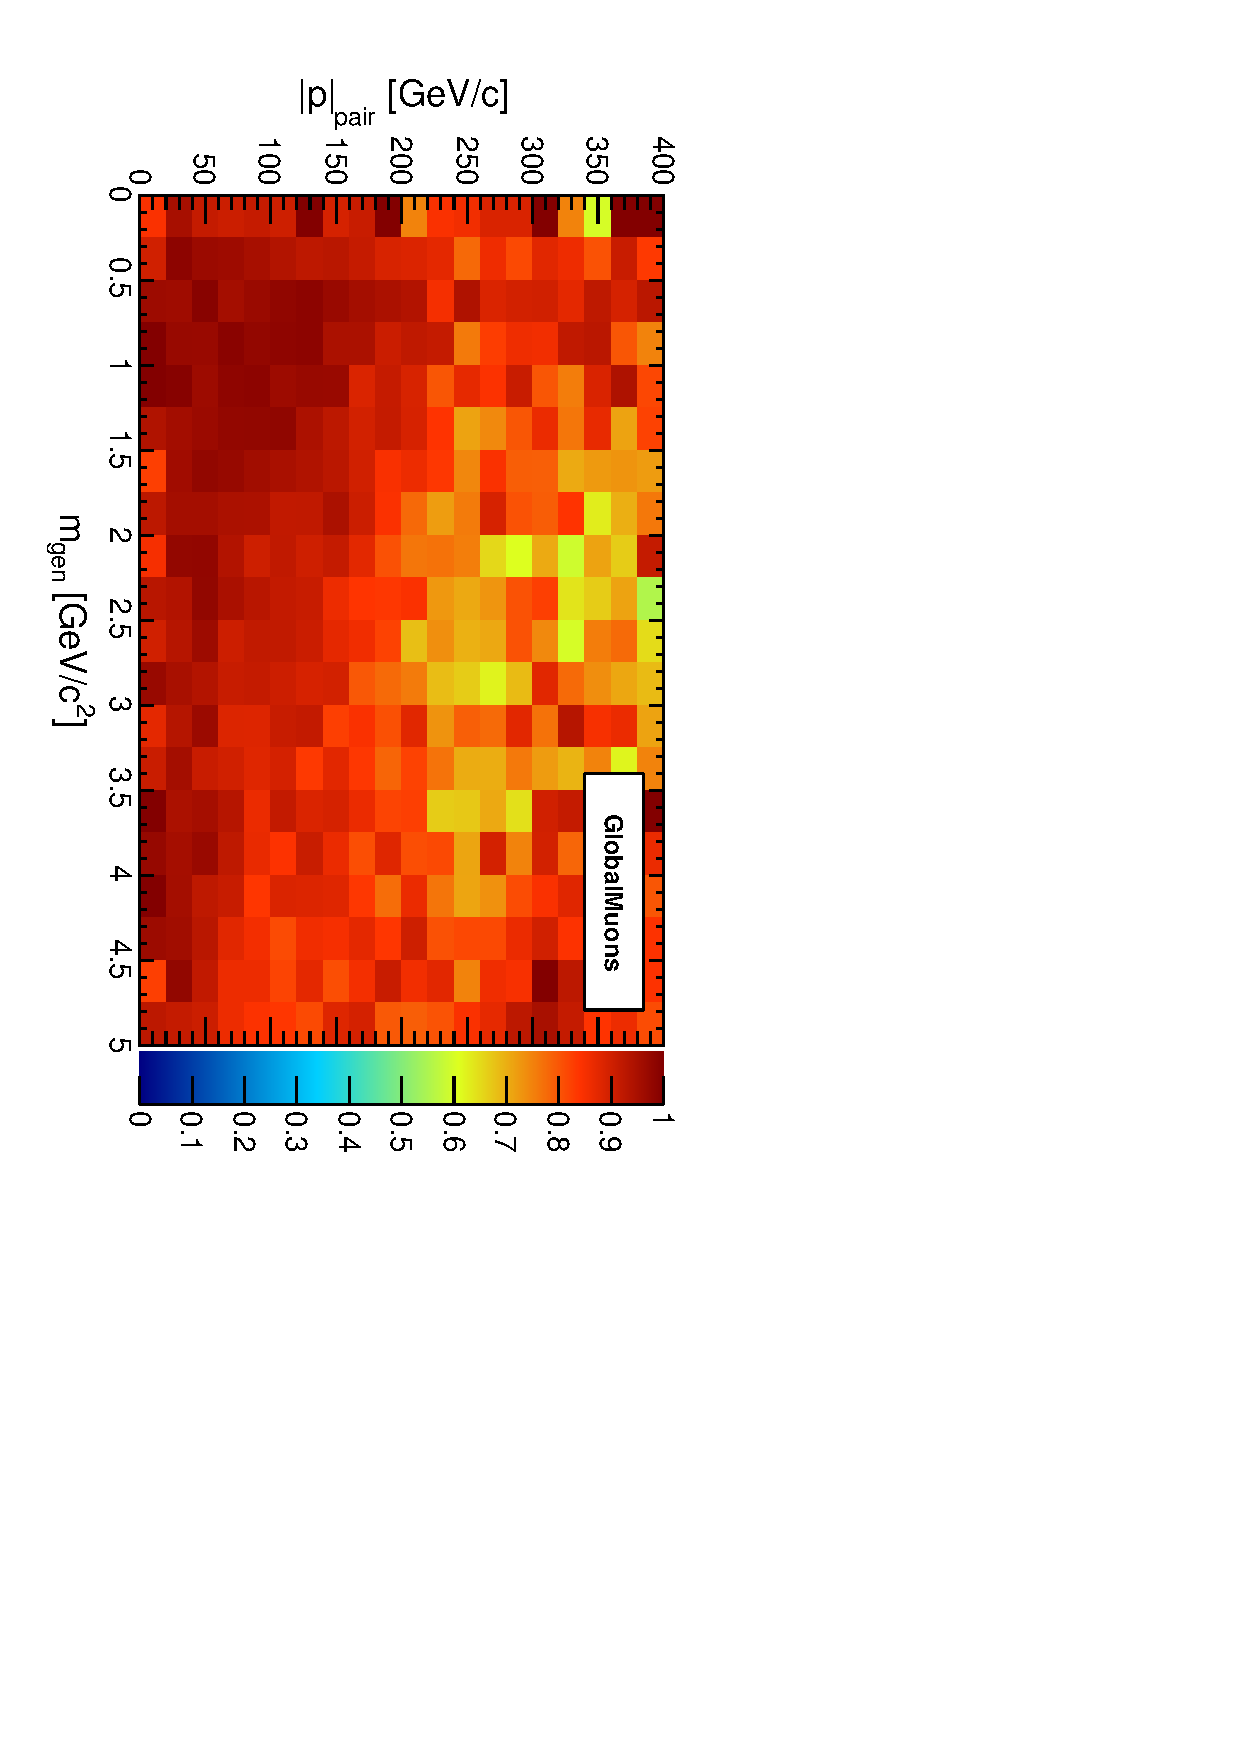
\includegraphics[height=0.5\linewidth, angle=90]{fig/acceptanceNoMCMatch_plot/pairpmagvsmass_GlobalMuons.pdf}

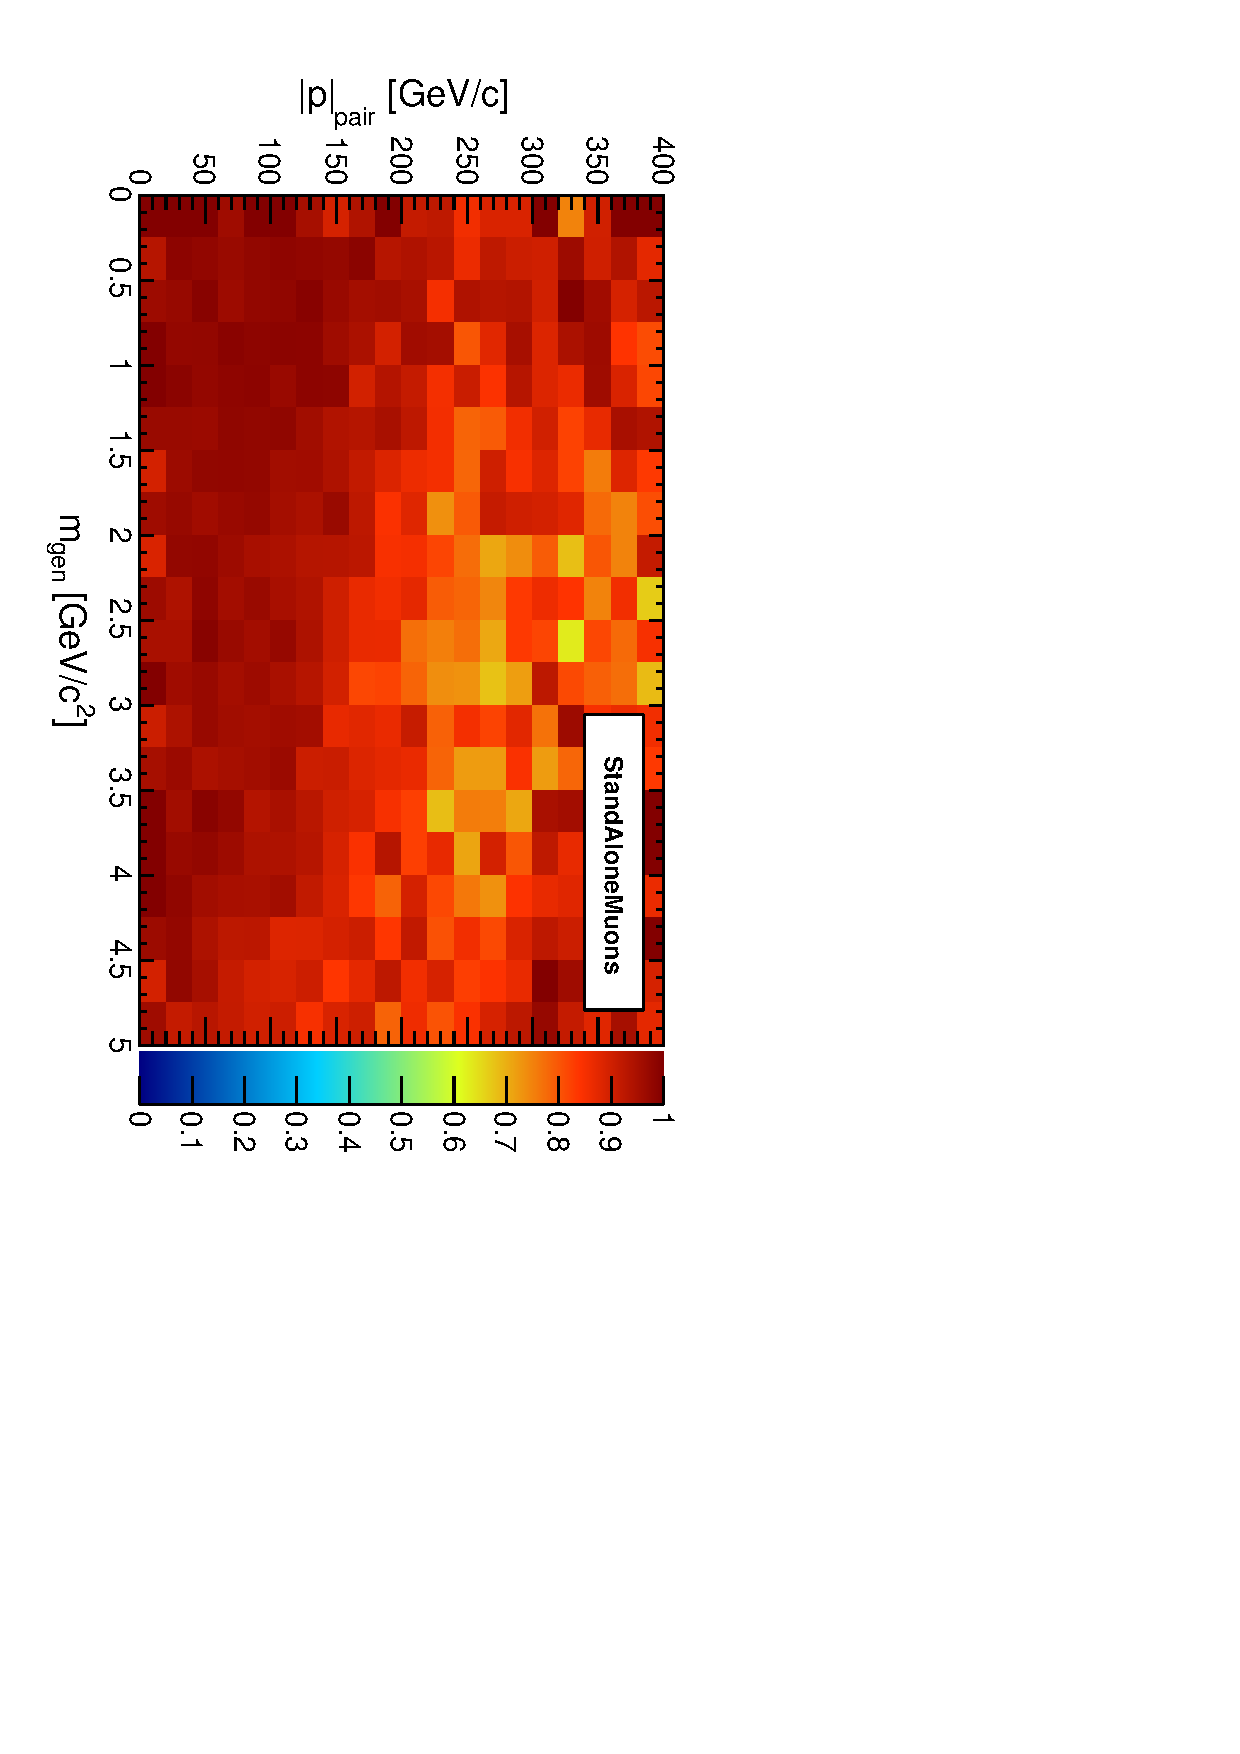
\includegraphics[height=0.5\linewidth, angle=90]{fig/acceptanceNoMCMatch_plot/pairpmagvsmass_StandAloneUpdatedDefault.pdf}
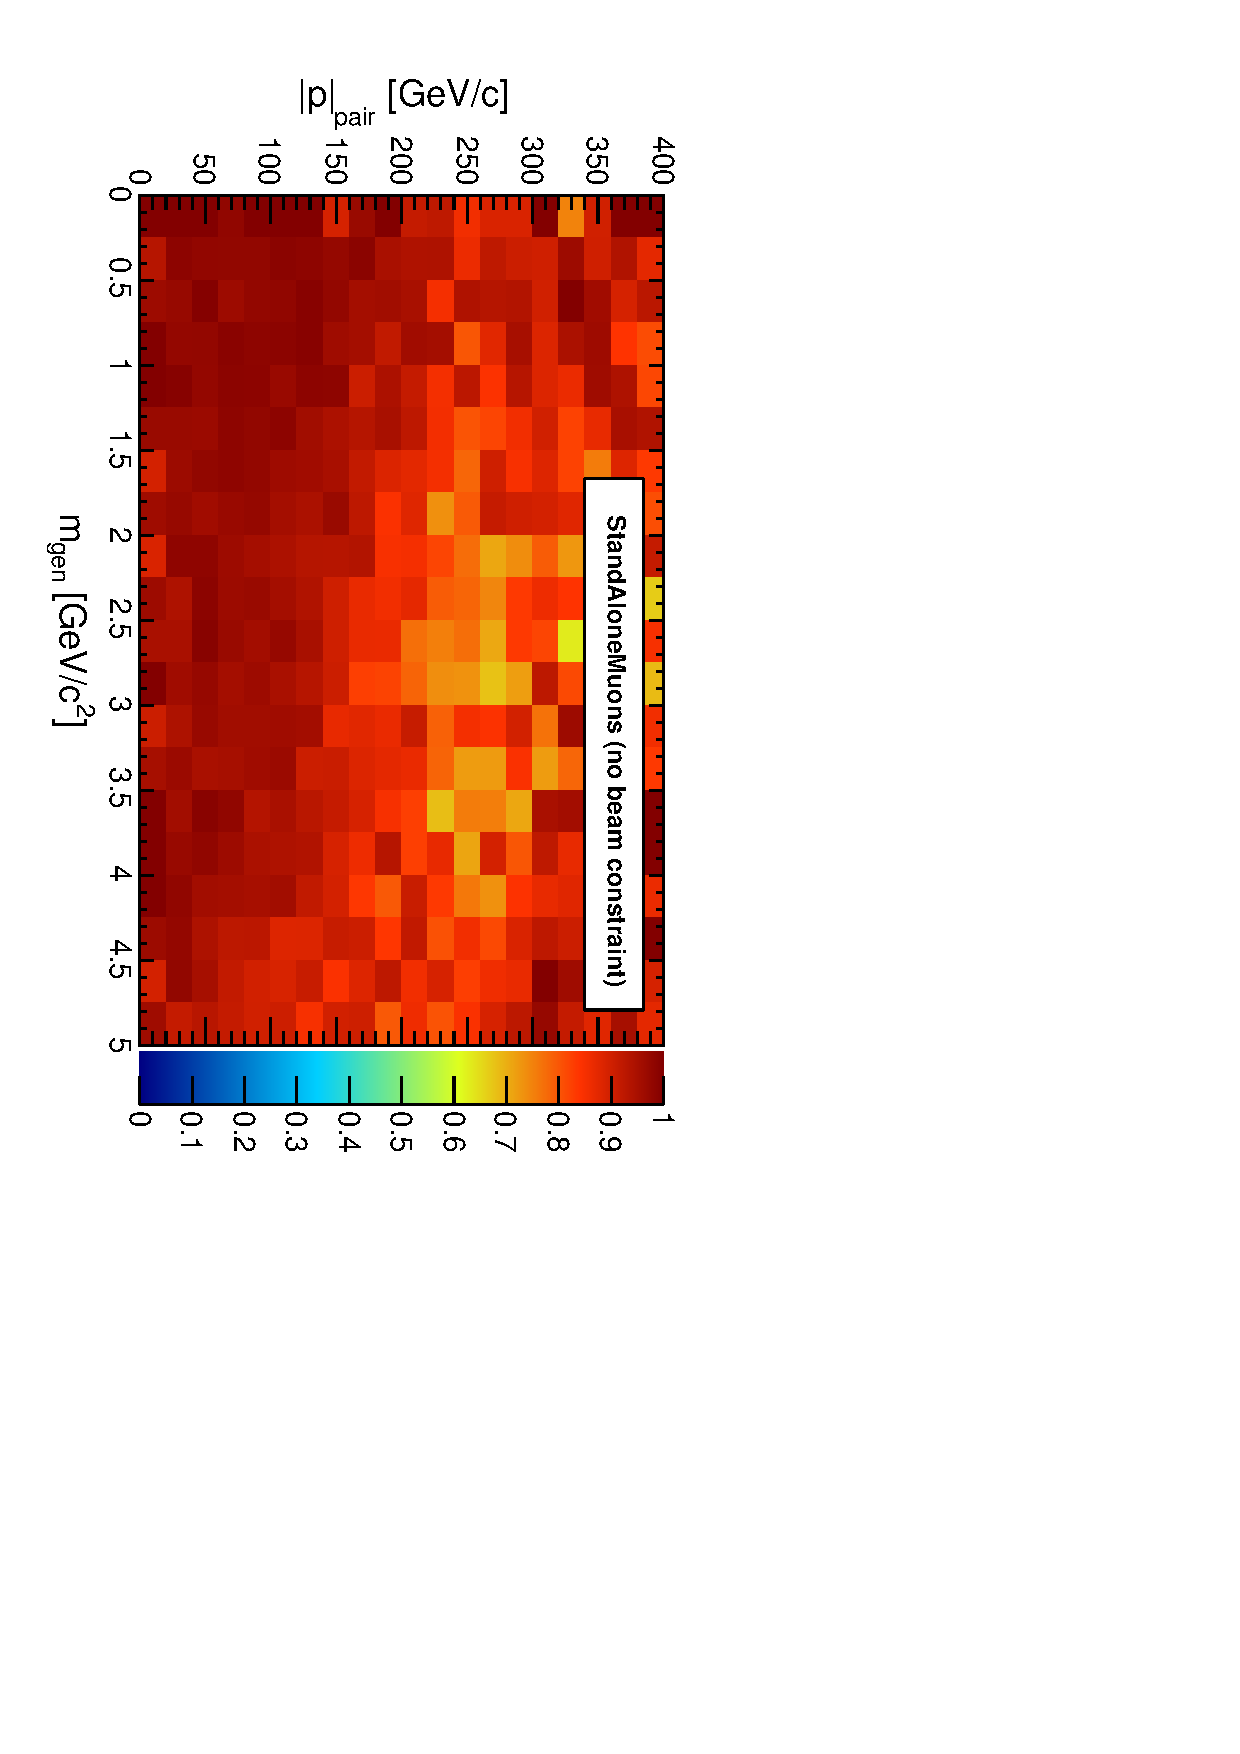
\includegraphics[height=0.5\linewidth, angle=90]{fig/acceptanceNoMCMatch_plot/pairpmagvsmass_StandAloneDefault.pdf}

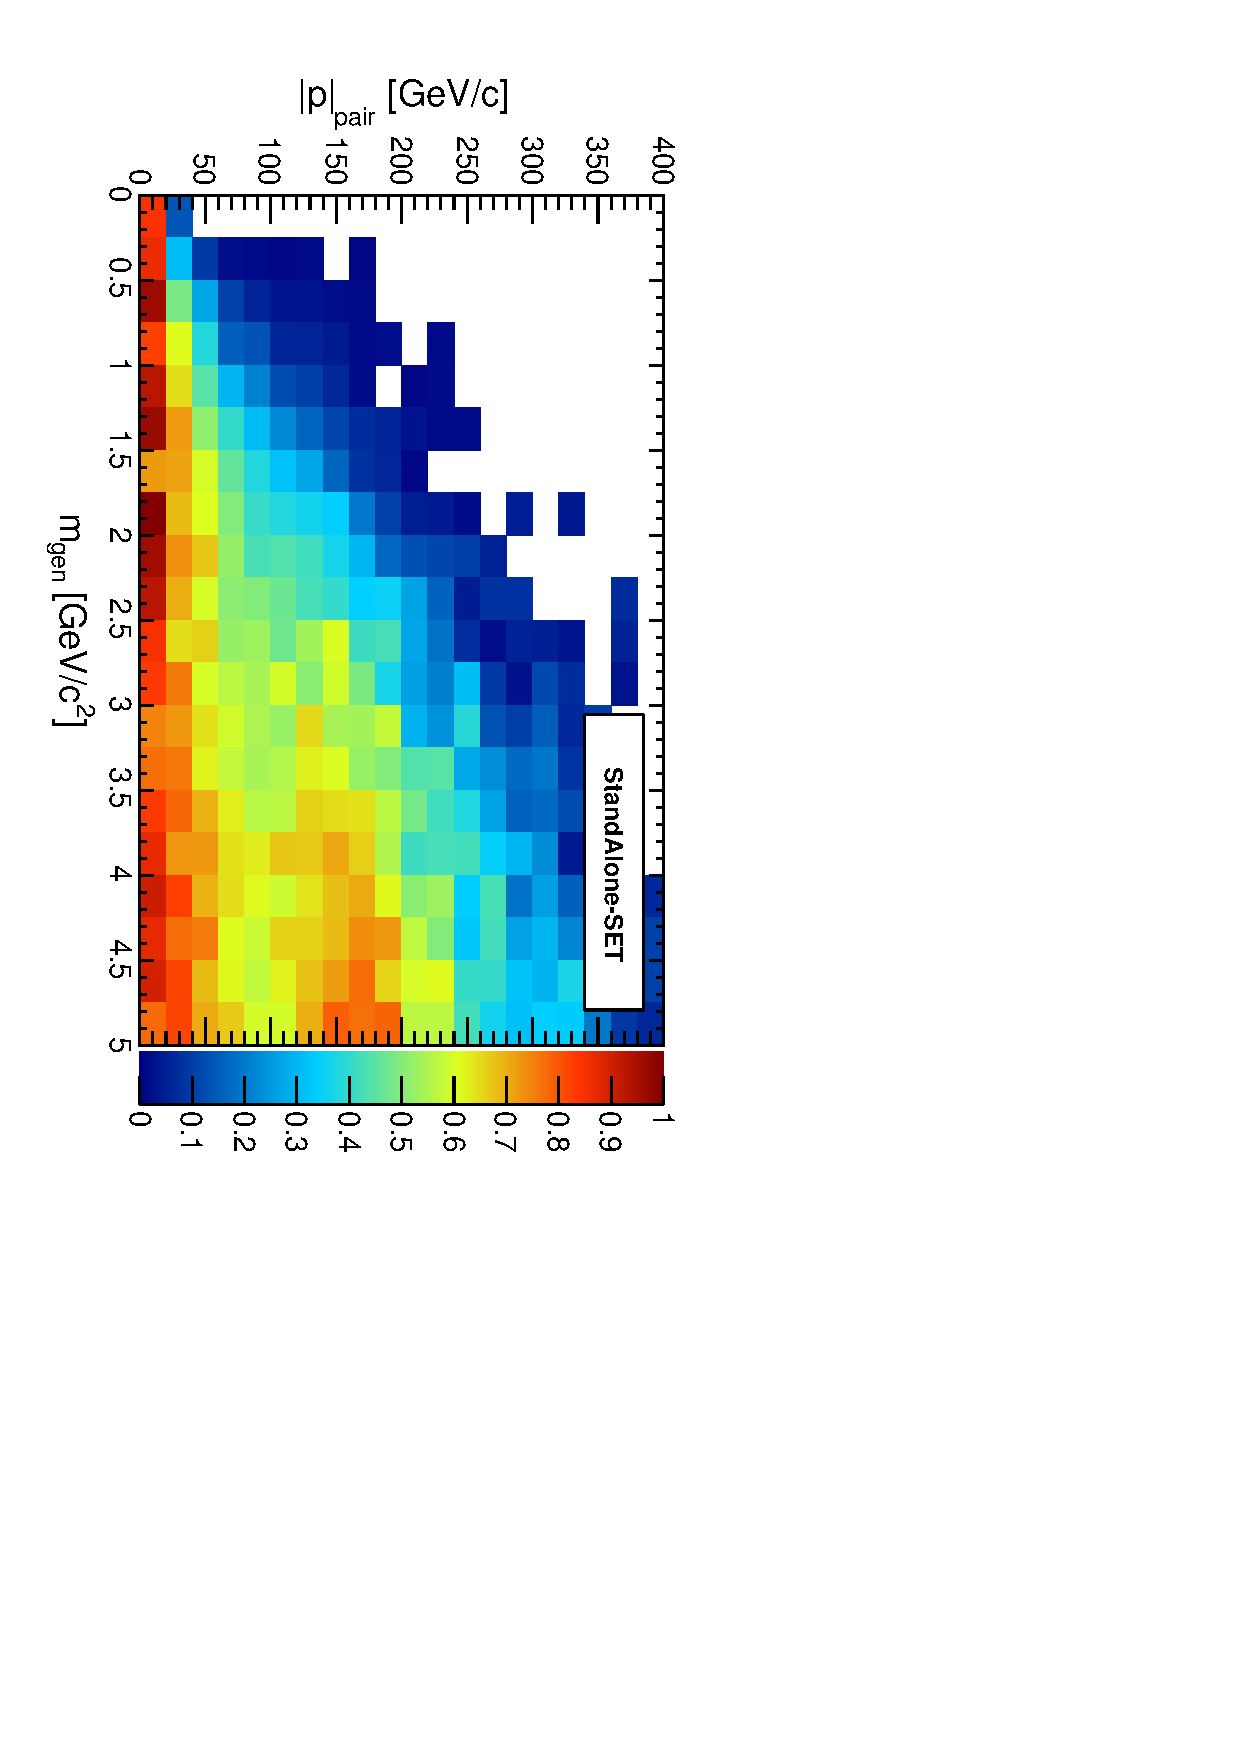
\includegraphics[height=0.5\linewidth, angle=90]{fig/acceptanceNoMCMatch_plot/pairpmagvsmass_StandAloneUpdatedSET.pdf}
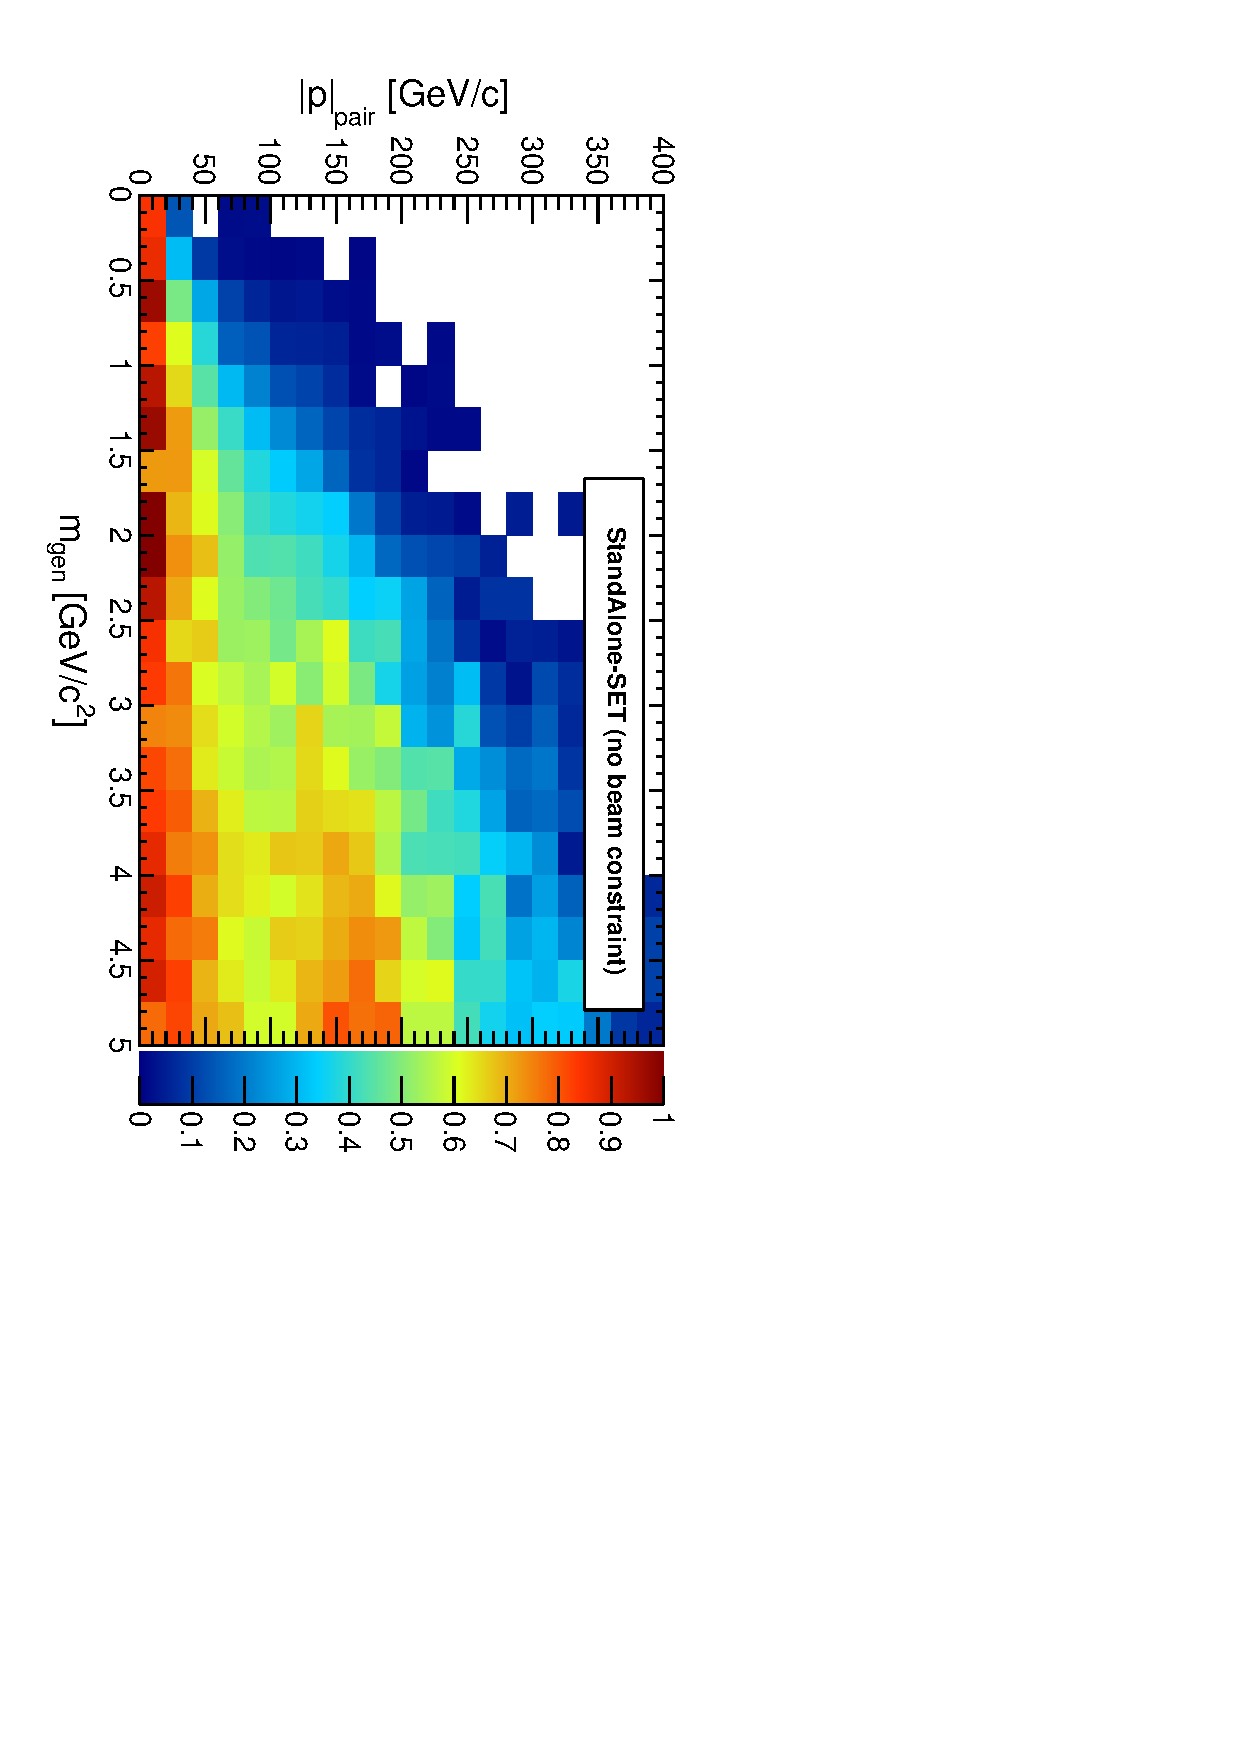
\includegraphics[height=0.5\linewidth, angle=90]{fig/acceptanceNoMCMatch_plot/pairpmagvsmass_StandAloneSET.pdf}

\caption{Same as Fig.~\ref{fig:pairpmagvsmass}, except that numerator only requires two reconstructed muons (no MC-matching).  \label{fig:pairpmagvsmassNoMCMatch}}
\end{figure}

\begin{figure}
\begin{center}
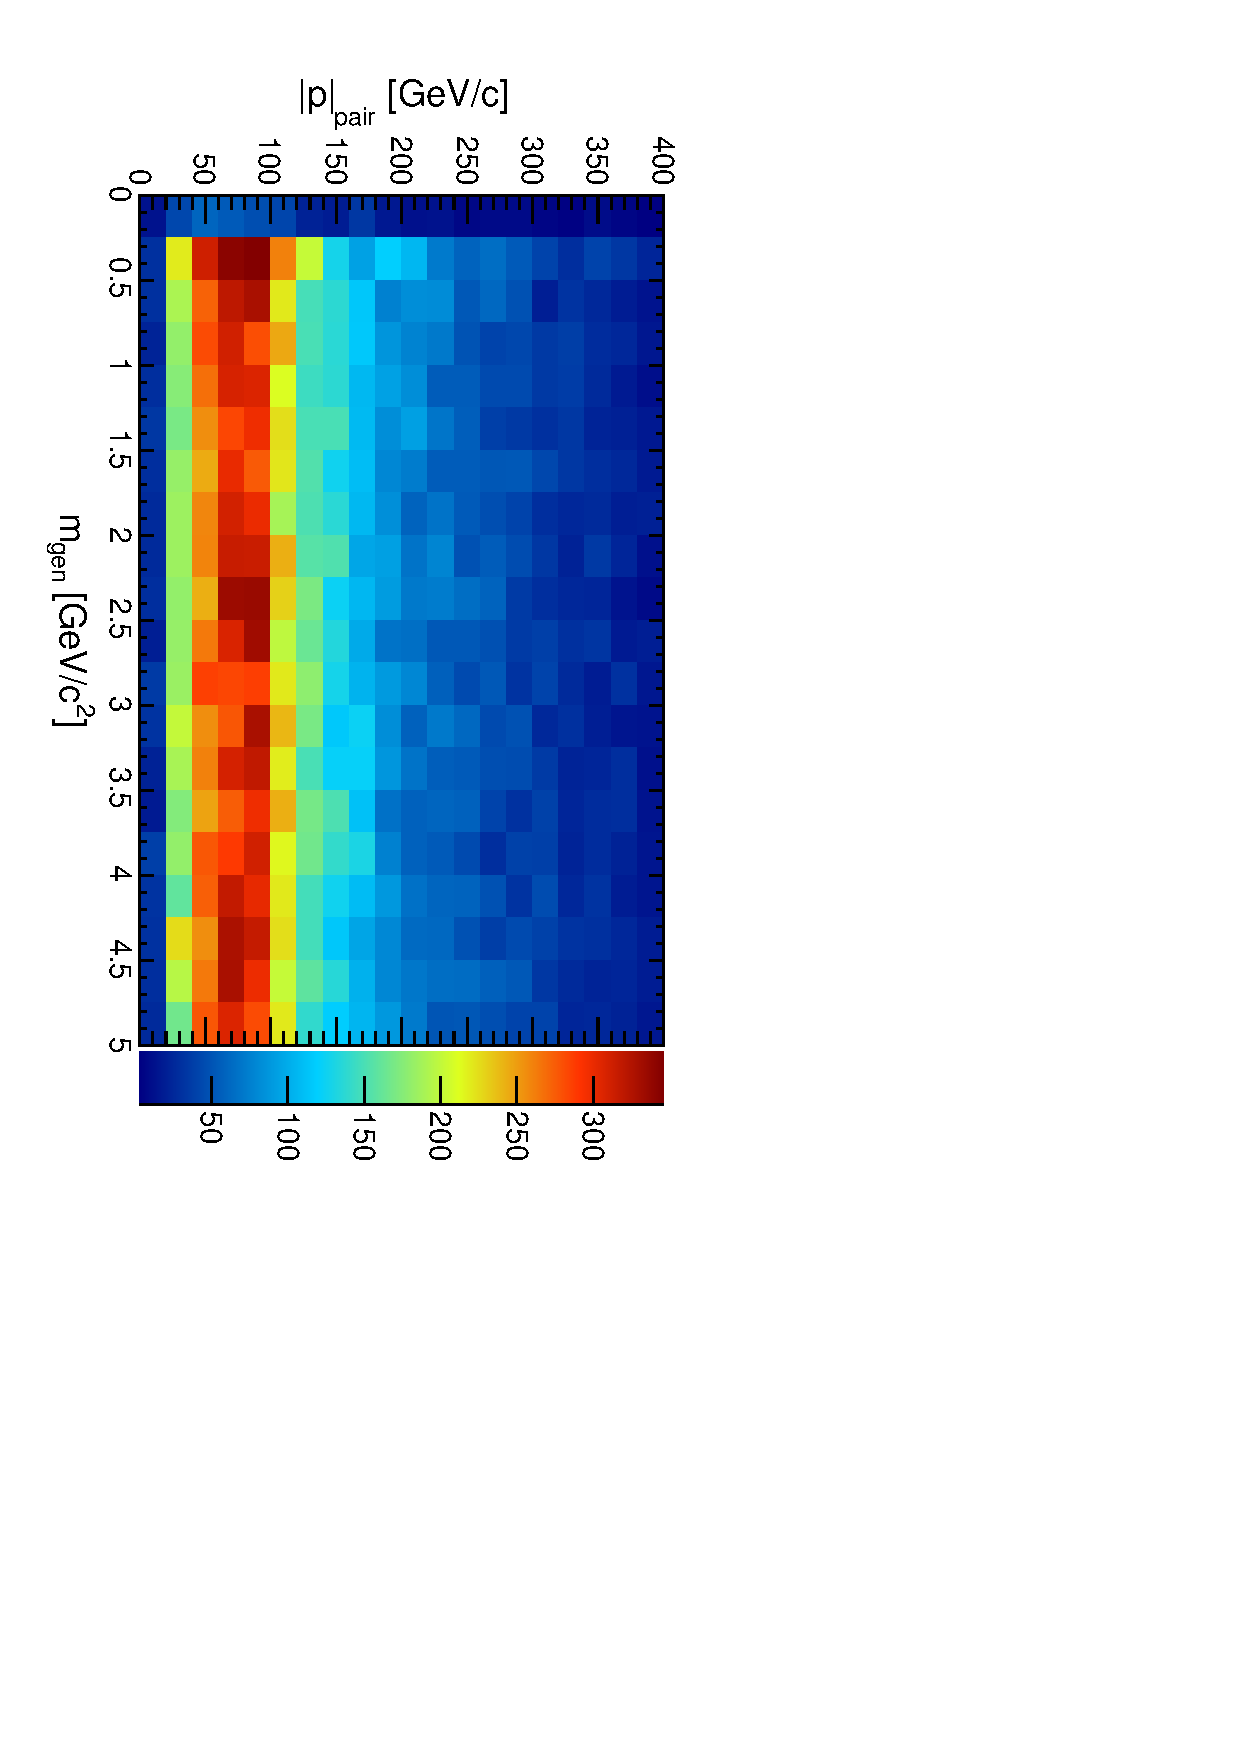
\includegraphics[height=0.5\linewidth, angle=90]{fig/acceptance_plot/pairpmagvsmass_TrackerMuons_denominator.pdf}
\end{center}
\caption{Denominator of plots in Figs.~\ref{fig:pairpmagvsmass} and \ref{fig:pairpmagvsmassNoMCMatch}.}
\end{figure}

\begin{figure}[p]
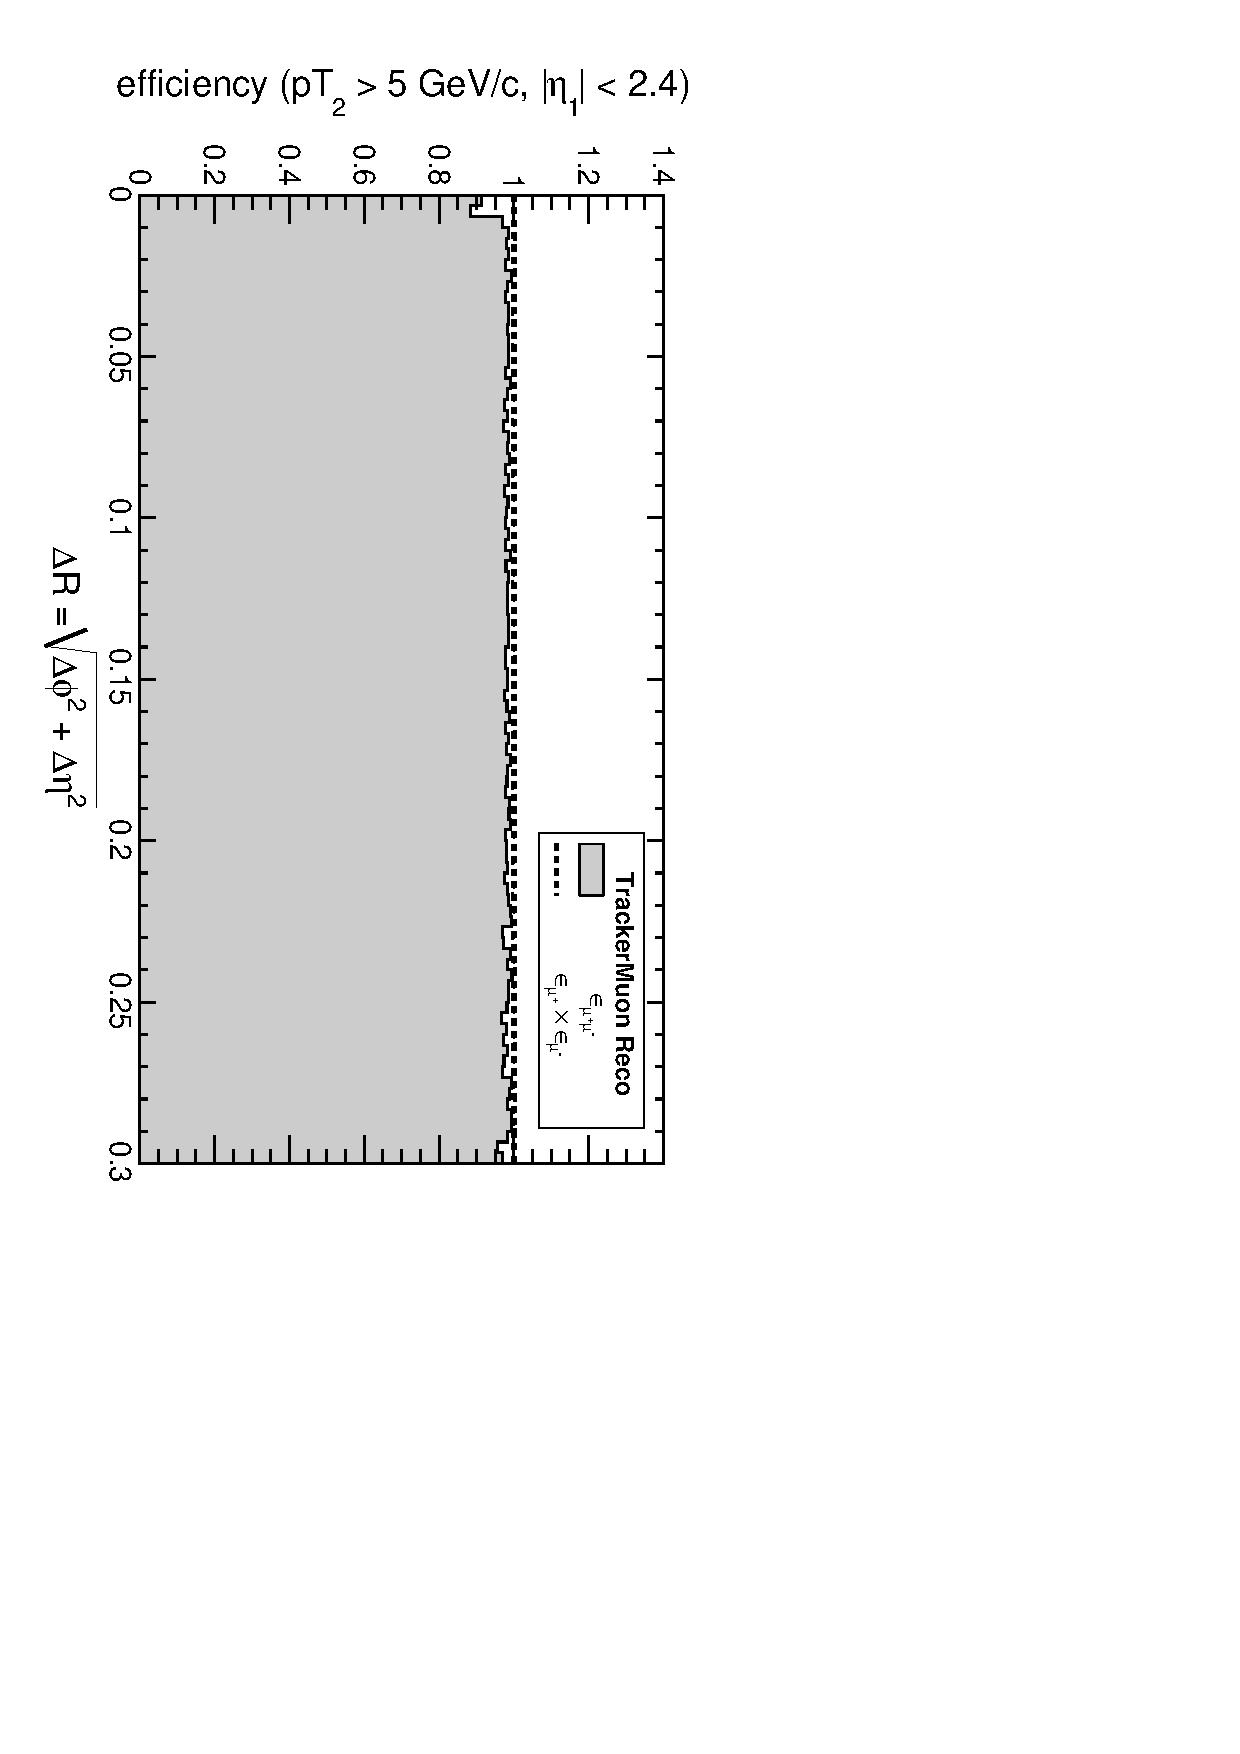
\includegraphics[height=0.5\linewidth, angle=90]{fig/acceptance6_plot/vsdR_TrackerMuons.pdf}
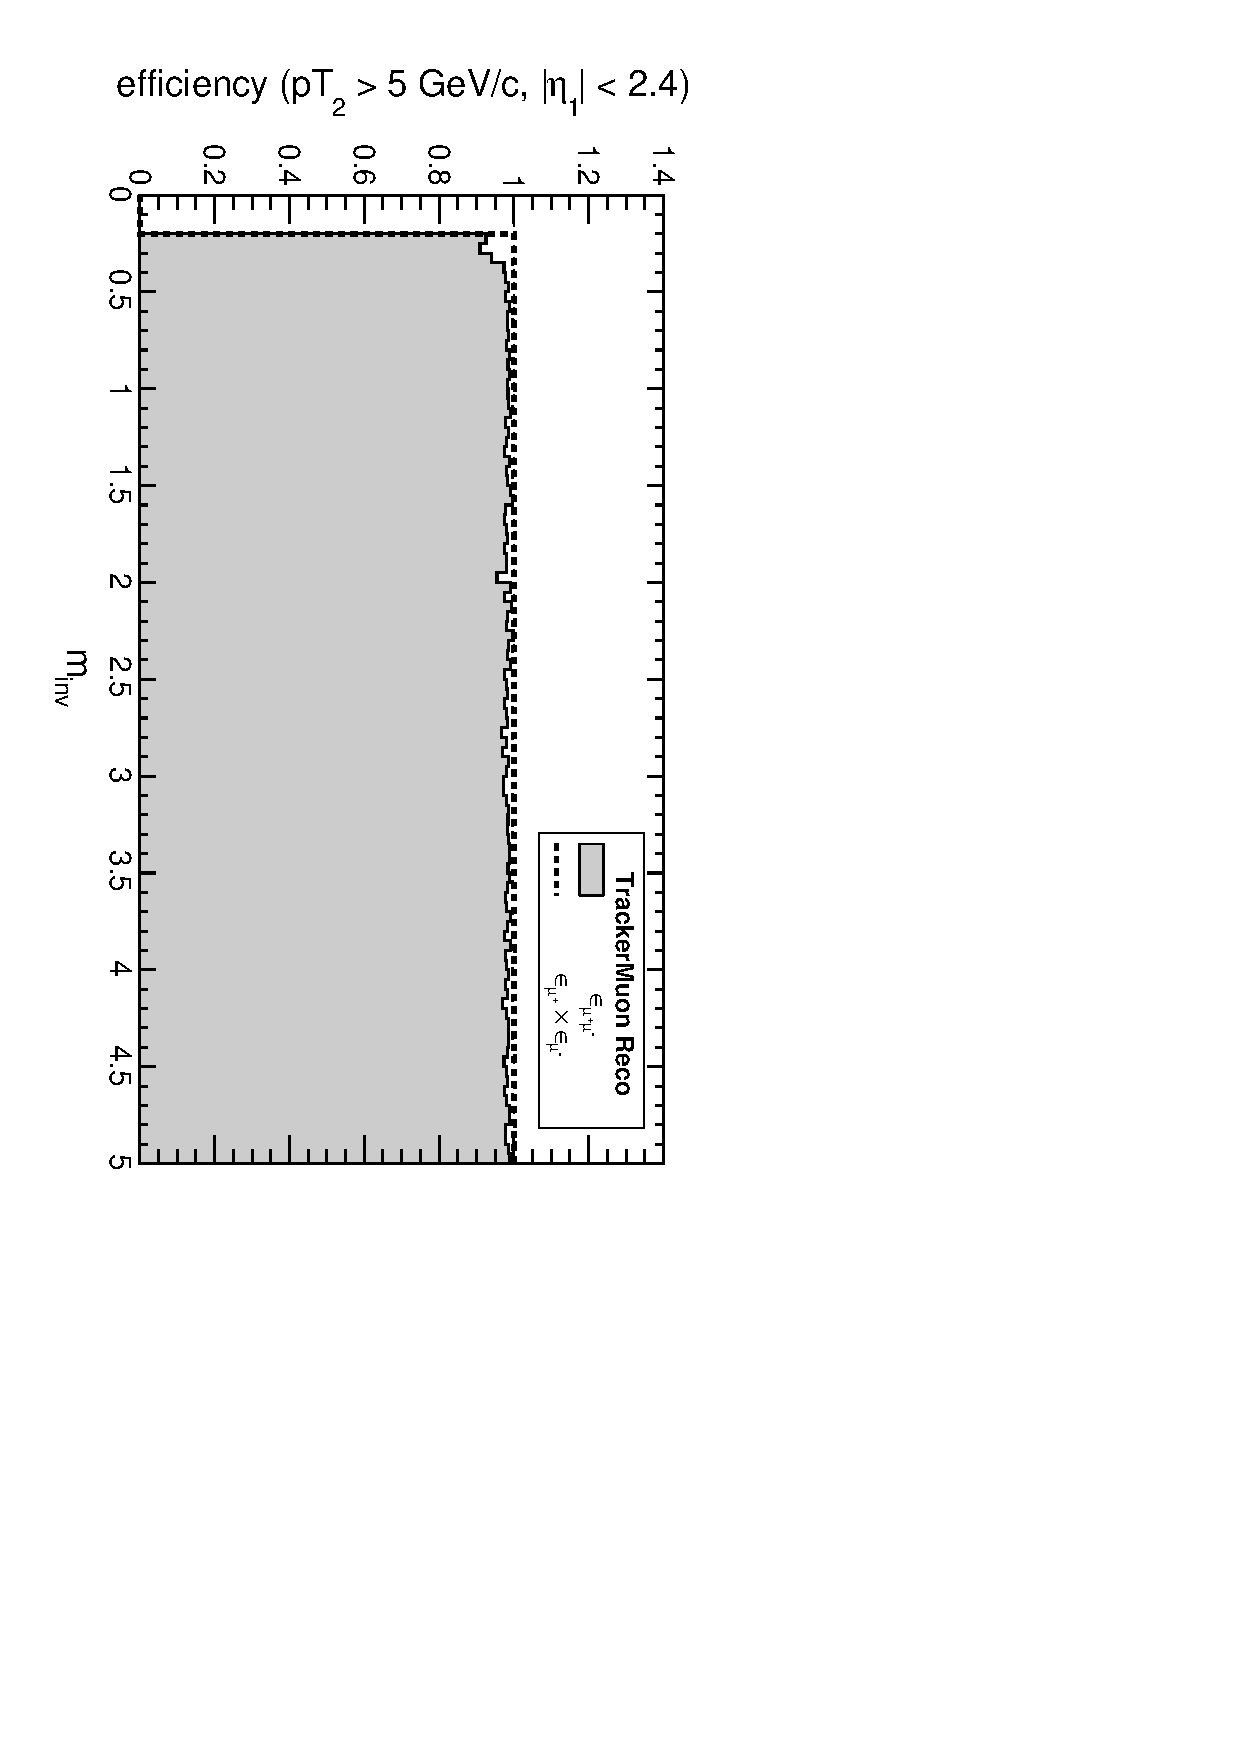
\includegraphics[height=0.5\linewidth, angle=90]{fig/acceptance6_plot/vsmass_TrackerMuons.pdf}

\caption{Reconstruction efficiency of TrackerMuons as a function of
  separation, compared with the product of efficiencies for the
  $\mu^+$ and $\mu^-$ alone. \label{fig:vseverything_TrackerMuons}}
\end{figure}

\begin{figure}[p]
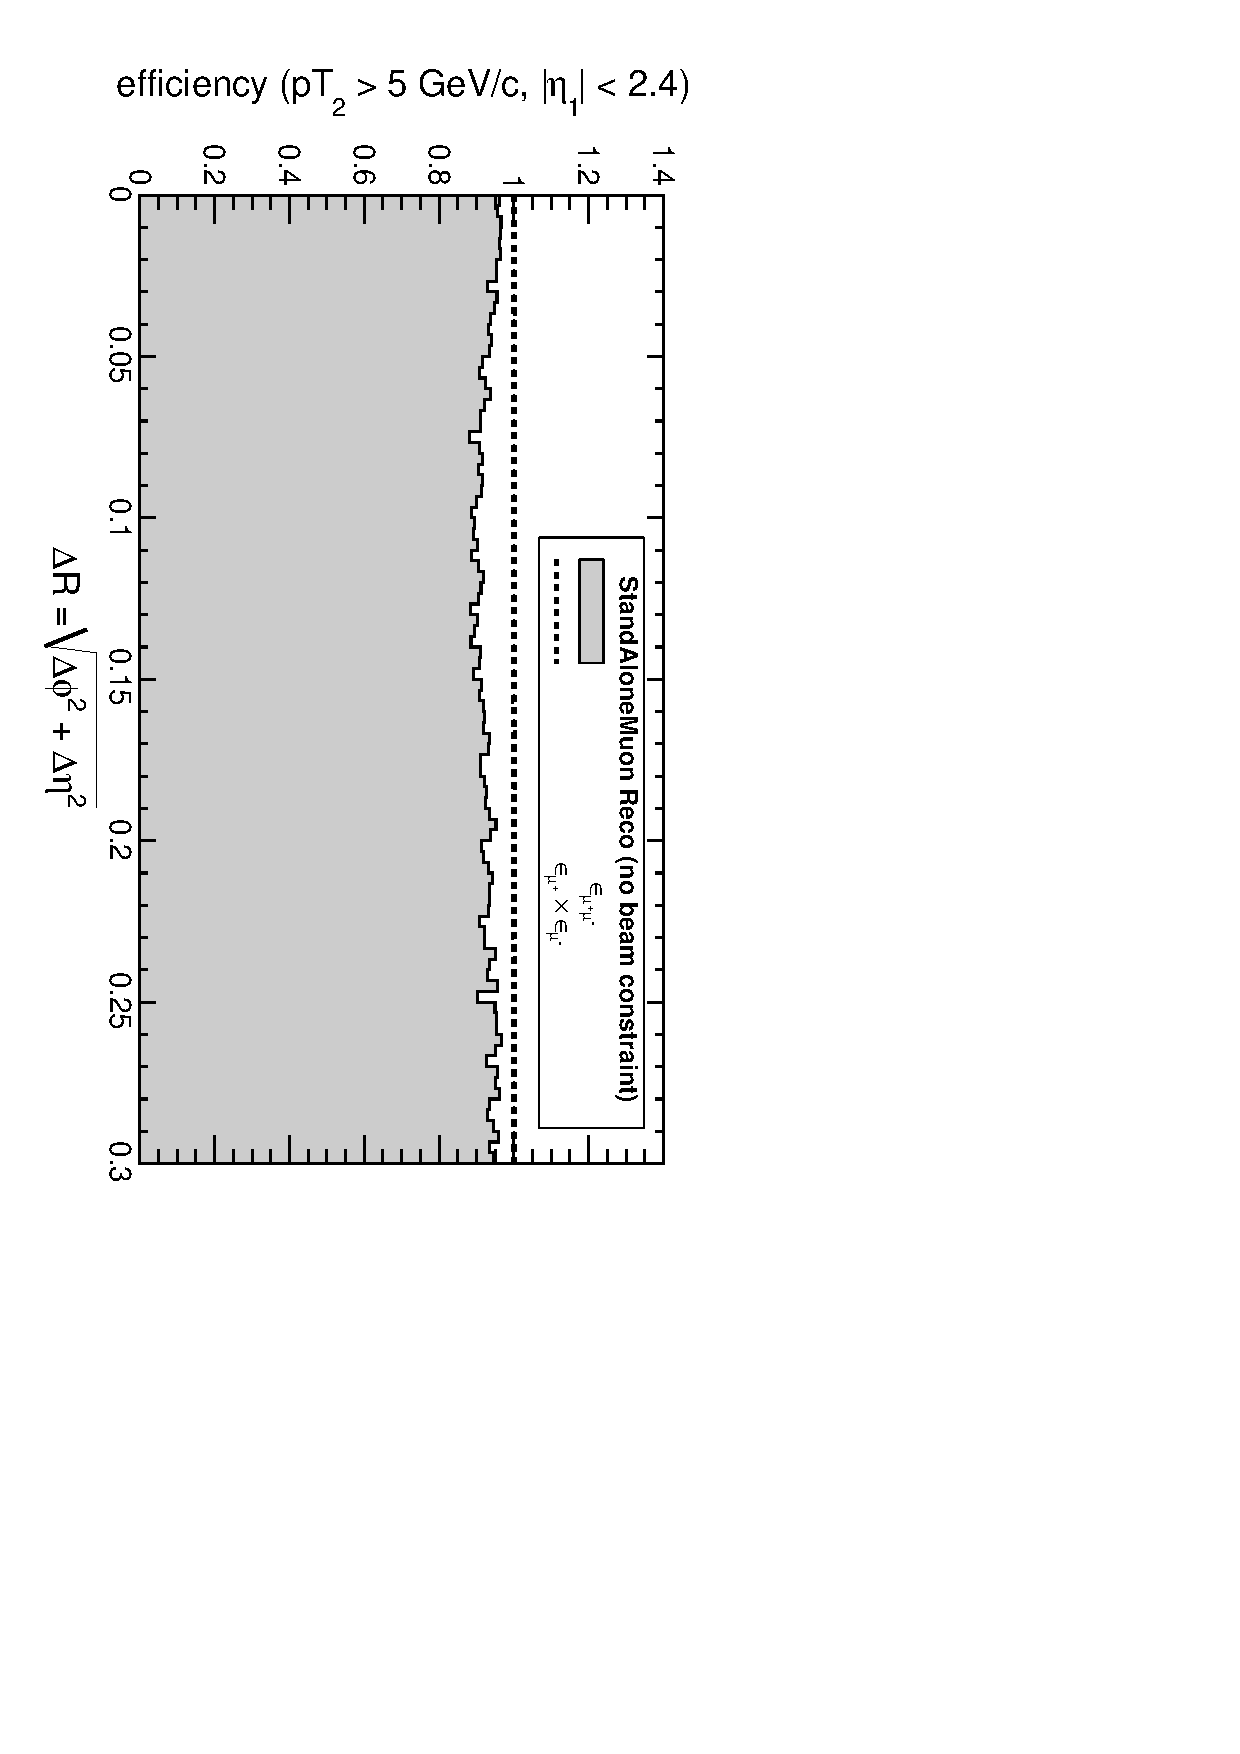
\includegraphics[height=0.5\linewidth, angle=90]{fig/acceptance6_plot/vsdR_StandAloneDefault.pdf}
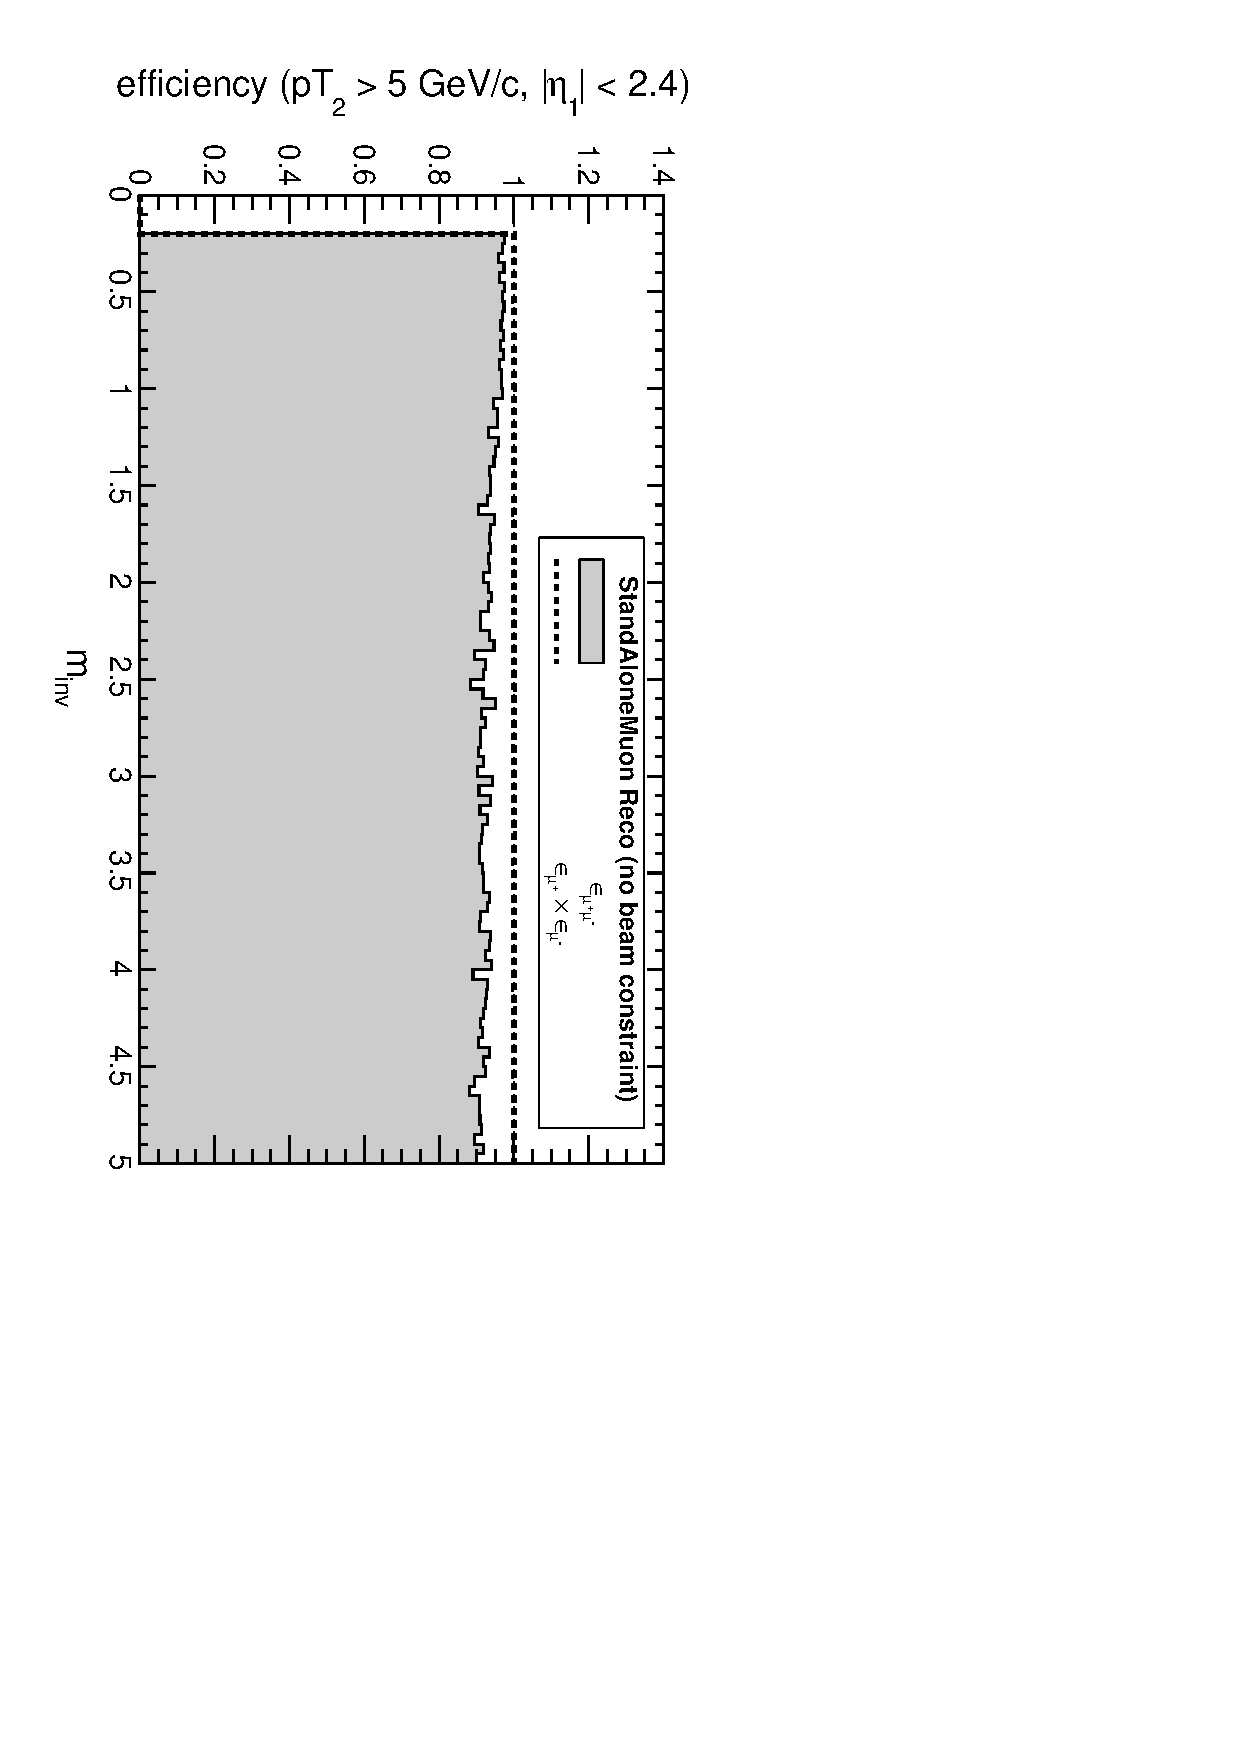
\includegraphics[height=0.5\linewidth, angle=90]{fig/acceptance6_plot/vsmass_StandAloneDefault.pdf}

\caption{Reconstruction efficiency of StandAloneMuons (no beamline constraint) as a function of
  separation, compared with the product of efficiencies for the
  $\mu^+$ and $\mu^-$ alone. \label{fig:vseverything_StandAloneDefault}}
\end{figure}

\begin{figure}[p]
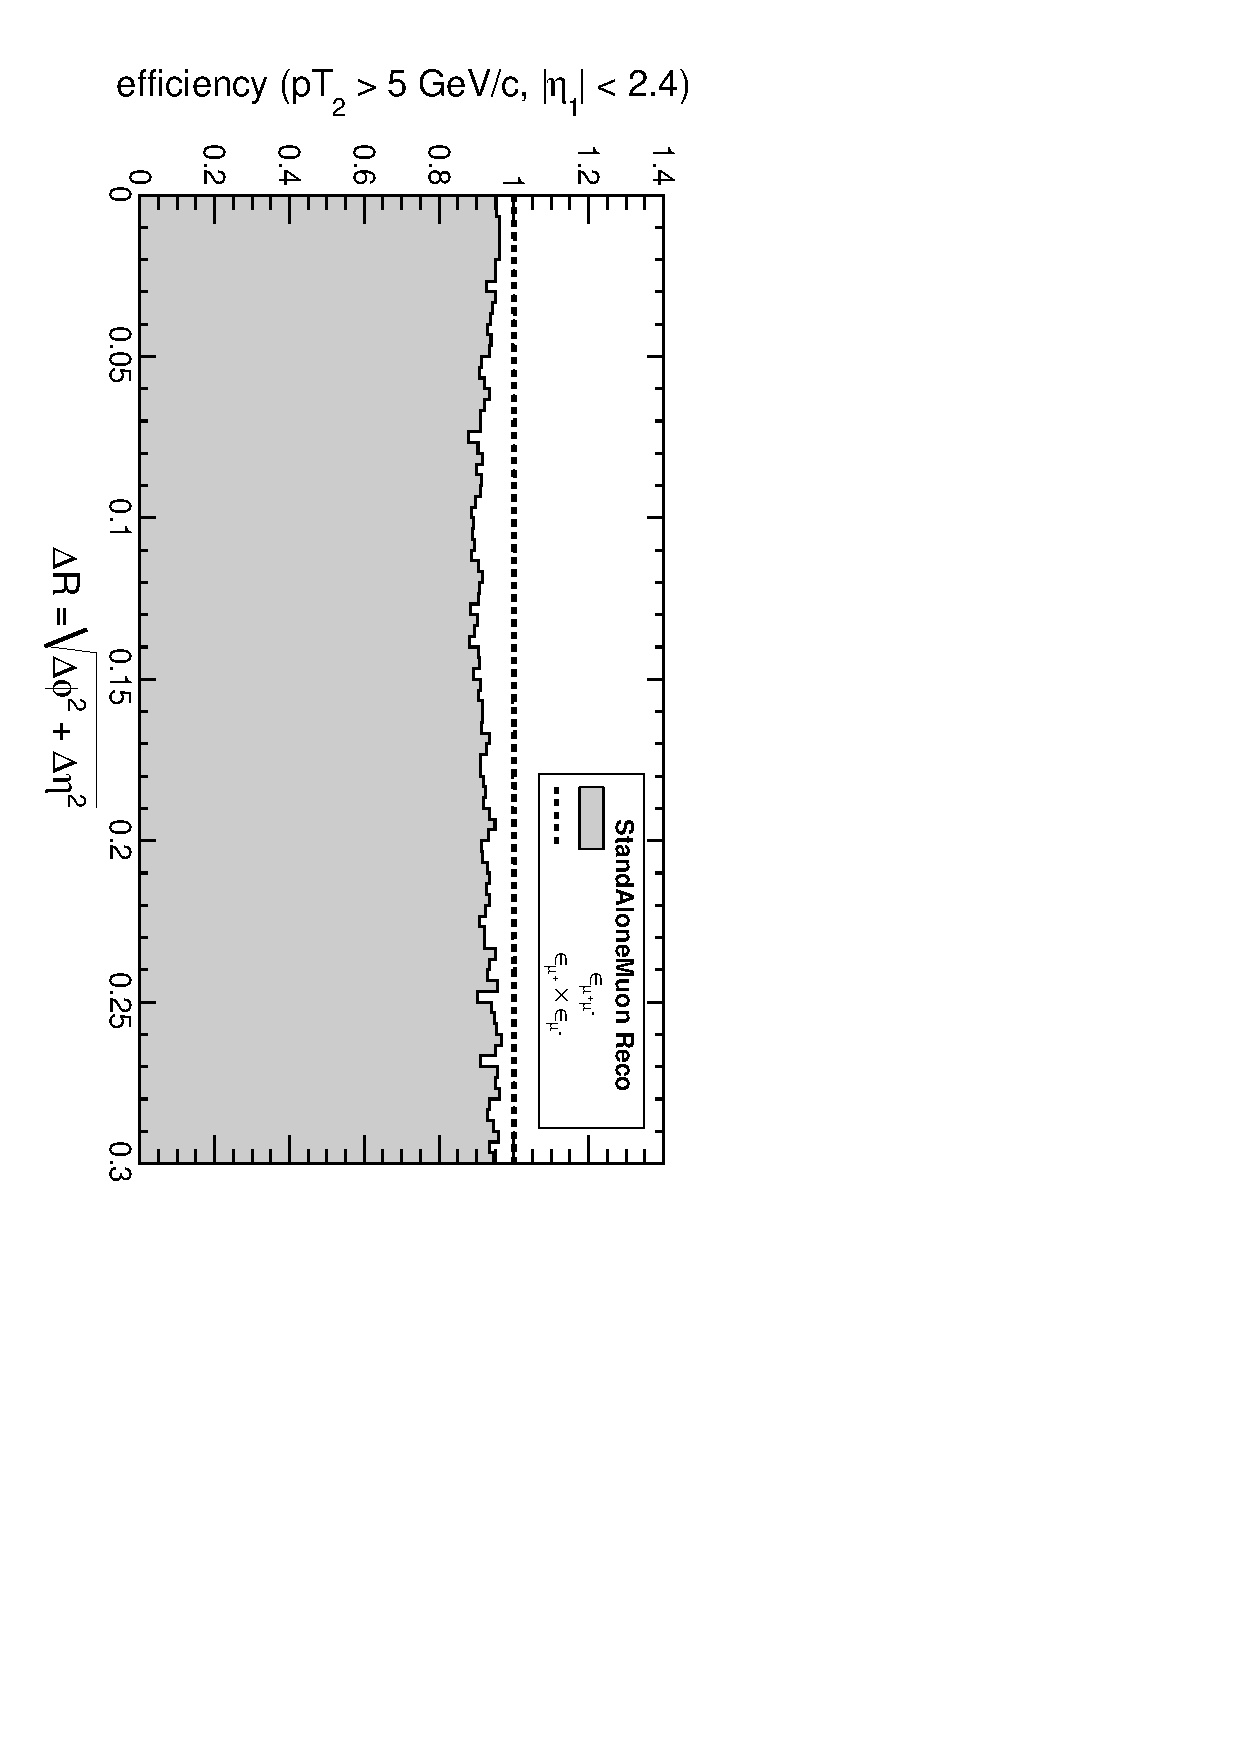
\includegraphics[height=0.5\linewidth, angle=90]{fig/acceptance6_plot/vsdR_StandAloneUpdatedDefault.pdf}
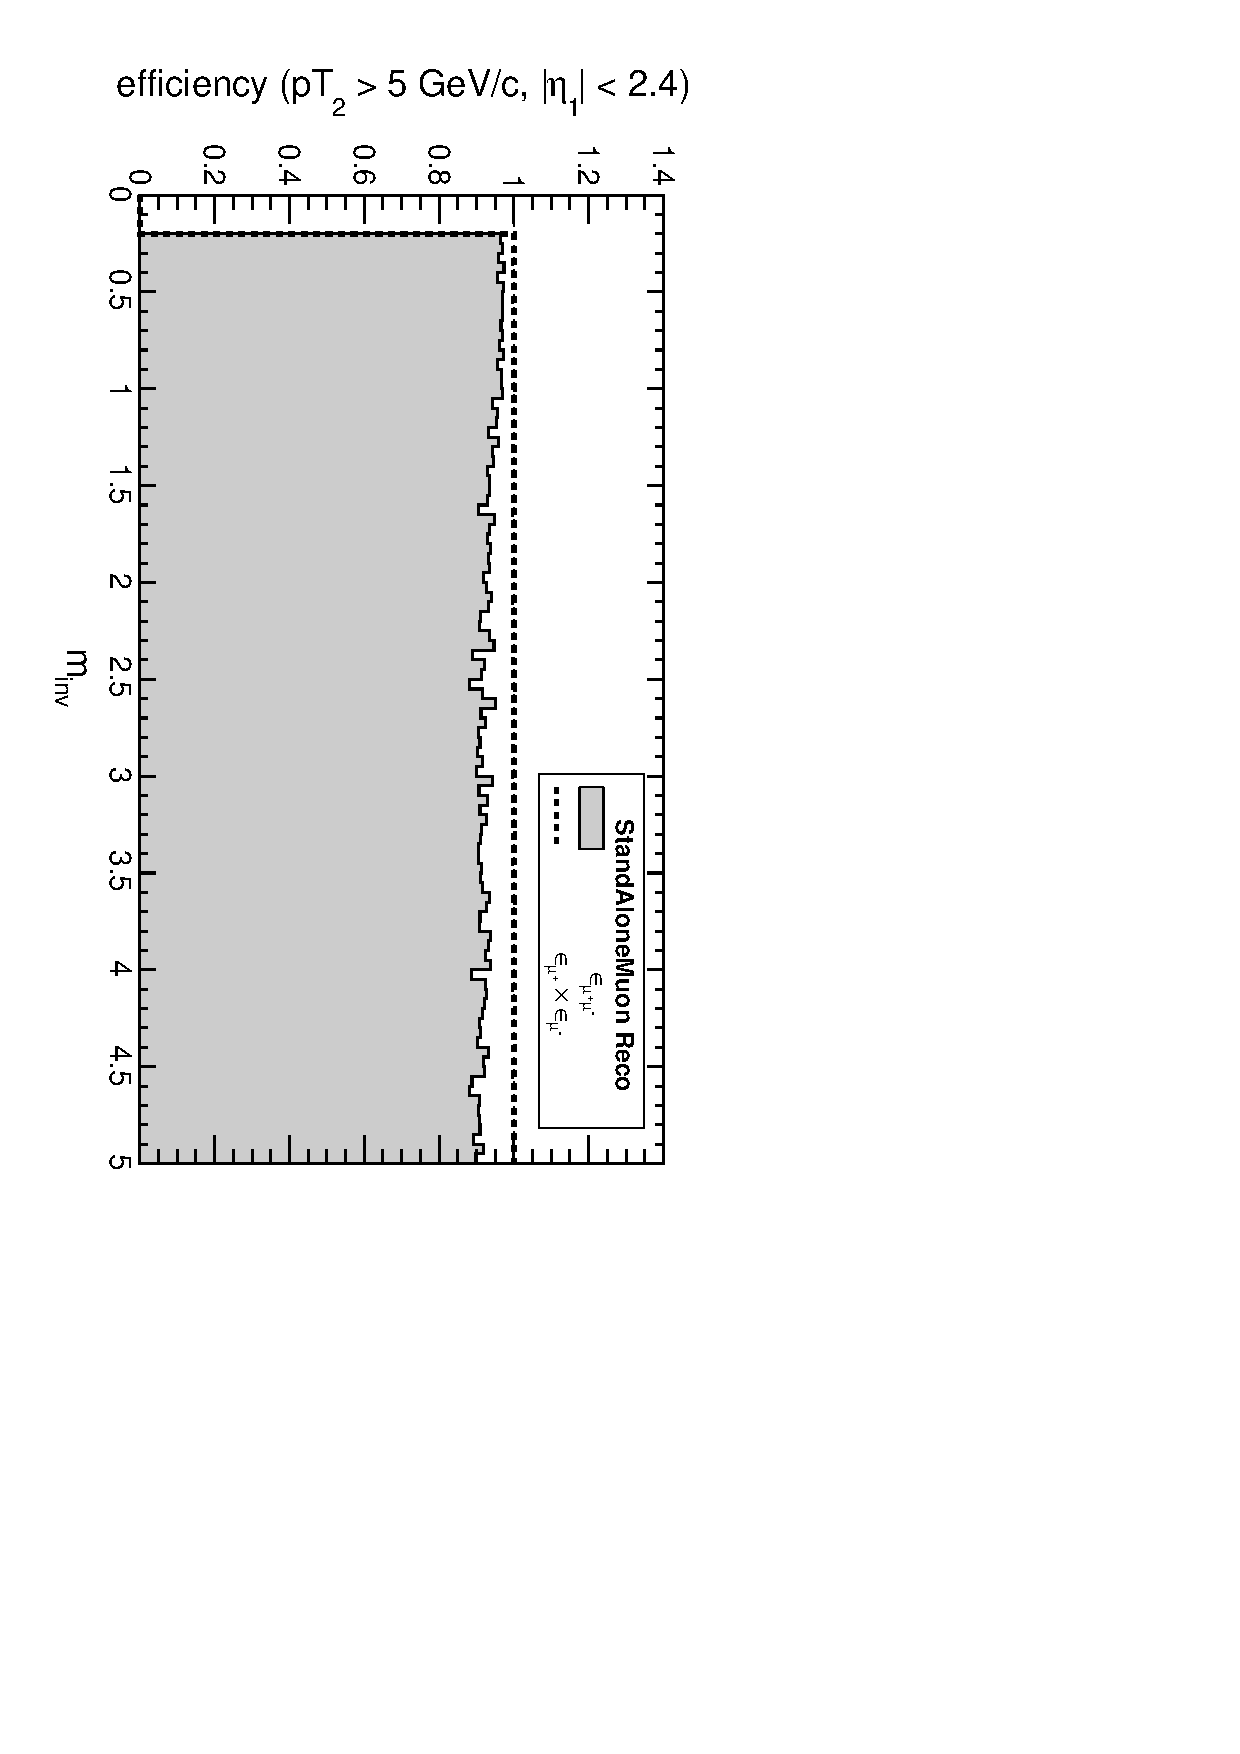
\includegraphics[height=0.5\linewidth, angle=90]{fig/acceptance6_plot/vsmass_StandAloneUpdatedDefault.pdf}

\caption{Reconstruction efficiency of StandAloneMuons (with beamline constraint) as a function of
  separation, compared with the product of efficiencies for the
  $\mu^+$ and $\mu^-$ alone. \label{fig:vseverything_StandAloneUpdatedDefault}}
\end{figure}

\begin{figure}[p]
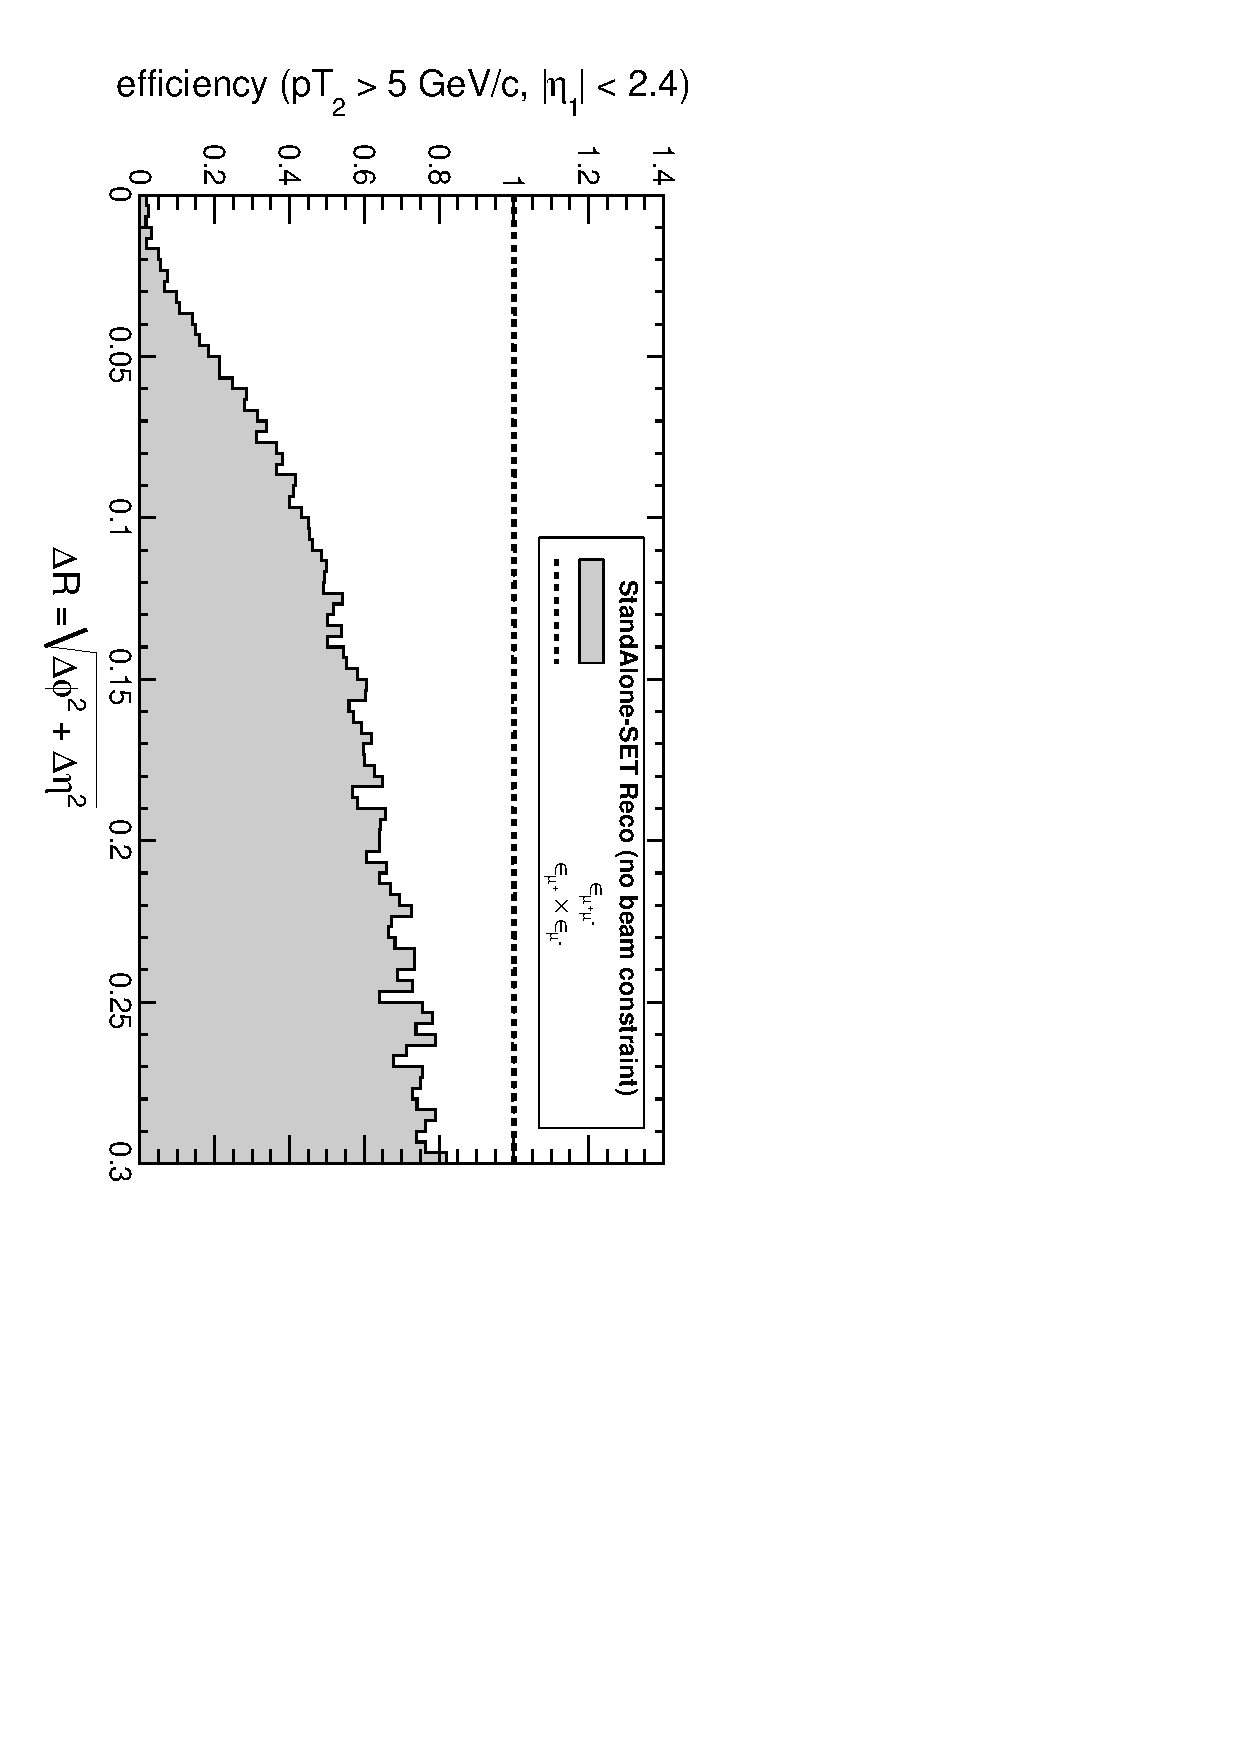
\includegraphics[height=0.5\linewidth, angle=90]{fig/acceptance6_plot/vsdR_StandAloneSET.pdf}
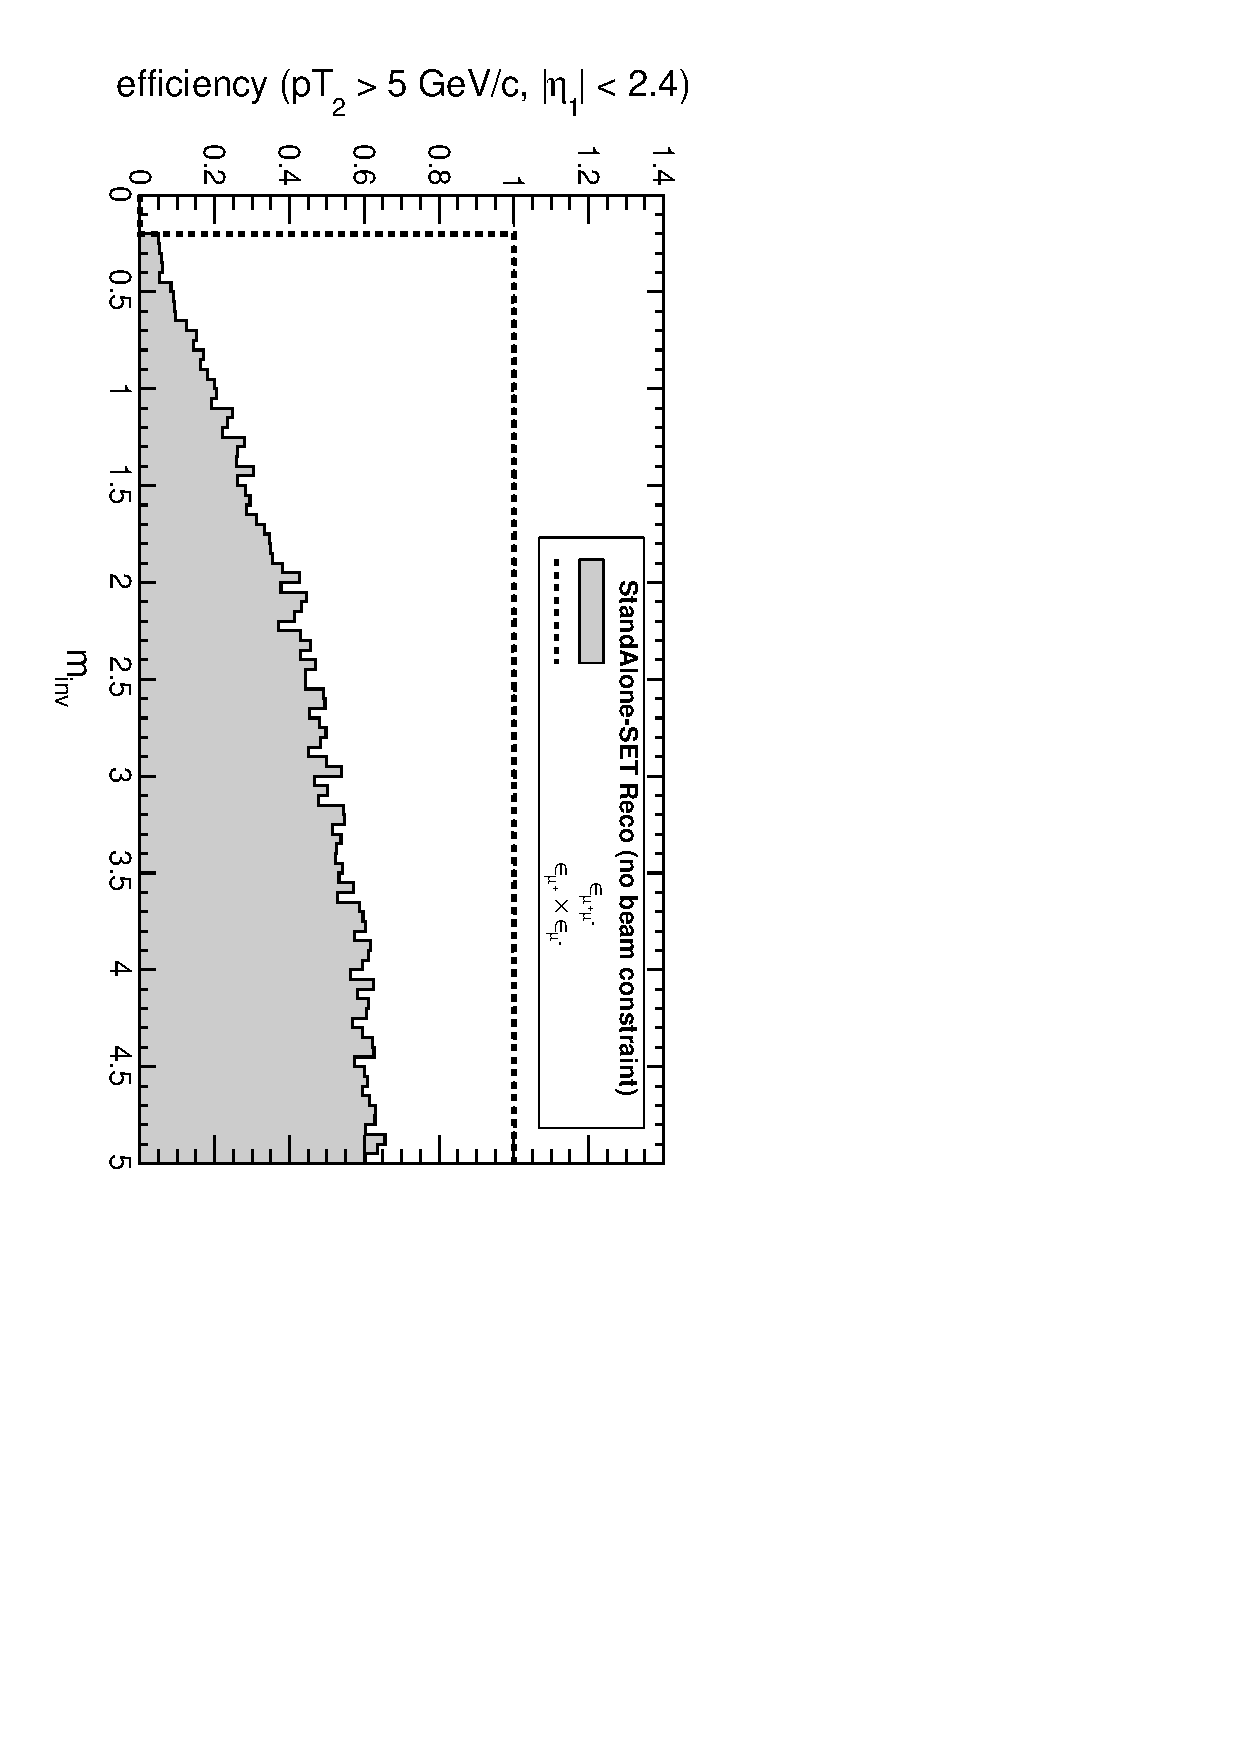
\includegraphics[height=0.5\linewidth, angle=90]{fig/acceptance6_plot/vsmass_StandAloneSET.pdf}

\caption{Reconstruction efficiency of StandAlone-SET muons (no beamline constraint) as a function of
  separation, compared with the product of efficiencies for the
  $\mu^+$ and $\mu^-$ alone. \label{fig:vseverything_StandAloneSET}}
\end{figure}

\begin{figure}[p]
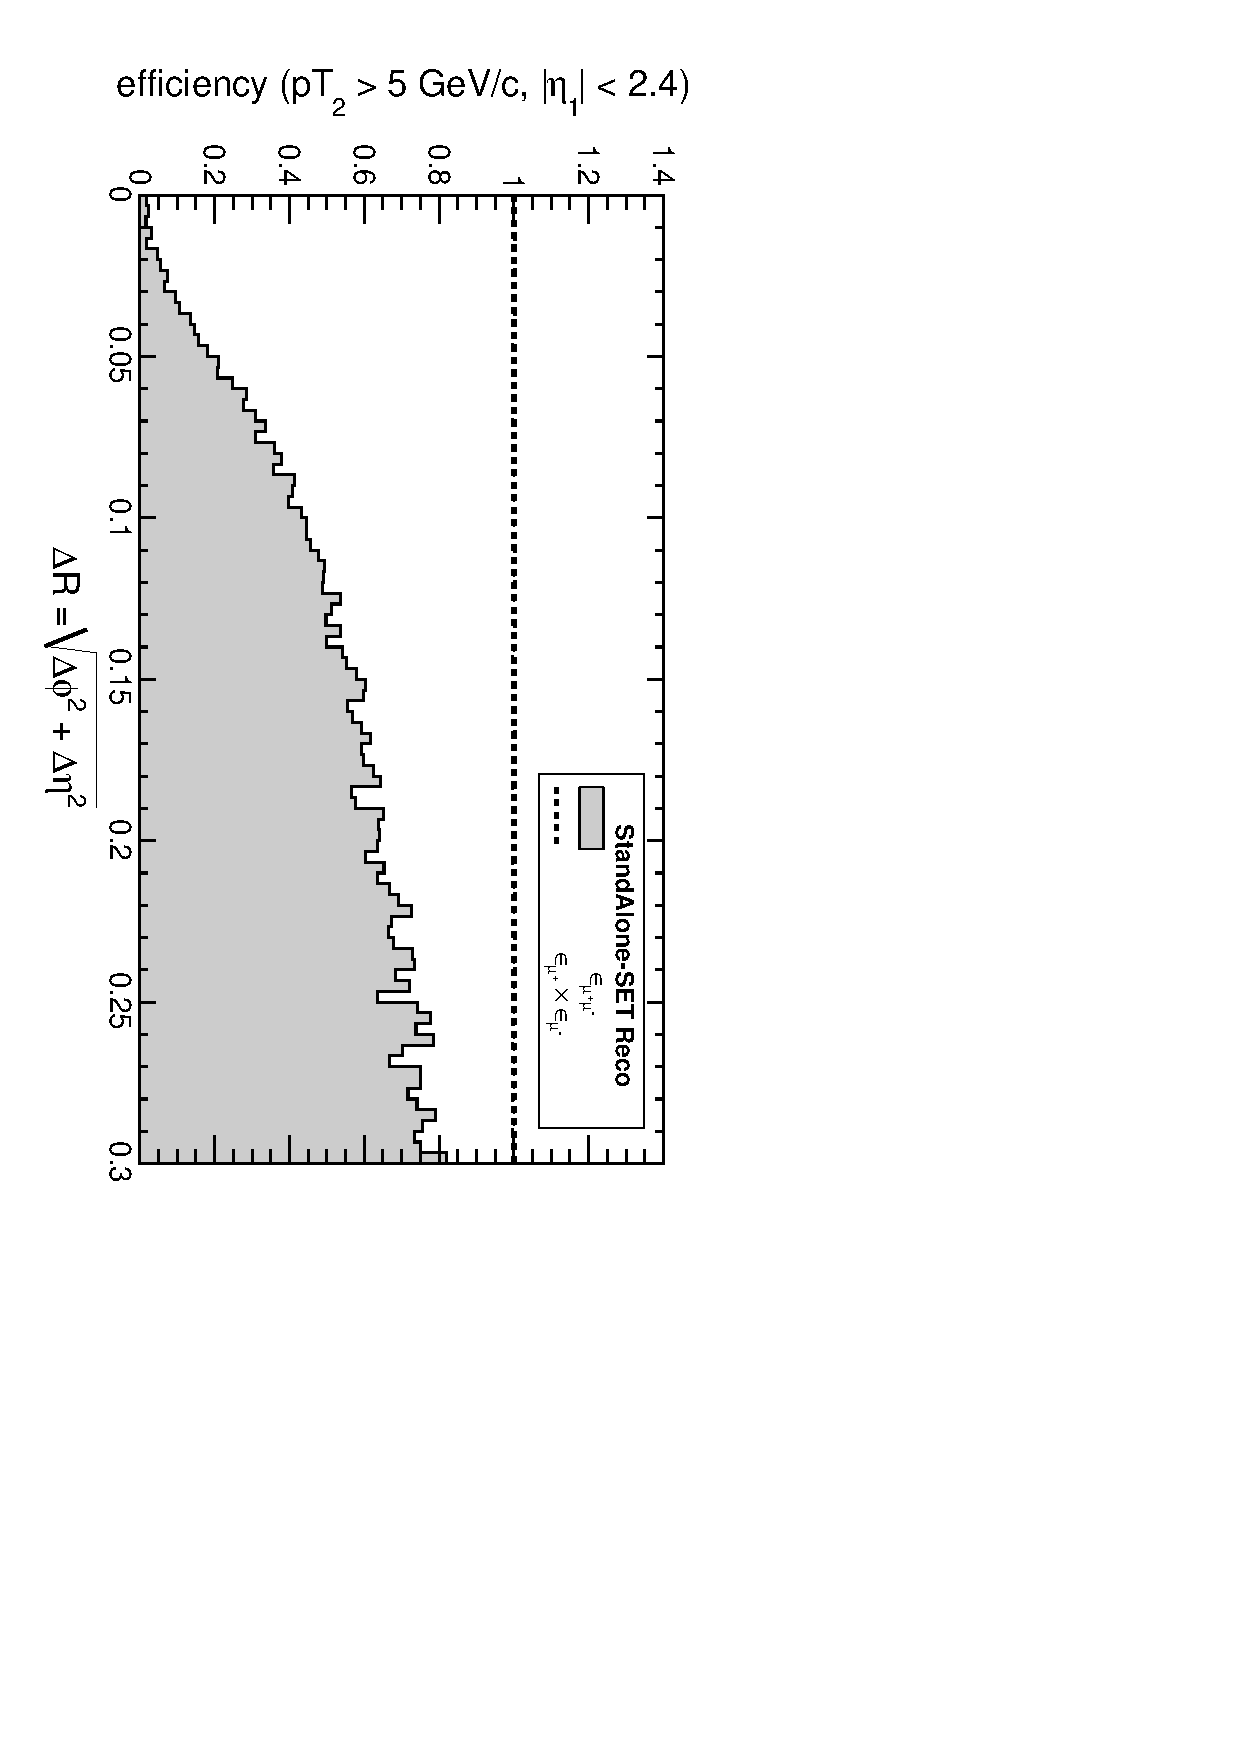
\includegraphics[height=0.5\linewidth, angle=90]{fig/acceptance6_plot/vsdR_StandAloneUpdatedSET.pdf}
\includegraphics[height=0.5\linewidth, angle=90]{fig/acceptance6_plot/vsmass_StandAloneUpdatedSET.pdf}

\caption{Reconstruction efficiency of StandAlone-SET muons (with beamline constraint) as a function of
  separation, compared with the product of efficiencies for the
  $\mu^+$ and $\mu^-$ alone. \label{fig:vseverything_StandAloneUpdatedSET}}
\end{figure}

\begin{figure}[p]
\includegraphics[height=0.5\linewidth, angle=90]{fig/acceptance6_plot/vsdR_GlobalMuons.pdf}
\includegraphics[height=0.5\linewidth, angle=90]{fig/acceptance6_plot/vsmass_GlobalMuons.pdf}

\caption{Reconstruction efficiency of GlobalMuons as a function of
  separation, compared with the product of efficiencies for the
  $\mu^+$ and $\mu^-$ alone. \label{fig:vseverything_GlobalMuons}}
\end{figure}

\clearpage

\begin{figure}[p]
\includegraphics[height=0.5\linewidth, angle=90]{fig/acceptance7_plot/mb1_TrackerMuons.pdf}
\includegraphics[height=0.5\linewidth, angle=90]{fig/acceptance7_plot/mb1_GlobalMuons.pdf}

\includegraphics[height=0.5\linewidth, angle=90]{fig/acceptance7_plot/mb1_StandAloneUpdatedDefault.pdf}
\includegraphics[height=0.5\linewidth, angle=90]{fig/acceptance7_plot/mb1_StandAloneDefault.pdf}

\includegraphics[height=0.5\linewidth, angle=90]{fig/acceptance7_plot/mb1_StandAloneUpdatedSET.pdf}
\includegraphics[height=0.5\linewidth, angle=90]{fig/acceptance7_plot/mb1_StandAloneSET.pdf}

\caption{Efficiency as a function of crossing in muon barrel
  station~1: $\Delta\phi_{MB1}$ and $\Delta Z_{MB1}$ are the azimuthal
  separation angle and longitudinal separation distance of the
  generator-level muon trajectories on a beam-aligned cylindrical
  surface with radius 432.946~cm ($\mu^+$ minus $\mu^-$).
  Denominator: generated events with $pT_2 > 5$~GeV/$c$ and $|\eta_1|
  < 2.4$ (mass ranges up to 50~GeV/$c^2$); numerator: reconstructed
  $\mu^+$ and $\mu^-$. \fixme{Barrel StandAlone/GlobalMuon
    inefficiencies are always off-center--- could this be an
    indication that the point of confusion in $|\eta| < 1.0$ is not in
    the muon chambers but somewhere nearby?  It looks like an image
    out-of-focus, like you overshot the location that drives the
    inefficiency.} \label{fig:mb1}}
\end{figure}

\begin{figure}[p]
\includegraphics[height=0.5\linewidth, angle=90]{fig/acceptance7_plot/mb2_TrackerMuons.pdf}
\includegraphics[height=0.5\linewidth, angle=90]{fig/acceptance7_plot/mb2_GlobalMuons.pdf}

\includegraphics[height=0.5\linewidth, angle=90]{fig/acceptance7_plot/mb2_StandAloneUpdatedDefault.pdf}
\includegraphics[height=0.5\linewidth, angle=90]{fig/acceptance7_plot/mb2_StandAloneDefault.pdf}

\includegraphics[height=0.5\linewidth, angle=90]{fig/acceptance7_plot/mb2_StandAloneUpdatedSET.pdf}
\includegraphics[height=0.5\linewidth, angle=90]{fig/acceptance7_plot/mb2_StandAloneSET.pdf}

\caption{Efficiency as a function of crossing in muon barrel
  station~2: $\Delta\phi_{MB2}$ and $\Delta Z_{MB2}$ are the azimuthal
  separation angle and longitudinal separation distance of the
  generator-level muon trajectories on a beam-aligned cylindrical
  surface with radius 512.923~cm ($\mu^+$ minus $\mu^-$).
  Denominator: generated events with $pT_2 > 5$~GeV/$c$ and $|\eta_1|
  < 2.4$ (mass ranges up to 50~GeV/$c^2$); numerator: reconstructed
  $\mu^+$ and $\mu^-$. \label{fig:mb2}}
\end{figure}

\begin{figure}[p]
\includegraphics[height=0.5\linewidth, angle=90]{fig/acceptance7_plot/mb3_TrackerMuons.pdf}
\includegraphics[height=0.5\linewidth, angle=90]{fig/acceptance7_plot/mb3_GlobalMuons.pdf}

\includegraphics[height=0.5\linewidth, angle=90]{fig/acceptance7_plot/mb3_StandAloneUpdatedDefault.pdf}
\includegraphics[height=0.5\linewidth, angle=90]{fig/acceptance7_plot/mb3_StandAloneDefault.pdf}

\includegraphics[height=0.5\linewidth, angle=90]{fig/acceptance7_plot/mb3_StandAloneUpdatedSET.pdf}
\includegraphics[height=0.5\linewidth, angle=90]{fig/acceptance7_plot/mb3_StandAloneSET.pdf}

\caption{Efficiency as a function of crossing in muon barrel
  station~3: $\Delta\phi_{MB3}$ and $\Delta Z_{MB3}$ are the azimuthal
  separation angle and longitudinal separation distance of the
  generator-level muon trajectories on a beam-aligned cylindrical
  surface with radius 618.269~cm ($\mu^+$ minus $\mu^-$).
  Denominator: generated events with $pT_2 > 5$~GeV/$c$ and $|\eta_1|
  < 2.4$ (mass ranges up to 50~GeV/$c^2$); numerator: reconstructed
  $\mu^+$ and $\mu^-$. \label{fig:mb3}}
\end{figure}

\begin{figure}[p]
\includegraphics[height=0.5\linewidth, angle=90]{fig/acceptance7_plot/mb4_TrackerMuons.pdf}
\includegraphics[height=0.5\linewidth, angle=90]{fig/acceptance7_plot/mb4_GlobalMuons.pdf}

\includegraphics[height=0.5\linewidth, angle=90]{fig/acceptance7_plot/mb4_StandAloneUpdatedDefault.pdf}
\includegraphics[height=0.5\linewidth, angle=90]{fig/acceptance7_plot/mb4_StandAloneDefault.pdf}

\includegraphics[height=0.5\linewidth, angle=90]{fig/acceptance7_plot/mb4_StandAloneUpdatedSET.pdf}
\includegraphics[height=0.5\linewidth, angle=90]{fig/acceptance7_plot/mb4_StandAloneSET.pdf}

\caption{Efficiency as a function of crossing in muon barrel
  station~4: $\Delta\phi_{MB4}$ and $\Delta Z_{MB4}$ are the azimuthal
  separation angle and longitudinal separation distance of the
  generator-level muon trajectories on a beam-aligned cylindrical
  surface with radius 726.425~cm ($\mu^+$ minus $\mu^-$).
  Denominator: generated events with $pT_2 > 5$~GeV/$c$ and $|\eta_1|
  < 2.4$ (mass ranges up to 50~GeV/$c^2$); numerator: reconstructed
  $\mu^+$ and $\mu^-$. \label{fig:mb4}}
\end{figure}

\clearpage

\begin{figure}[p]
\includegraphics[height=0.5\linewidth, angle=90]{fig/acceptance7_plot/me11_TrackerMuons.pdf}
\includegraphics[height=0.5\linewidth, angle=90]{fig/acceptance7_plot/me11_GlobalMuons.pdf}

\includegraphics[height=0.5\linewidth, angle=90]{fig/acceptance7_plot/me11_StandAloneUpdatedDefault.pdf}
\includegraphics[height=0.5\linewidth, angle=90]{fig/acceptance7_plot/me11_StandAloneDefault.pdf}

\includegraphics[height=0.5\linewidth, angle=90]{fig/acceptance7_plot/me11_StandAloneUpdatedSET.pdf}
\includegraphics[height=0.5\linewidth, angle=90]{fig/acceptance7_plot/me11_StandAloneSET.pdf}

\caption{Efficiency as a function of crossing in muon endcap station
  ME1/1: $\Delta\phi_{ME1/1}$ and $\Delta R_{ME1/1}$ are the azimuthal
  separation angle and radial separation distance of the
  generator-level muon trajectories on a plane transverse to the
  beamline at $\pm$602.3~cm ($\mu^+$ minus $\mu^-$).  Denominator:
  generated events with $pT_2 > 5$~GeV/$c$ and $|\eta_1| < 2.4$ (mass
  ranges up to 50~GeV/$c^2$); numerator: reconstructed $\mu^+$ and
  $\mu^-$. \fixme{Aysen recommends a different symbol than ``$\Delta
    R$''.} \label{fig:me11}}
\end{figure}

\begin{figure}[p]
\includegraphics[height=0.5\linewidth, angle=90]{fig/acceptance7_plot/me12_TrackerMuons.pdf}
\includegraphics[height=0.5\linewidth, angle=90]{fig/acceptance7_plot/me12_GlobalMuons.pdf}

\includegraphics[height=0.5\linewidth, angle=90]{fig/acceptance7_plot/me12_StandAloneUpdatedDefault.pdf}
\includegraphics[height=0.5\linewidth, angle=90]{fig/acceptance7_plot/me12_StandAloneDefault.pdf}

\includegraphics[height=0.5\linewidth, angle=90]{fig/acceptance7_plot/me12_StandAloneUpdatedSET.pdf}
\includegraphics[height=0.5\linewidth, angle=90]{fig/acceptance7_plot/me12_StandAloneSET.pdf}

\caption{Efficiency as a function of crossing in muon endcap station
  ME1/2: $\Delta\phi_{ME1/2}$ and $\Delta R_{ME1/2}$ are the azimuthal
  separation angle and radial separation distance of the
  generator-level muon trajectories on a plane transverse to the
  beamline at $\pm$699.061~cm ($\mu^+$ minus $\mu^-$).  Denominator:
  generated events with $pT_2 > 5$~GeV/$c$ and $|\eta_1| < 2.4$ (mass
  ranges up to 50~GeV/$c^2$); numerator: reconstructed $\mu^+$ and
  $\mu^-$. \label{fig:me12}}
\end{figure}

\begin{figure}[p]
\includegraphics[height=0.5\linewidth, angle=90]{fig/acceptance7_plot/me13_TrackerMuons.pdf}
\includegraphics[height=0.5\linewidth, angle=90]{fig/acceptance7_plot/me13_GlobalMuons.pdf}

\includegraphics[height=0.5\linewidth, angle=90]{fig/acceptance7_plot/me13_StandAloneUpdatedDefault.pdf}
\includegraphics[height=0.5\linewidth, angle=90]{fig/acceptance7_plot/me13_StandAloneDefault.pdf}

\includegraphics[height=0.5\linewidth, angle=90]{fig/acceptance7_plot/me13_StandAloneUpdatedSET.pdf}
\includegraphics[height=0.5\linewidth, angle=90]{fig/acceptance7_plot/me13_StandAloneSET.pdf}

\caption{Efficiency as a function of crossing in muon endcap station
  ME1/3: $\Delta\phi_{ME1/3}$ and $\Delta R_{ME1/3}$ are the azimuthal
  separation angle and radial separation distance of the
  generator-level muon trajectories on a plane transverse to the
  beamline at $\pm$695.159~cm ($\mu^+$ minus $\mu^-$).  Denominator:
  generated events with $pT_2 > 5$~GeV/$c$ and $|\eta_1| < 2.4$ (mass
  ranges up to 50~GeV/$c^2$); numerator: reconstructed $\mu^+$ and
  $\mu^-$. \label{fig:me13}}
\end{figure}

\begin{figure}[p]
\includegraphics[height=0.5\linewidth, angle=90]{fig/acceptance7_plot/me2_TrackerMuons.pdf}
\includegraphics[height=0.5\linewidth, angle=90]{fig/acceptance7_plot/me2_GlobalMuons.pdf}

\includegraphics[height=0.5\linewidth, angle=90]{fig/acceptance7_plot/me2_StandAloneUpdatedDefault.pdf}
\includegraphics[height=0.5\linewidth, angle=90]{fig/acceptance7_plot/me2_StandAloneDefault.pdf}

\includegraphics[height=0.5\linewidth, angle=90]{fig/acceptance7_plot/me2_StandAloneUpdatedSET.pdf}
\includegraphics[height=0.5\linewidth, angle=90]{fig/acceptance7_plot/me2_StandAloneSET.pdf}

\caption{Efficiency as a function of crossing in muon endcap station
  ME2: $\Delta\phi_{ME2}$ and $\Delta R_{ME2}$ are the azimuthal
  separation angle and radial separation distance of the
  generator-level muon trajectories on a plane transverse to the
  beamline at $\pm$828.561~cm ($\mu^+$ minus $\mu^-$).  Denominator:
  generated events with $pT_2 > 5$~GeV/$c$ and $|\eta_1| < 2.4$ (mass
  ranges up to 50~GeV/$c^2$); numerator: reconstructed $\mu^+$ and
  $\mu^-$. \label{fig:me2}}
\end{figure}

\begin{figure}[p]
\includegraphics[height=0.5\linewidth, angle=90]{fig/acceptance7_plot/me3_TrackerMuons.pdf}
\includegraphics[height=0.5\linewidth, angle=90]{fig/acceptance7_plot/me3_GlobalMuons.pdf}

\includegraphics[height=0.5\linewidth, angle=90]{fig/acceptance7_plot/me3_StandAloneUpdatedDefault.pdf}
\includegraphics[height=0.5\linewidth, angle=90]{fig/acceptance7_plot/me3_StandAloneDefault.pdf}

\includegraphics[height=0.5\linewidth, angle=90]{fig/acceptance7_plot/me3_StandAloneUpdatedSET.pdf}
\includegraphics[height=0.5\linewidth, angle=90]{fig/acceptance7_plot/me3_StandAloneSET.pdf}

\caption{Efficiency as a function of crossing in muon endcap station
  ME3: $\Delta\phi_{ME3}$ and $\Delta R_{ME3}$ are the azimuthal
  separation angle and radial separation distance of the
  generator-level muon trajectories on a plane transverse to the
  beamline at $\pm$935.439~cm ($\mu^+$ minus $\mu^-$).  Denominator:
  generated events with $pT_2 > 5$~GeV/$c$ and $|\eta_1| < 2.4$ (mass
  ranges up to 50~GeV/$c^2$); numerator: reconstructed $\mu^+$ and
  $\mu^-$. \label{fig:me3}}
\end{figure}

\begin{figure}[p]
\includegraphics[height=0.5\linewidth, angle=90]{fig/acceptance7_plot/me4_TrackerMuons.pdf}
\includegraphics[height=0.5\linewidth, angle=90]{fig/acceptance7_plot/me4_GlobalMuons.pdf}

\includegraphics[height=0.5\linewidth, angle=90]{fig/acceptance7_plot/me4_StandAloneUpdatedDefault.pdf}
\includegraphics[height=0.5\linewidth, angle=90]{fig/acceptance7_plot/me4_StandAloneDefault.pdf}

\includegraphics[height=0.5\linewidth, angle=90]{fig/acceptance7_plot/me4_StandAloneUpdatedSET.pdf}
\includegraphics[height=0.5\linewidth, angle=90]{fig/acceptance7_plot/me4_StandAloneSET.pdf}

\caption{Efficiency as a function of crossing in muon endcap station
  ME4: $\Delta\phi_{ME4}$ and $\Delta R_{ME4}$ are the azimuthal
  separation angle and radial separation distance of the
  generator-level muon trajectories on a plane transverse to the
  beamline at $\pm$1024.94~cm ($\mu^+$ minus $\mu^-$).  Denominator:
  generated events with $pT_2 > 5$~GeV/$c$ and $|\eta_1| < 2.4$ (mass
  ranges up to 50~GeV/$c^2$); numerator: reconstructed $\mu^+$ and
  $\mu^-$. \label{fig:me4}}
\end{figure}

\begin{figure}[p]
\begin{center}
\includegraphics[height=0.45\linewidth, angle=90]{fig/acceptance_plot/mb1_TrackerMuons_denominator.pdf}
\includegraphics[height=0.45\linewidth, angle=90]{fig/acceptance_plot/mb2_TrackerMuons_denominator.pdf}

\includegraphics[height=0.45\linewidth, angle=90]{fig/acceptance_plot/mb3_TrackerMuons_denominator.pdf}
\includegraphics[height=0.45\linewidth, angle=90]{fig/acceptance_plot/mb4_TrackerMuons_denominator.pdf}

\includegraphics[height=0.45\linewidth, angle=90]{fig/acceptance_plot/me11_TrackerMuons_denominator.pdf}
\includegraphics[height=0.45\linewidth, angle=90]{fig/acceptance_plot/me12_TrackerMuons_denominator.pdf}

\includegraphics[height=0.45\linewidth, angle=90]{fig/acceptance_plot/me13_TrackerMuons_denominator.pdf}
\includegraphics[height=0.45\linewidth, angle=90]{fig/acceptance_plot/me2_TrackerMuons_denominator.pdf}

\includegraphics[height=0.45\linewidth, angle=90]{fig/acceptance_plot/me3_TrackerMuons_denominator.pdf}
\includegraphics[height=0.45\linewidth, angle=90]{fig/acceptance_plot/me4_TrackerMuons_denominator.pdf}
\end{center}
\caption{Distribution of muon system crossings for a uniform
  \mbox{0.212--6~GeV/$c^2$} mass, \mbox{0--100~GeV/$c$} muon-pair $p_T$, and muon-pair $|\eta| < 2.4$
  sample.}
\end{figure}

\clearpage

\begin{figure}[p]
\includegraphics[height=0.5\linewidth, angle=90]{fig/acceptance7_plot/vsmb3dphi_TrackerMuons.pdf}
\includegraphics[height=0.5\linewidth, angle=90]{fig/acceptance7_plot/vsmb3dz_TrackerMuons.pdf}

\includegraphics[height=0.5\linewidth, angle=90]{fig/acceptance7_plot/vsme2dphi_TrackerMuons.pdf}
\includegraphics[height=0.5\linewidth, angle=90]{fig/acceptance7_plot/vsme2dr_TrackerMuons.pdf}

\caption{Efficiency as a function of crossing point in muon system for TrackerMuons,
  compared to product of efficiencies of finding $\mu^+$ and $\mu^-$
  alone; c.f.\ Figs~\ref{fig:mb3}, \ref{fig:me2}.}
\end{figure}

\begin{figure}[p]
\includegraphics[height=0.5\linewidth, angle=90]{fig/acceptance7_plot/vsmb3dphi_StandAloneDefault.pdf}
\includegraphics[height=0.5\linewidth, angle=90]{fig/acceptance7_plot/vsmb3dz_StandAloneDefault.pdf}

\includegraphics[height=0.5\linewidth, angle=90]{fig/acceptance7_plot/vsme2dphi_StandAloneDefault.pdf}
\includegraphics[height=0.5\linewidth, angle=90]{fig/acceptance7_plot/vsme2dr_StandAloneDefault.pdf}

\caption{Efficiency as a function of crossing point in muon system for
  StandAloneMuons (no beamline constraint), compared to product of
  efficiencies of finding $\mu^+$ and $\mu^-$ alone;
  c.f.\ Figs~\ref{fig:mb3}, \ref{fig:me2}.}
\end{figure}

\begin{figure}[p]
\includegraphics[height=0.5\linewidth, angle=90]{fig/acceptance7_plot/vsmb3dphi_StandAloneUpdatedDefault.pdf}
\includegraphics[height=0.5\linewidth, angle=90]{fig/acceptance7_plot/vsmb3dz_StandAloneUpdatedDefault.pdf}

\includegraphics[height=0.5\linewidth, angle=90]{fig/acceptance7_plot/vsme2dphi_StandAloneUpdatedDefault.pdf}
\includegraphics[height=0.5\linewidth, angle=90]{fig/acceptance7_plot/vsme2dr_StandAloneUpdatedDefault.pdf}

\caption{Efficiency as a function of crossing point in muon system for
  StandAloneMuons (with beamline constraint), compared to product of
  efficiencies of finding $\mu^+$ and $\mu^-$ alone;
  c.f.\ Figs~\ref{fig:mb3}, \ref{fig:me2}.}
\end{figure}

\begin{figure}[p]
\includegraphics[height=0.5\linewidth, angle=90]{fig/acceptance7_plot/vsmb3dphi_StandAloneSET.pdf}
\includegraphics[height=0.5\linewidth, angle=90]{fig/acceptance7_plot/vsmb3dz_StandAloneSET.pdf}

\includegraphics[height=0.5\linewidth, angle=90]{fig/acceptance7_plot/vsme2dphi_StandAloneSET.pdf}
\includegraphics[height=0.5\linewidth, angle=90]{fig/acceptance7_plot/vsme2dr_StandAloneSET.pdf}

\caption{Efficiency as a function of crossing point in muon system for
  StandAlone-SET muons (no beamline constraint), compared to product of
  efficiencies of finding $\mu^+$ and $\mu^-$ alone;
  c.f.\ Figs~\ref{fig:mb3}, \ref{fig:me2}.}
\end{figure}

\begin{figure}[p]
\includegraphics[height=0.5\linewidth, angle=90]{fig/acceptance7_plot/vsmb3dphi_StandAloneUpdatedSET.pdf}
\includegraphics[height=0.5\linewidth, angle=90]{fig/acceptance7_plot/vsmb3dz_StandAloneUpdatedSET.pdf}

\includegraphics[height=0.5\linewidth, angle=90]{fig/acceptance7_plot/vsme2dphi_StandAloneUpdatedSET.pdf}
\includegraphics[height=0.5\linewidth, angle=90]{fig/acceptance7_plot/vsme2dr_StandAloneUpdatedSET.pdf}

\caption{Efficiency as a function of crossing point in muon system for
  StandAlone-SET muons (with beamline constraint), compared to product of
  efficiencies of finding $\mu^+$ and $\mu^-$ alone;
  c.f.\ Figs~\ref{fig:mb3}, \ref{fig:me2}.}
\end{figure}

\begin{figure}[p]
\includegraphics[height=0.5\linewidth, angle=90]{fig/acceptance7_plot/vsmb3dphi_GlobalMuons.pdf}
\includegraphics[height=0.5\linewidth, angle=90]{fig/acceptance7_plot/vsmb3dz_GlobalMuons.pdf}

\includegraphics[height=0.5\linewidth, angle=90]{fig/acceptance7_plot/vsme2dphi_GlobalMuons.pdf}
\includegraphics[height=0.5\linewidth, angle=90]{fig/acceptance7_plot/vsme2dr_GlobalMuons.pdf}

\caption{Efficiency as a function of crossing point in muon system for
  GlobalMuons, compared to product of efficiencies of finding $\mu^+$
  and $\mu^-$ alone; c.f.\ Figs~\ref{fig:mb3}, \ref{fig:me2}.}
\end{figure}

\subsection{Trigger efficiency}

\fixme{In addition to trigger efficiency vs.\ $p_T$, show trigger efficiency vs.\ $\eta$.}

\begin{figure}[p]
\includegraphics[height=0.5\linewidth, angle=90]{fig/acceptance2_plot/triggereta24_p1.pdf}
\includegraphics[height=0.5\linewidth, angle=90]{fig/acceptance2_plot/triggereta24_p2.pdf}

\includegraphics[height=0.5\linewidth, angle=90]{fig/acceptance2_plot/triggereta10_p1.pdf}
\includegraphics[height=0.5\linewidth, angle=90]{fig/acceptance2_plot/triggereta10_p2.pdf}

\includegraphics[height=0.5\linewidth, angle=90]{fig/acceptance2_plot/triggeretaendcap_p1.pdf}
\includegraphics[height=0.5\linewidth, angle=90]{fig/acceptance2_plot/triggeretaendcap_p2.pdf}

\caption{Efficiency of L1 and HLT triggers as a function of highest
  $p_T$ (which drives trigger efficiency) and second-highest $p_T$
  (which drives muon-jet reconstruction efficiency).  Denominator:
  generator-level cut on $|\eta_1|$; numerator: passes various
  triggers.  \fixme{It looks like L1Mu is not a prerequisite for the
    HLT paths, as I had expected.  Need to find documentation on how
    these triggers were actually defined in the MC simulation (I might
    be reading the wrong part of ConfDB).} \fixme{Barrel L1 efficiency
    is overestimated?  This is known, right?  If so, how can I get a
    reliable estimate?} \fixme{Vadim knows of parts of the L1
    algorithm which are not being emulated\ldots\ ``looks like singles
    are on in this simulation,'' not a long-term
    situation.} \label{fig:triggereta24}}
\end{figure}

\begin{figure}[p]
\includegraphics[height=0.5\linewidth, angle=90]{fig/acceptance6_plot/vsdR_HLT_Mu5.pdf}
\includegraphics[height=0.5\linewidth, angle=90]{fig/acceptance6_plot/vsmass_HLT_Mu5.pdf}

\caption{Efficiency of HLT\_Mu5 as a function of separation, compared to what would be expected if the response was independent for the $\mu^+$ and $\mu^-$.  Denominator: events with a
  generator-level $pT_1 > 10$~GeV/$c$, $|\eta| < 1.0$ (plateau region
  of trigger); numerator: event passes trigger. \label{fig:vsseparation_HLT_Mu5}}
\end{figure}

\begin{figure}[p]
\includegraphics[height=0.5\linewidth, angle=90]{fig/acceptance7_plot/vsmb3dphi_HLT_Mu5.pdf}
\includegraphics[height=0.5\linewidth, angle=90]{fig/acceptance7_plot/vsmb3dz_HLT_Mu5.pdf}

\includegraphics[height=0.5\linewidth, angle=90]{fig/acceptance7_plot/vsme2dphi_HLT_Mu5.pdf}
\includegraphics[height=0.5\linewidth, angle=90]{fig/acceptance7_plot/vsme2dr_HLT_Mu5.pdf}

\caption{Efficiency of HLT\_Mu5 as a function of crossing point in
  muon system, compared to what would be expected if the response was
  independent for the $\mu^+$ and $\mu^-$.  Same numerator and
  denominator as Fig.~\ref{fig:vsseparation_HLT_Mu5}. \label{fig:vsmuonpos_HLT_Mu5}}
\end{figure}

\begin{figure}[p]
\includegraphics[height=0.5\linewidth, angle=90]{fig/acceptance6_plot/vsdR_HLT_Mu9.pdf}
\includegraphics[height=0.5\linewidth, angle=90]{fig/acceptance6_plot/vsmass_HLT_Mu9.pdf}

\caption{Efficiency of HLT\_Mu9 as a function of separation, compared to what would be expected if the response was independent for the $\mu^+$ and $\mu^-$.  Denominator: events with a
  generator-level $pT_1 > 14$~GeV/$c$, $|\eta| < 1.0$ (plateau region
  of trigger); numerator: event passes trigger. \label{fig:vsseparation_HLT_Mu9}}
\end{figure}

\begin{figure}[p]
\includegraphics[height=0.5\linewidth, angle=90]{fig/acceptance7_plot/vsmb3dphi_HLT_Mu9.pdf}
\includegraphics[height=0.5\linewidth, angle=90]{fig/acceptance7_plot/vsmb3dz_HLT_Mu9.pdf}

\includegraphics[height=0.5\linewidth, angle=90]{fig/acceptance7_plot/vsme2dphi_HLT_Mu9.pdf}
\includegraphics[height=0.5\linewidth, angle=90]{fig/acceptance7_plot/vsme2dr_HLT_Mu9.pdf}

\caption{Efficiency of HLT\_Mu9 as a function of crossing point in
  muon system, compared to what would be expected if the response was
  independent for the $\mu^+$ and $\mu^-$.  Same numerator and
  denominator as Fig.~\ref{fig:vsseparation_HLT_Mu9}.  \fixme{Why is
    the $1 - (1 - \epsilon_{\mu^+})(\epsilon_{\mu^-})$ curve not
    perfectly flat?}  \label{fig:vsmuonpos_HLT_Mu9}}
\end{figure}

\begin{figure}[p]
\includegraphics[height=0.5\linewidth, angle=90]{fig/acceptance6_plot/vsdR_HLT_Mu11.pdf}
\includegraphics[height=0.5\linewidth, angle=90]{fig/acceptance6_plot/vsmass_HLT_Mu11.pdf}

\caption{Efficiency of HLT\_Mu11 as a function of separation, compared to what would be expected if the response was independent for the $\mu^+$ and $\mu^-$.  Denominator: events with a
  generator-level $pT_1 > 16$~GeV/$c$, $|\eta| < 1.0$ (plateau region
  of trigger); numerator: event passes trigger. \label{fig:vsseparation_HLT_Mu11}}
\end{figure}

\begin{figure}[p]
\includegraphics[height=0.5\linewidth, angle=90]{fig/acceptance7_plot/vsmb3dphi_HLT_Mu11.pdf}
\includegraphics[height=0.5\linewidth, angle=90]{fig/acceptance7_plot/vsmb3dz_HLT_Mu11.pdf}

\includegraphics[height=0.5\linewidth, angle=90]{fig/acceptance7_plot/vsme2dphi_HLT_Mu11.pdf}
\includegraphics[height=0.5\linewidth, angle=90]{fig/acceptance7_plot/vsme2dr_HLT_Mu11.pdf}

\caption{Efficiency of HLT\_Mu11 as a function of crossing point in
  muon system, compared to what would be expected if the response was
  independent for the $\mu^+$ and $\mu^-$.  Same numerator and
  denominator as Fig.~\ref{fig:vsseparation_HLT_Mu11}.  \fixme{Why is
    the $1 - (1 - \epsilon_{\mu^+})(\epsilon_{\mu^-})$ curve not
    perfectly flat?} \label{fig:vsmuonpos_HLT_Mu11}}
\end{figure}

\begin{figure}[p]
\includegraphics[height=0.5\linewidth, angle=90]{fig/acceptance6_plot/vsdR_HLT_Mu15.pdf}
\includegraphics[height=0.5\linewidth, angle=90]{fig/acceptance6_plot/vsmass_HLT_Mu15.pdf}

\caption{Efficiency of HLT\_Mu15 as a function of separation, compared to what would be expected if the response was independent for the $\mu^+$ and $\mu^-$.  Denominator: events with a
  generator-level $pT_1 > 20$~GeV/$c$, $|\eta| < 1.0$ (plateau region
  of trigger); numerator: event passes trigger. \label{fig:vsseparation_HLT_Mu15}}
\end{figure}

\begin{figure}[p]
\includegraphics[height=0.5\linewidth, angle=90]{fig/acceptance7_plot/vsmb3dphi_HLT_Mu15.pdf}
\includegraphics[height=0.5\linewidth, angle=90]{fig/acceptance7_plot/vsmb3dz_HLT_Mu15.pdf}

\includegraphics[height=0.5\linewidth, angle=90]{fig/acceptance7_plot/vsme2dphi_HLT_Mu15.pdf}
\includegraphics[height=0.5\linewidth, angle=90]{fig/acceptance7_plot/vsme2dr_HLT_Mu15.pdf}

\caption{Efficiency of HLT\_Mu15 as a function of crossing point in
  muon system, compared to what would be expected if the response was
  independent for the $\mu^+$ and $\mu^-$.  Same numerator and
  denominator as Fig.~\ref{fig:vsseparation_HLT_Mu15}.  \fixme{Why is
    the $1 - (1 - \epsilon_{\mu^+})(\epsilon_{\mu^-})$ curve not
    perfectly flat?} \label{fig:vsmuonpos_HLT_Mu15}}
\end{figure}

\clearpage

\subsection{Efficiency of track cuts}

Tracker-track quality cuts
\begin{itemize}
\item $p_T > 5$~GeV/$c$
\item $N_\s{tracker hits} \ge 8$
\item ${\chi^2}_\s{tracker}/N_\s{dof} < 5$
\item $\sigma_\phi < 0.03$
\item $\sigma_\eta < 0.01$
\item $\sigma_{d_{xy}} < 0.05$~cm
\item $\sigma_{d_z} < 0.1$~cm
\item $N_\s{segment matches} \ge 2$ (this is the important one for suppressing backgrounds in prompt muons)
\end{itemize}

GlobalMuons can have one additional cut:
\begin{itemize}
\item tracker-track/StandAloneMuon consistency $\chi^2/N_\s{dof} < 5$
\end{itemize}

Named muon selection algorithms are taken from {\tt MuonSelectors.h}:
\begin{itemize}
\item TMOneStationLoose
\item TMOneStationTight
\item TMLastStationLoose
\item TMLastStationTight
\item TMOneStationAngLoose
\item TMOneStationAngTight
\item TMLastStationAngLoose
\item TMLastStationAngTight
\end{itemize}

\begin{figure}
\includegraphics[height=0.5\linewidth, angle=90]{fig/acceptance8_plot/mb3_PlainTrackerMuon.pdf}
\includegraphics[height=0.5\linewidth, angle=90]{fig/acceptance8_plot/me2_PlainTrackerMuon.pdf}

\includegraphics[height=0.5\linewidth, angle=90]{fig/acceptance8_plot/vsmb3dphi_PlainTrackerMuon.pdf}
\includegraphics[height=0.5\linewidth, angle=90]{fig/acceptance8_plot/vsme2dphi_PlainTrackerMuon.pdf}

\includegraphics[height=0.5\linewidth, angle=90]{fig/acceptance8_plot/vsmb3dz_PlainTrackerMuon.pdf}
\includegraphics[height=0.5\linewidth, angle=90]{fig/acceptance8_plot/vsme2dr_PlainTrackerMuon.pdf}

\caption{Efficiency of TrackerMuons with quality cuts (see text).  Denominator: all muon pairs with $pT_2 > 5$~GeV/$c$, $|\eta_1| < 2.4$; numerator: both muons reconstructed and pass quality cuts. \fixme{$\epsilon_{\mu^+} \times \epsilon_{\mu^-}$ indicates that two-muon efficiency is smaller than the product of one-muon efficiencies, but it clearly is not due to overlap in the muon system.  Could it be somewhere else?} \label{fig:efficiencies_PlainTrackerMuon}}
\end{figure}

\begin{figure}
\includegraphics[height=0.5\linewidth, angle=90]{fig/acceptance8_plot/mb3_PlainGlobalMuon.pdf}
\includegraphics[height=0.5\linewidth, angle=90]{fig/acceptance8_plot/me2_PlainGlobalMuon.pdf}

\includegraphics[height=0.5\linewidth, angle=90]{fig/acceptance8_plot/vsmb3dphi_PlainGlobalMuon.pdf}
\includegraphics[height=0.5\linewidth, angle=90]{fig/acceptance8_plot/vsme2dphi_PlainGlobalMuon.pdf}

\includegraphics[height=0.5\linewidth, angle=90]{fig/acceptance8_plot/vsmb3dz_PlainGlobalMuon.pdf}
\includegraphics[height=0.5\linewidth, angle=90]{fig/acceptance8_plot/vsme2dr_PlainGlobalMuon.pdf}

\caption{Efficiency of GlobalMuons with quality cuts (see text).  Denominator: all muon pairs with $pT_2 > 5$~GeV/$c$, $|\eta_1| < 2.4$; numerator: both muons reconstructed and pass quality cuts. \label{fig:efficiencies_PlainGlobalMuon}}
\end{figure}

\begin{figure}
\includegraphics[height=0.5\linewidth, angle=90]{fig/acceptance8_plot/mb3_GlobalMuonMaxChi5.pdf}
\includegraphics[height=0.5\linewidth, angle=90]{fig/acceptance8_plot/me2_GlobalMuonMaxChi5.pdf}

\includegraphics[height=0.5\linewidth, angle=90]{fig/acceptance8_plot/vsmb3dphi_GlobalMuonMaxChi5.pdf}
\includegraphics[height=0.5\linewidth, angle=90]{fig/acceptance8_plot/vsme2dphi_GlobalMuonMaxChi5.pdf}

\includegraphics[height=0.5\linewidth, angle=90]{fig/acceptance8_plot/vsmb3dz_GlobalMuonMaxChi5.pdf}
\includegraphics[height=0.5\linewidth, angle=90]{fig/acceptance8_plot/vsme2dr_GlobalMuonMaxChi5.pdf}

\caption{Efficiency of GlobalMuons with quality cuts and tracker-track/StandAloneMuon $\chi^2/N_\s{dof} < 5$ (see text).  Denominator: all muon pairs with $pT_2 > 5$~GeV/$c$, $|\eta_1| < 2.4$; numerator: both muons reconstructed and pass quality cuts. \label{fig:efficiencies_GlobalMuonMaxChi5}}
\end{figure}

\begin{figure}
\includegraphics[height=0.5\linewidth, angle=90]{fig/acceptance8_plot/mb3_TMOneStationLoose.pdf}
\includegraphics[height=0.5\linewidth, angle=90]{fig/acceptance8_plot/me2_TMOneStationLoose.pdf}

\includegraphics[height=0.5\linewidth, angle=90]{fig/acceptance8_plot/vsmb3dphi_TMOneStationLoose.pdf}
\includegraphics[height=0.5\linewidth, angle=90]{fig/acceptance8_plot/vsme2dphi_TMOneStationLoose.pdf}

\includegraphics[height=0.5\linewidth, angle=90]{fig/acceptance8_plot/vsmb3dz_TMOneStationLoose.pdf}
\includegraphics[height=0.5\linewidth, angle=90]{fig/acceptance8_plot/vsme2dr_TMOneStationLoose.pdf}

\caption{Efficiency of TrackerMuons with ``TMOneStationLoose'' requirement and quality cuts (see text).  Denominator: all muon pairs with $pT_2 > 5$~GeV/$c$, $|\eta_1| < 2.4$; numerator: both muons reconstructed and pass quality cuts. \fixme{$\epsilon_{\mu^+} \times \epsilon_{\mu^-}$ indicates that two-muon efficiency is smaller than the product of one-muon efficiencies, but it clearly is not due to overlap in the muon system.  Could it be somewhere else?} \label{fig:efficiencies_TMOneStationLoose}}
\end{figure}

\begin{figure}
\includegraphics[height=0.5\linewidth, angle=90]{fig/acceptance8_plot/mb3_TMOneStationTight.pdf}
\includegraphics[height=0.5\linewidth, angle=90]{fig/acceptance8_plot/me2_TMOneStationTight.pdf}

\includegraphics[height=0.5\linewidth, angle=90]{fig/acceptance8_plot/vsmb3dphi_TMOneStationTight.pdf}
\includegraphics[height=0.5\linewidth, angle=90]{fig/acceptance8_plot/vsme2dphi_TMOneStationTight.pdf}

\includegraphics[height=0.5\linewidth, angle=90]{fig/acceptance8_plot/vsmb3dz_TMOneStationTight.pdf}
\includegraphics[height=0.5\linewidth, angle=90]{fig/acceptance8_plot/vsme2dr_TMOneStationTight.pdf}

\caption{Efficiency of TrackerMuons with ``TMOneStationTight'' requirement and quality cuts (see text).  Denominator: all muon pairs with $pT_2 > 5$~GeV/$c$, $|\eta_1| < 2.4$; numerator: both muons reconstructed and pass quality cuts. \fixme{$\epsilon_{\mu^+} \times \epsilon_{\mu^-}$ indicates that two-muon efficiency is smaller than the product of one-muon efficiencies, but it clearly is not due to overlap in the muon system.  Could it be somewhere else?} \label{fig:efficiencies_TMOneStationTight}}
\end{figure}

\begin{figure}
\includegraphics[height=0.5\linewidth, angle=90]{fig/acceptance8_plot/mb3_TMLastStationLoose.pdf}
\includegraphics[height=0.5\linewidth, angle=90]{fig/acceptance8_plot/me2_TMLastStationLoose.pdf}

\includegraphics[height=0.5\linewidth, angle=90]{fig/acceptance8_plot/vsmb3dphi_TMLastStationLoose.pdf}
\includegraphics[height=0.5\linewidth, angle=90]{fig/acceptance8_plot/vsme2dphi_TMLastStationLoose.pdf}

\includegraphics[height=0.5\linewidth, angle=90]{fig/acceptance8_plot/vsmb3dz_TMLastStationLoose.pdf}
\includegraphics[height=0.5\linewidth, angle=90]{fig/acceptance8_plot/vsme2dr_TMLastStationLoose.pdf}

\caption{Efficiency of TrackerMuons with ``TMLastStationLoose'' requirement and quality cuts (see text).  Denominator: all muon pairs with $pT_2 > 5$~GeV/$c$, $|\eta_1| < 2.4$; numerator: both muons reconstructed and pass quality cuts. \fixme{$\epsilon_{\mu^+} \times \epsilon_{\mu^-}$ indicates that two-muon efficiency is smaller than the product of one-muon efficiencies, but it clearly is not due to overlap in the muon system.  Could it be somewhere else?} \label{fig:efficiencies_TMLastStationLoose}}
\end{figure}

\begin{figure}
\includegraphics[height=0.5\linewidth, angle=90]{fig/acceptance8_plot/mb3_TMLastStationTight.pdf}
\includegraphics[height=0.5\linewidth, angle=90]{fig/acceptance8_plot/me2_TMLastStationTight.pdf}

\includegraphics[height=0.5\linewidth, angle=90]{fig/acceptance8_plot/vsmb3dphi_TMLastStationTight.pdf}
\includegraphics[height=0.5\linewidth, angle=90]{fig/acceptance8_plot/vsme2dphi_TMLastStationTight.pdf}

\includegraphics[height=0.5\linewidth, angle=90]{fig/acceptance8_plot/vsmb3dz_TMLastStationTight.pdf}
\includegraphics[height=0.5\linewidth, angle=90]{fig/acceptance8_plot/vsme2dr_TMLastStationTight.pdf}

\caption{Efficiency of TrackerMuons with ``TMLastStationTight'' requirement and quality cuts (see text).  Denominator: all muon pairs with $pT_2 > 5$~GeV/$c$, $|\eta_1| < 2.4$; numerator: both muons reconstructed and pass quality cuts. \fixme{$\epsilon_{\mu^+} \times \epsilon_{\mu^-}$ indicates that two-muon efficiency is smaller than the product of one-muon efficiencies, but it clearly is not due to overlap in the muon system.  Could it be somewhere else?} \label{fig:efficiencies_TMLastStationTight}}
\end{figure}

\begin{figure}
\includegraphics[height=0.5\linewidth, angle=90]{fig/acceptance8_plot/mb3_TMOneStationAngLoose.pdf}
\includegraphics[height=0.5\linewidth, angle=90]{fig/acceptance8_plot/me2_TMOneStationAngLoose.pdf}

\includegraphics[height=0.5\linewidth, angle=90]{fig/acceptance8_plot/vsmb3dphi_TMOneStationAngLoose.pdf}
\includegraphics[height=0.5\linewidth, angle=90]{fig/acceptance8_plot/vsme2dphi_TMOneStationAngLoose.pdf}

\includegraphics[height=0.5\linewidth, angle=90]{fig/acceptance8_plot/vsmb3dz_TMOneStationAngLoose.pdf}
\includegraphics[height=0.5\linewidth, angle=90]{fig/acceptance8_plot/vsme2dr_TMOneStationAngLoose.pdf}

\caption{Efficiency of TrackerMuons with ``TMOneStationAngLoose'' requirement and quality cuts (see text).  Denominator: all muon pairs with $pT_2 > 5$~GeV/$c$, $|\eta_1| < 2.4$; numerator: both muons reconstructed and pass quality cuts. \fixme{$\epsilon_{\mu^+} \times \epsilon_{\mu^-}$ indicates that two-muon efficiency is smaller than the product of one-muon efficiencies, but it clearly is not due to overlap in the muon system.  Could it be somewhere else?} \label{fig:efficiencies_TMOneStationAngLoose}}
\end{figure}

\begin{figure}
\includegraphics[height=0.5\linewidth, angle=90]{fig/acceptance8_plot/mb3_TMOneStationAngTight.pdf}
\includegraphics[height=0.5\linewidth, angle=90]{fig/acceptance8_plot/me2_TMOneStationAngTight.pdf}

\includegraphics[height=0.5\linewidth, angle=90]{fig/acceptance8_plot/vsmb3dphi_TMOneStationAngTight.pdf}
\includegraphics[height=0.5\linewidth, angle=90]{fig/acceptance8_plot/vsme2dphi_TMOneStationAngTight.pdf}

\includegraphics[height=0.5\linewidth, angle=90]{fig/acceptance8_plot/vsmb3dz_TMOneStationAngTight.pdf}
\includegraphics[height=0.5\linewidth, angle=90]{fig/acceptance8_plot/vsme2dr_TMOneStationAngTight.pdf}

\caption{Efficiency of TrackerMuons with ``TMOneStationAngTight'' requirement and quality cuts (see text).  Denominator: all muon pairs with $pT_2 > 5$~GeV/$c$, $|\eta_1| < 2.4$; numerator: both muons reconstructed and pass quality cuts. \fixme{$\epsilon_{\mu^+} \times \epsilon_{\mu^-}$ indicates that two-muon efficiency is smaller than the product of one-muon efficiencies, but it clearly is not due to overlap in the muon system.  Could it be somewhere else?} \label{fig:efficiencies_TMOneStationAngTight}}
\end{figure}

\begin{figure}
\includegraphics[height=0.5\linewidth, angle=90]{fig/acceptance8_plot/mb3_TMLastStationAngLoose.pdf}
\includegraphics[height=0.5\linewidth, angle=90]{fig/acceptance8_plot/me2_TMLastStationAngLoose.pdf}

\includegraphics[height=0.5\linewidth, angle=90]{fig/acceptance8_plot/vsmb3dphi_TMLastStationAngLoose.pdf}
\includegraphics[height=0.5\linewidth, angle=90]{fig/acceptance8_plot/vsme2dphi_TMLastStationAngLoose.pdf}

\includegraphics[height=0.5\linewidth, angle=90]{fig/acceptance8_plot/vsmb3dz_TMLastStationAngLoose.pdf}
\includegraphics[height=0.5\linewidth, angle=90]{fig/acceptance8_plot/vsme2dr_TMLastStationAngLoose.pdf}

\caption{Efficiency of TrackerMuons with ``TMLastStationAngLoose'' requirement and quality cuts (see text).  Denominator: all muon pairs with $pT_2 > 5$~GeV/$c$, $|\eta_1| < 2.4$; numerator: both muons reconstructed and pass quality cuts. \fixme{$\epsilon_{\mu^+} \times \epsilon_{\mu^-}$ indicates that two-muon efficiency is smaller than the product of one-muon efficiencies, but it clearly is not due to overlap in the muon system.  Could it be somewhere else?} \label{fig:efficiencies_TMLastStationAngLoose}}
\end{figure}

\begin{figure}
\includegraphics[height=0.5\linewidth, angle=90]{fig/acceptance8_plot/mb3_TMLastStationAngTight.pdf}
\includegraphics[height=0.5\linewidth, angle=90]{fig/acceptance8_plot/me2_TMLastStationAngTight.pdf}

\includegraphics[height=0.5\linewidth, angle=90]{fig/acceptance8_plot/vsmb3dphi_TMLastStationAngTight.pdf}
\includegraphics[height=0.5\linewidth, angle=90]{fig/acceptance8_plot/vsme2dphi_TMLastStationAngTight.pdf}

\includegraphics[height=0.5\linewidth, angle=90]{fig/acceptance8_plot/vsmb3dz_TMLastStationAngTight.pdf}
\includegraphics[height=0.5\linewidth, angle=90]{fig/acceptance8_plot/vsme2dr_TMLastStationAngTight.pdf}

\caption{Efficiency of TrackerMuons with ``TMLastStationAngTight'' requirement and quality cuts (see text).  Denominator: all muon pairs with $pT_2 > 5$~GeV/$c$, $|\eta_1| < 2.4$; numerator: both muons reconstructed and pass quality cuts. \fixme{$\epsilon_{\mu^+} \times \epsilon_{\mu^-}$ indicates that two-muon efficiency is smaller than the product of one-muon efficiencies, but it clearly is not due to overlap in the muon system.  Could it be somewhere else?} \label{fig:efficiencies_TMLastStationAngTight}}
\end{figure}



\subsection{Efficiency for displaced muon-jets}

\begin{figure}
\includegraphics[height=0.5\linewidth, angle=90]{fig/acceptance5_plot/dispvert.pdf}
\includegraphics[height=0.5\linewidth, angle=90]{fig/acceptance5_plot/dispvert_vs_dispz.pdf}

\caption{Trigger and reconstruction efficiency for displaced
  dimuons.   \label{fig:dispvert}}
\end{figure}



\clearpage
\section{Grouping muons}

\fixme{Is ${\chi^2}_\s{vertex}$ highly correlated
  with $\left(\frac{\Delta z_\s{vertex}}{
    \sigma_{\Delta z}}\right)^2$?  That is, does all of
  the vertex identification come from $z$-significance?  If so, then
  $z$-significance may be a more robust variable to cut on than
  $P_\s{vertex}$.}

\subsection{Muon-grouping efficiency}

\begin{figure}[p]
\includegraphics[height=0.5\linewidth, angle=90]{fig/acceptance2_plot/mergingeff_recomass_GroupByDeltaR.pdf}
\includegraphics[height=0.5\linewidth, angle=90]{fig/acceptance2_plot/mergingeff_recodr_GroupByDeltaR.pdf}

\includegraphics[height=0.5\linewidth, angle=90]{fig/acceptance2_plot/mergingeff_recomass_GroupByMass.pdf}
\includegraphics[height=0.5\linewidth, angle=90]{fig/acceptance2_plot/mergingeff_recodr_GroupByMass.pdf}

\includegraphics[height=0.5\linewidth, angle=90]{fig/acceptance2_plot/mergingeff_recomass_GroupByVertexProb.pdf}
\includegraphics[height=0.5\linewidth, angle=90]{fig/acceptance2_plot/mergingeff_recodr_GroupByVertexProb.pdf}
\caption{Muon grouping efficiency as a function of reconstructed mass
  and $\Delta R$ for different ``closeness'' criteria (see
  Figs.~\ref{fig:mergingeff2} and \ref{fig:mergingeff3} for more
  combinations).  Denominator: events in which both muons were
  reconstructed; numerator: events in which they were grouped in the
  same muon-jet. \label{fig:mergingeff1}}
\end{figure}

\begin{figure}[p]
\includegraphics[height=0.5\linewidth, angle=90]{fig/acceptance2_plot/mergingeff_recomass_GroupByDeltaRAndVertexProb.pdf}
\includegraphics[height=0.5\linewidth, angle=90]{fig/acceptance2_plot/mergingeff_recodr_GroupByDeltaRAndVertexProb.pdf}

\includegraphics[height=0.5\linewidth, angle=90]{fig/acceptance2_plot/mergingeff_recomass_GroupByMassAndVertexProb.pdf}
\includegraphics[height=0.5\linewidth, angle=90]{fig/acceptance2_plot/mergingeff_recodr_GroupByMassAndVertexProb.pdf}
\caption{Muon grouping efficiency as a function of reconstructed mass
  and $\Delta R$ for different ``closeness'' criteria (see
  Figs.~\ref{fig:mergingeff1} and \ref{fig:mergingeff3} for more
  combinations).  Denominator: events in which both muons were
  reconstructed; numerator: events in which they were grouped in the
  same muon-jet. \label{fig:mergingeff2}}
\end{figure}

\begin{figure}[p]
\includegraphics[height=0.5\linewidth, angle=90]{fig/acceptance2_plot/mergingeff_recomass_GroupByDeltaROrMass.pdf}
\includegraphics[height=0.5\linewidth, angle=90]{fig/acceptance2_plot/mergingeff_recodr_GroupByDeltaROrMass.pdf}

\includegraphics[height=0.5\linewidth, angle=90]{fig/acceptance2_plot/mergingeff_recomass_GroupByDeltaROrMassAndVertexProb.pdf}
\includegraphics[height=0.5\linewidth, angle=90]{fig/acceptance2_plot/mergingeff_recodr_GroupByDeltaROrMassAndVertexProb.pdf}

\includegraphics[height=0.5\linewidth, angle=90]{fig/acceptance2_plot/mergingeff_recomass_GroupByMassAndVertexProbOrDeltaR.pdf}
\includegraphics[height=0.5\linewidth, angle=90]{fig/acceptance2_plot/mergingeff_recodr_GroupByMassAndVertexProbOrDeltaR.pdf}
\caption{Muon grouping efficiency as a function of reconstructed mass
  and $\Delta R$ for different ``closeness'' criteria (see
  Figs.~\ref{fig:mergingeff1} and \ref{fig:mergingeff2} for more
  combinations).  Denominator: events in which both muons were
  reconstructed; numerator: events in which they were grouped in the
  same muon-jet. \label{fig:mergingeff3}}
\end{figure}

\begin{figure}
\begin{center}
\includegraphics[height=0.5\linewidth, angle=90]{fig/acceptance2_plot/vertexProb_vs_mass.pdf}
\end{center}
\caption{Average vertex probability in bins of dimuon mass.  The
  probability is only non-uniformly distributed for masses below
  0.4~GeV/$c^2$, where vertex reconstruction fails for nearly
  collinear tracks.  \label{fig:vertexProb_vs_mass}}
\end{figure}

\begin{figure}
\begin{center}
\includegraphics[height=0.5\linewidth, angle=90]{fig/acceptance2_plot/dr_vs_mass.pdf}
\end{center}
\caption{Geometric separation of $\mu^+$ and $\mu^-$ as a function of
  dimuon mass (generator-level in both cases).  The shape of this
  distribution depends on the momentum distribution of the sample,
  which is uniform in $pT_\s{pair}$ between 0 and
  100~GeV/$c$. \label{fig:dr_vs_mass}}
\end{figure}

\subsection{Muon-jet merging}

By tuning the matching parameter, we can turn multi-muon-jets into
mega-muon-jets and vice-versa.

\begin{figure}
\includegraphics[height=0.5\linewidth, angle=90]{fig/acceptance3_plot/foundopening_TrackerMuonsGroupByMassAndVertexProbOrDeltaR.pdf}
\includegraphics[height=0.5\linewidth, angle=90]{fig/acceptance3_plot/foundmass_TrackerMuonsGroupByMassAndVertexProbOrDeltaR.pdf}

\includegraphics[height=0.5\linewidth, angle=90]{fig/acceptance3_plot/foundopening_GlobalMuonsGroupByMassAndVertexProbOrDeltaR.pdf}
\includegraphics[height=0.5\linewidth, angle=90]{fig/acceptance3_plot/foundmass_GlobalMuonsGroupByMassAndVertexProbOrDeltaR.pdf}

\caption{Efficiency for finding two distinct muon-jets, one merged
  muon-jet, or two wrong-combination muon-jets, in a sample of four
  muons: $\alpha_\s{pair-pair}$ is the angle between the two dimuon
  axes and $m_\s{pair-pair}$ is the mass of the four-muon mass.
  Denominator: events with four reconstructed muons; numerator: events
  grouped as two correct pairs of muons, one four-muon group, or two
  incorrect pairs of muons, respectively. \fixme{The shape of these
    distributions probably depend on the kinematics of the decay, and
    the ``decay'' is really two uncorrelated dimuons that are both
    uniform in $p_T$ and $\eta$.  Perhaps you should try it with
    fully-simulated cascade decays: scalar case, vector case.}
  \fixme{Also, this plot would be interesting to see for different
    matching criteria, to see if you can scan from grouping nearly
    everything to grouping hardly
    anything.} \label{fig:foundGroupByMassAndVertexProbOrDeltaR}}
\end{figure}

\subsection{Extra muons in muon-jets}

An ``extra muon'' is a muon that has nothing to do with the resonance
decay, and is a function of pile-up.

The $P_\s{vertex}$ criterion in muon grouping is effective at
controlling extra muons in high pile-up environments.

\begin{figure}[p]
\includegraphics[height=0.5\linewidth, angle=90]{fig/acceptance4_plot/toomanymuons_TrackerMuonsGroupByMassAndVertexProbOrDeltaR.pdf}
\includegraphics[height=0.5\linewidth, angle=90]{fig/acceptance4_plot/toomanymuons_GlobalMuonsGroupByMassAndVertexProbOrDeltaR.pdf}

\includegraphics[height=0.5\linewidth, angle=90]{fig/acceptance4_plot/toomanymuons_TrackerMuonsGroupByMassAndVertexProbOrDeltaR_pileup.pdf}
\includegraphics[height=0.5\linewidth, angle=90]{fig/acceptance4_plot/toomanymuons_GlobalMuonsGroupByMassAndVertexProbOrDeltaR_pileup.pdf}

\includegraphics[height=0.5\linewidth, angle=90]{fig/acceptance4_plot/toomanymuons_TrackerMuonsGroupByMassAndVertexProbOrDeltaR_pileup5.pdf}
\includegraphics[height=0.5\linewidth, angle=90]{fig/acceptance4_plot/toomanymuons_GlobalMuonsGroupByMassAndVertexProbOrDeltaR_pileup5.pdf}

\caption{Probability that an extra muon will be reconstructed in the
  event and probability that it will be included in the muon-jet for
  dimuon guns with varying levels of pile-up.  Denominator: signal
  muons reconstructed and MC-matched; numerator: more than two muons
  reconstructed and more than two muons included in muon-jet,
  respectively.  ``Expected pileup'' is the 7~TeV collision-energy,
  6.9$\times 10^{30}$~cm$^{-2}$s$^{-1}$ integrated luminosity with
  156 bunch-crossings working point \fixme{reference?}, and ``5-interaction
  pileup'' is an extreme with an average of 5 interactions per
  event.  \label{fig:toomanymuons}}
\end{figure}

\begin{figure}
\includegraphics[height=0.5\linewidth, angle=90]{fig/acceptance4_plot/toomanymuons_TrackerMuonsGroupByMassAndVertexProbOrDeltaR_pileup5.pdf}
\includegraphics[height=0.5\linewidth, angle=90]{fig/acceptance4_plot/toomanymuons_TrackerMuonsGroupByDeltaROrMass_pileup5.pdf}

$(m_\s{inv} < 5\mbox{ GeV/}c \mbox{\bf \mbox{ and }} P_\s{vertex} > 1\%) \mbox{\bf \mbox{ or }} \Delta R < 0.2$ \hfill $(m_\s{inv} < 5\mbox{ GeV/}c) \mbox{\bf \mbox{ or }} \Delta R < 0.2$

\caption{Probability of an extra muon with and without $P_\s{vertex} >
  1\%$ in the muon grouping criteria.  \fixme{Include the muon
    grouping criteria in the auto-generated plot.} \fixme{Also, you
    should probably put thr three curves on one
    plot.} \label{fig:toomanymuons2}}
\end{figure}

\clearpage
\section{Backgrounds}

\begin{figure}
\includegraphics[height=0.5\linewidth, angle=90]{fig/backgroundsMatching_plot/qscale.pdf}
\includegraphics[height=0.5\linewidth, angle=90]{fig/backgroundsMatching_plot/log10qscale.pdf}

\caption{QCD scale ($\hat{p}_T$) of the five InclusiveMu\_PtXXX samples after normalization to integrated luminosity (Continuous means properly weighted). \label{fig:qscale}}
\end{figure}

\begin{figure}
\includegraphics[height=0.5\linewidth, angle=90]{fig/backgroundsMatching_plot/nmuons_real.pdf}
\includegraphics[height=0.5\linewidth, angle=90]{fig/backgrounds_plot/nmuons_real.pdf}

\caption{Number of generator-level muons in each event: (a) by determining the number of unique MC muons matched to an inclusive set of reconstructed muons, (b) by counting the number of generator-level muons which did not come from a $\pi^\pm$, $K^\pm$, or $K_L$ decay (``prompt'').  For all subsequent plots, we define the ``number of real (reconstructable) muons'' using method (a). \label{fig:nmuons_real}}
\end{figure}

\begin{figure}[p]
\includegraphics[height=0.5\linewidth, angle=90]{fig/backgroundsMatching_plot/tracks_cuts_0real.pdf}
\includegraphics[height=0.5\linewidth, angle=90]{fig/backgroundsMatching_plot/tracks_cuts_1real.pdf}

\includegraphics[height=0.5\linewidth, angle=90]{fig/backgroundsMatching_plot/tracks_cuts_2real.pdf}
\includegraphics[height=0.5\linewidth, angle=90]{fig/backgroundsMatching_plot/tracks_cuts_3real.pdf}

\includegraphics[height=0.5\linewidth, angle=90]{fig/backgroundsMatching_plot/tracks_cuts_4real.pdf}
\includegraphics[height=0.5\linewidth, angle=90]{fig/backgroundsMatching_plot/tracks_cuts_allreal.pdf}

\caption{Number of TrackerMuons with different track-quality cuts, split by number of real muons (see Fig.~\ref{fig:nmuons_real}(a)), and all-inclusive (bottom-right). \label{fig:tracks_cuts}}
\end{figure}

\begin{figure}[p]
\includegraphics[height=0.5\linewidth, angle=90]{fig/backgroundsMatching_plot/tracks_selectors_0real.pdf}
\includegraphics[height=0.5\linewidth, angle=90]{fig/backgroundsMatching_plot/tracks_selectors_1real.pdf}

\includegraphics[height=0.5\linewidth, angle=90]{fig/backgroundsMatching_plot/tracks_selectors_2real.pdf}
\includegraphics[height=0.5\linewidth, angle=90]{fig/backgroundsMatching_plot/tracks_selectors_3real.pdf}

\includegraphics[height=0.5\linewidth, angle=90]{fig/backgroundsMatching_plot/tracks_selectors_4real.pdf}
\includegraphics[height=0.5\linewidth, angle=90]{fig/backgroundsMatching_plot/tracks_selectors_allreal.pdf}

\caption{Number of TrackerMuons with different {\tt MuonSelectors.h} cuts, split by number of real muons (see Fig.~\ref{fig:nmuons_real}(a)), and all-inclusive (bottom-right). \label{fig:tracks_selectors}}
\end{figure}

\begin{figure}[p]
\includegraphics[height=0.5\linewidth, angle=90]{fig/backgroundsMatching_plot/tracks_global_0real.pdf}
\includegraphics[height=0.5\linewidth, angle=90]{fig/backgroundsMatching_plot/tracks_global_1real.pdf}

\includegraphics[height=0.5\linewidth, angle=90]{fig/backgroundsMatching_plot/tracks_global_2real.pdf}
\includegraphics[height=0.5\linewidth, angle=90]{fig/backgroundsMatching_plot/tracks_global_3real.pdf}

\includegraphics[height=0.5\linewidth, angle=90]{fig/backgroundsMatching_plot/tracks_global_4real.pdf}
\includegraphics[height=0.5\linewidth, angle=90]{fig/backgroundsMatching_plot/tracks_global_allreal.pdf}

\caption{Number of GlobalMuons with different quality cuts, split by number of real muons (see Fig.~\ref{fig:nmuons_real}(a)), and all-inclusive (bottom-right). \label{fig:tracks_global}}
\end{figure}

\begin{figure}[p]
\includegraphics[height=0.5\linewidth, angle=90]{fig/backgroundsMatching_plot/tracks_samepage_0real.pdf}
\includegraphics[height=0.5\linewidth, angle=90]{fig/backgroundsMatching_plot/tracks_samepage_1real.pdf}

\includegraphics[height=0.5\linewidth, angle=90]{fig/backgroundsMatching_plot/tracks_samepage_2real.pdf}
\includegraphics[height=0.5\linewidth, angle=90]{fig/backgroundsMatching_plot/tracks_samepage_3real.pdf}

\includegraphics[height=0.5\linewidth, angle=90]{fig/backgroundsMatching_plot/tracks_samepage_4real.pdf}
\includegraphics[height=0.5\linewidth, angle=90]{fig/backgroundsMatching_plot/tracks_samepage_allreal.pdf}

\caption{A digest of Figs.~\ref{fig:tracks_cuts}, \ref{fig:tracks_selectors}, and \ref{fig:tracks_global} on one page. \label{fig:tracks_samepage}}
\end{figure}

\clearpage

\begin{figure}
\includegraphics[height=0.5\linewidth, angle=90]{fig/backgroundsMatching_plot/ptcurves_real.pdf}
\includegraphics[height=0.5\linewidth, angle=90]{fig/backgroundsMatching_plot/etacurves_real.pdf}

\caption{Distribution of $p_T$ and $\eta$ for the four highest-momentum muons (generator-level). \label{fig:curves_real}}
\end{figure}

\begin{figure}
\includegraphics[height=0.5\linewidth, angle=90]{fig/backgroundsMatching_plot/ptcurves_TrackerMuons.pdf}
\includegraphics[height=0.5\linewidth, angle=90]{fig/backgroundsMatching_plot/etacurves_TrackerMuons.pdf}

\caption{Distribution of $p_T$ and $\eta$ for the four highest-momentum TrackerMuons. \label{fig:curves_TrackerMuons}}
\end{figure}

\begin{figure}
\includegraphics[height=0.5\linewidth, angle=90]{fig/backgroundsMatching_plot/ptcurves_GoodTracker.pdf}
\includegraphics[height=0.5\linewidth, angle=90]{fig/backgroundsMatching_plot/etacurves_GoodTracker.pdf}

\caption{Distribution of $p_T$ and $\eta$ for the four highest-momentum TrackerMuons with tracker-track quality cuts. \label{fig:curves_GoodTracker}}
\end{figure}

\begin{figure}
\includegraphics[height=0.5\linewidth, angle=90]{fig/backgroundsMatching_plot/ptcurves_TwoChambers.pdf}
\includegraphics[height=0.5\linewidth, angle=90]{fig/backgroundsMatching_plot/etacurves_TwoChambers.pdf}

\caption{Distribution of $p_T$ and $\eta$ for the four highest-momentum TrackerMuons with two or more associated muon segments. \label{fig:curves_TwoChambers}}
\end{figure}

\begin{figure}
\includegraphics[height=0.5\linewidth, angle=90]{fig/backgroundsMatching_plot/ptcurves_TwoChambersGoodTracker.pdf}
\includegraphics[height=0.5\linewidth, angle=90]{fig/backgroundsMatching_plot/etacurves_TwoChambersGoodTracker.pdf}

\caption{Distribution of $p_T$ and $\eta$ for the four highest-momentum TrackerMuons with two or more associated muon segments and tracker-track quality cuts. \label{fig:curves_TwoChambersGoodTracker}}
\end{figure}

\begin{figure}
\includegraphics[height=0.5\linewidth, angle=90]{fig/backgroundsMatching_plot/ptcurves_TwoChambersGoodTrackerLastAng.pdf}
\includegraphics[height=0.5\linewidth, angle=90]{fig/backgroundsMatching_plot/etacurves_TwoChambersGoodTrackerLastAng.pdf}

\caption{Distribution of $p_T$ and $\eta$ for the four highest-momentum TrackerMuons with two or more associated muon segments, tracker-track quality cuts, and the TMLastStationAngTight selector. \label{fig:curves_TwoChambersGoodTrackerLastAng}}
\end{figure}

\begin{figure}
\includegraphics[height=0.5\linewidth, angle=90]{fig/backgroundsMatching_plot/ptcurves_TMOneStationTight.pdf}
\includegraphics[height=0.5\linewidth, angle=90]{fig/backgroundsMatching_plot/etacurves_TMOneStationTight.pdf}

\caption{Distribution of $p_T$ and $\eta$ for the four highest-momentum TrackerMuons with the TMOneStationTight selector. \label{fig:curves_TMOneStationTight}}
\end{figure}

\begin{figure}
\includegraphics[height=0.5\linewidth, angle=90]{fig/backgroundsMatching_plot/ptcurves_TMOneStationAngTight.pdf}
\includegraphics[height=0.5\linewidth, angle=90]{fig/backgroundsMatching_plot/etacurves_TMOneStationAngTight.pdf}

\caption{Distribution of $p_T$ and $\eta$ for the four highest-momentum TrackerMuons with the TMOneStationAngTight selector. \label{fig:curves_TMOneStationAngTight}}
\end{figure}

\begin{figure}
\includegraphics[height=0.5\linewidth, angle=90]{fig/backgroundsMatching_plot/ptcurves_TMLastStationTight.pdf}
\includegraphics[height=0.5\linewidth, angle=90]{fig/backgroundsMatching_plot/etacurves_TMLastStationTight.pdf}

\caption{Distribution of $p_T$ and $\eta$ for the four highest-momentum TrackerMuons with the TMLastStationTight selector. \label{fig:curves_TMLastStationTight}}
\end{figure}

\begin{figure}
\includegraphics[height=0.5\linewidth, angle=90]{fig/backgroundsMatching_plot/ptcurves_TMLastStationAngTight.pdf}
\includegraphics[height=0.5\linewidth, angle=90]{fig/backgroundsMatching_plot/etacurves_TMLastStationAngTight.pdf}

\caption{Distribution of $p_T$ and $\eta$ for the four highest-momentum TrackerMuons with the TMLastStationAngTight selector. \label{fig:curves_TMLastStationAngTight}}
\end{figure}

\begin{figure}
\includegraphics[height=0.5\linewidth, angle=90]{fig/backgroundsMatching_plot/ptcurves_GlobalMuons.pdf}
\includegraphics[height=0.5\linewidth, angle=90]{fig/backgroundsMatching_plot/etacurves_GlobalMuons.pdf}

\caption{Distribution of $p_T$ and $\eta$ for the four highest-momentum GlobalMuons. \label{fig:curves_GlobalMuons}}
\end{figure}

\begin{figure}
\includegraphics[height=0.5\linewidth, angle=90]{fig/backgroundsMatching_plot/ptcurves_GlobalMuonsGoodTracker.pdf}
\includegraphics[height=0.5\linewidth, angle=90]{fig/backgroundsMatching_plot/etacurves_GlobalMuonsGoodTracker.pdf}

\caption{Distribution of $p_T$ and $\eta$ for the four highest-momentum GlobalMuons with tracker-track quality cuts. \label{fig:curves_GlobalMuonsGoodTracker}}
\end{figure}

\begin{figure}
\includegraphics[height=0.5\linewidth, angle=90]{fig/backgroundsMatching_plot/ptcurves_GlobalMuonsGoodTrackerMatch.pdf}
\includegraphics[height=0.5\linewidth, angle=90]{fig/backgroundsMatching_plot/etacurves_GlobalMuonsGoodTrackerMatch.pdf}

\caption{Distribution of $p_T$ and $\eta$ for the four highest-momentum GlobalMuons with tracker-track quality cuts and tracker-track/StandAloneMuon $\chi^2/N_\s{dof} < 5$. \label{fig:curves_GlobalMuonsGoodTrackerMatch}}
\end{figure}

\subsection{Pair-pair mass constraint}

\begin{figure}
\includegraphics[height=0.5\linewidth, angle=90]{fig/acceptance3_plot/m12m34.pdf}
\includegraphics[height=0.5\linewidth, angle=90]{fig/acceptance3_plot/mdiff_vs_mass.pdf}

\caption{Reconstructed mass resolution from a jet-gun sample with two
  independently-generated dimuons of the same mass $m_\s{gen}$.  The
  muon-jets have reconstructed masses $m_\s{12}$ and $m_\s{34}$,
  respectively. \label{fig:pairpair_mass_constraint_signal}}
\end{figure}

\end{document}
